% Options for packages loaded elsewhere
\PassOptionsToPackage{unicode,linktoc=none}{hyperref}
\PassOptionsToPackage{hyphens}{url}
\PassOptionsToPackage{dvipsnames,svgnames,x11names}{xcolor}
%
\documentclass[
  12pt,
  letterpaper,
]{krantz}

\usepackage{amsmath,amssymb}
\usepackage{lmodern}
\usepackage{iftex}
\ifPDFTeX
  \usepackage[T1]{fontenc}
  \usepackage[utf8]{inputenc}
  \usepackage{textcomp} % provide euro and other symbols
\else % if luatex or xetex
  \usepackage{unicode-math}
  \defaultfontfeatures{Scale=MatchLowercase}
  \defaultfontfeatures[\rmfamily]{Ligatures=TeX,Scale=1}
\fi
% Use upquote if available, for straight quotes in verbatim environments
\IfFileExists{upquote.sty}{\usepackage{upquote}}{}
\IfFileExists{microtype.sty}{% use microtype if available
  \usepackage[]{microtype}
  \UseMicrotypeSet[protrusion]{basicmath} % disable protrusion for tt fonts
}{}
\makeatletter
\@ifundefined{KOMAClassName}{% if non-KOMA class
  \IfFileExists{parskip.sty}{%
    \usepackage{parskip}
  }{% else
    \setlength{\parindent}{0pt}
    \setlength{\parskip}{6pt plus 2pt minus 1pt}}
}{% if KOMA class
  \KOMAoptions{parskip=half}}
\makeatother
\usepackage{xcolor}
\setlength{\emergencystretch}{3em} % prevent overfull lines
\setcounter{secnumdepth}{5}
% Make \paragraph and \subparagraph free-standing
\ifx\paragraph\undefined\else
  \let\oldparagraph\paragraph
  \renewcommand{\paragraph}[1]{\oldparagraph{#1}\mbox{}}
\fi
\ifx\subparagraph\undefined\else
  \let\oldsubparagraph\subparagraph
  \renewcommand{\subparagraph}[1]{\oldsubparagraph{#1}\mbox{}}
\fi

\usepackage{color}
\usepackage{fancyvrb}
\newcommand{\VerbBar}{|}
\newcommand{\VERB}{\Verb[commandchars=\\\{\}]}
\DefineVerbatimEnvironment{Highlighting}{Verbatim}{commandchars=\\\{\}}
% Add ',fontsize=\small' for more characters per line
\usepackage{framed}
\definecolor{shadecolor}{RGB}{241,243,245}
\newenvironment{Shaded}{\begin{snugshade}}{\end{snugshade}}
\newcommand{\AlertTok}[1]{\textcolor[rgb]{0.68,0.00,0.00}{#1}}
\newcommand{\AnnotationTok}[1]{\textcolor[rgb]{0.37,0.37,0.37}{#1}}
\newcommand{\AttributeTok}[1]{\textcolor[rgb]{0.40,0.45,0.13}{#1}}
\newcommand{\BaseNTok}[1]{\textcolor[rgb]{0.68,0.00,0.00}{#1}}
\newcommand{\BuiltInTok}[1]{\textcolor[rgb]{0.00,0.23,0.31}{#1}}
\newcommand{\CharTok}[1]{\textcolor[rgb]{0.13,0.47,0.30}{#1}}
\newcommand{\CommentTok}[1]{\textcolor[rgb]{0.37,0.37,0.37}{#1}}
\newcommand{\CommentVarTok}[1]{\textcolor[rgb]{0.37,0.37,0.37}{\textit{#1}}}
\newcommand{\ConstantTok}[1]{\textcolor[rgb]{0.56,0.35,0.01}{#1}}
\newcommand{\ControlFlowTok}[1]{\textcolor[rgb]{0.00,0.23,0.31}{#1}}
\newcommand{\DataTypeTok}[1]{\textcolor[rgb]{0.68,0.00,0.00}{#1}}
\newcommand{\DecValTok}[1]{\textcolor[rgb]{0.68,0.00,0.00}{#1}}
\newcommand{\DocumentationTok}[1]{\textcolor[rgb]{0.37,0.37,0.37}{\textit{#1}}}
\newcommand{\ErrorTok}[1]{\textcolor[rgb]{0.68,0.00,0.00}{#1}}
\newcommand{\ExtensionTok}[1]{\textcolor[rgb]{0.00,0.23,0.31}{#1}}
\newcommand{\FloatTok}[1]{\textcolor[rgb]{0.68,0.00,0.00}{#1}}
\newcommand{\FunctionTok}[1]{\textcolor[rgb]{0.28,0.35,0.67}{#1}}
\newcommand{\ImportTok}[1]{\textcolor[rgb]{0.00,0.46,0.62}{#1}}
\newcommand{\InformationTok}[1]{\textcolor[rgb]{0.37,0.37,0.37}{#1}}
\newcommand{\KeywordTok}[1]{\textcolor[rgb]{0.00,0.23,0.31}{#1}}
\newcommand{\NormalTok}[1]{\textcolor[rgb]{0.00,0.23,0.31}{#1}}
\newcommand{\OperatorTok}[1]{\textcolor[rgb]{0.37,0.37,0.37}{#1}}
\newcommand{\OtherTok}[1]{\textcolor[rgb]{0.00,0.23,0.31}{#1}}
\newcommand{\PreprocessorTok}[1]{\textcolor[rgb]{0.68,0.00,0.00}{#1}}
\newcommand{\RegionMarkerTok}[1]{\textcolor[rgb]{0.00,0.23,0.31}{#1}}
\newcommand{\SpecialCharTok}[1]{\textcolor[rgb]{0.37,0.37,0.37}{#1}}
\newcommand{\SpecialStringTok}[1]{\textcolor[rgb]{0.13,0.47,0.30}{#1}}
\newcommand{\StringTok}[1]{\textcolor[rgb]{0.13,0.47,0.30}{#1}}
\newcommand{\VariableTok}[1]{\textcolor[rgb]{0.07,0.07,0.07}{#1}}
\newcommand{\VerbatimStringTok}[1]{\textcolor[rgb]{0.13,0.47,0.30}{#1}}
\newcommand{\WarningTok}[1]{\textcolor[rgb]{0.37,0.37,0.37}{\textit{#1}}}

\providecommand{\tightlist}{%
  \setlength{\itemsep}{0pt}\setlength{\parskip}{0pt}}\usepackage{longtable,booktabs,array}
\usepackage{calc} % for calculating minipage widths
% Correct order of tables after \paragraph or \subparagraph
\usepackage{etoolbox}
\makeatletter
\patchcmd\longtable{\par}{\if@noskipsec\mbox{}\fi\par}{}{}
\makeatother
% Allow footnotes in longtable head/foot
\IfFileExists{footnotehyper.sty}{\usepackage{footnotehyper}}{\usepackage{footnote}}
\makesavenoteenv{longtable}
\usepackage{graphicx}
\makeatletter
\def\maxwidth{\ifdim\Gin@nat@width>\linewidth\linewidth\else\Gin@nat@width\fi}
\def\maxheight{\ifdim\Gin@nat@height>\textheight\textheight\else\Gin@nat@height\fi}
\makeatother
% Scale images if necessary, so that they will not overflow the page
% margins by default, and it is still possible to overwrite the defaults
% using explicit options in \includegraphics[width, height, ...]{}
\setkeys{Gin}{width=\maxwidth,height=\maxheight,keepaspectratio}
% Set default figure placement to htbp
\makeatletter
\def\fps@figure{htbp}
\makeatother
\newlength{\cslhangindent}
\setlength{\cslhangindent}{1.5em}
\newlength{\csllabelwidth}
\setlength{\csllabelwidth}{3em}
\newlength{\cslentryspacingunit} % times entry-spacing
\setlength{\cslentryspacingunit}{\parskip}
\newenvironment{CSLReferences}[2] % #1 hanging-ident, #2 entry spacing
 {% don't indent paragraphs
  \setlength{\parindent}{0pt}
  % turn on hanging indent if param 1 is 1
  \ifodd #1
  \let\oldpar\par
  \def\par{\hangindent=\cslhangindent\oldpar}
  \fi
  % set entry spacing
  \setlength{\parskip}{#2\cslentryspacingunit}
 }%
 {}
\usepackage{calc}
\newcommand{\CSLBlock}[1]{#1\hfill\break}
\newcommand{\CSLLeftMargin}[1]{\parbox[t]{\csllabelwidth}{#1}}
\newcommand{\CSLRightInline}[1]{\parbox[t]{\linewidth - \csllabelwidth}{#1}\break}
\newcommand{\CSLIndent}[1]{\hspace{\cslhangindent}#1}

\usepackage{booktabs}
\usepackage{longtable}
\usepackage{array}
\usepackage{multirow}
\usepackage{wrapfig}
\usepackage{float}
\usepackage{colortbl}
\usepackage{pdflscape}
\usepackage{tabu}
\usepackage{threeparttable}
\usepackage{threeparttablex}
\usepackage[normalem]{ulem}
\usepackage{makecell}
\usepackage{xcolor}
\usepackage{makeidx}
\makeindex
\makeatletter
\@ifpackageloaded{tcolorbox}{}{\usepackage[many]{tcolorbox}}
\@ifpackageloaded{fontawesome5}{}{\usepackage{fontawesome5}}
\definecolor{quarto-callout-color}{HTML}{909090}
\definecolor{quarto-callout-note-color}{HTML}{0758E5}
\definecolor{quarto-callout-important-color}{HTML}{CC1914}
\definecolor{quarto-callout-warning-color}{HTML}{EB9113}
\definecolor{quarto-callout-tip-color}{HTML}{00A047}
\definecolor{quarto-callout-caution-color}{HTML}{FC5300}
\definecolor{quarto-callout-color-frame}{HTML}{acacac}
\definecolor{quarto-callout-note-color-frame}{HTML}{4582ec}
\definecolor{quarto-callout-important-color-frame}{HTML}{d9534f}
\definecolor{quarto-callout-warning-color-frame}{HTML}{f0ad4e}
\definecolor{quarto-callout-tip-color-frame}{HTML}{02b875}
\definecolor{quarto-callout-caution-color-frame}{HTML}{fd7e14}
\makeatother
\makeatletter
\makeatother
\makeatletter
\@ifpackageloaded{bookmark}{}{\usepackage{bookmark}}
\makeatother
\makeatletter
\@ifpackageloaded{caption}{}{\usepackage{caption}}
\AtBeginDocument{%
\ifdefined\contentsname
  \renewcommand*\contentsname{Table of contents}
\else
  \newcommand\contentsname{Table of contents}
\fi
\ifdefined\listfigurename
  \renewcommand*\listfigurename{List of Figures}
\else
  \newcommand\listfigurename{List of Figures}
\fi
\ifdefined\listtablename
  \renewcommand*\listtablename{List of Tables}
\else
  \newcommand\listtablename{List of Tables}
\fi
\ifdefined\figurename
  \renewcommand*\figurename{Figure}
\else
  \newcommand\figurename{Figure}
\fi
\ifdefined\tablename
  \renewcommand*\tablename{Table}
\else
  \newcommand\tablename{Table}
\fi
}
\@ifpackageloaded{float}{}{\usepackage{float}}
\floatstyle{ruled}
\@ifundefined{c@chapter}{\newfloat{codelisting}{h}{lop}}{\newfloat{codelisting}{h}{lop}[chapter]}
\floatname{codelisting}{Listing}
\newcommand*\listoflistings{\listof{codelisting}{List of Listings}}
\makeatother
\makeatletter
\@ifpackageloaded{caption}{}{\usepackage{caption}}
\@ifpackageloaded{subcaption}{}{\usepackage{subcaption}}
\makeatother
\makeatletter
\@ifpackageloaded{tcolorbox}{}{\usepackage[many]{tcolorbox}}
\makeatother
\makeatletter
\@ifundefined{shadecolor}{\definecolor{shadecolor}{rgb}{.97, .97, .97}}
\makeatother
\makeatletter
\makeatother
\ifLuaTeX
  \usepackage{selnolig}  % disable illegal ligatures
\fi
\IfFileExists{bookmark.sty}{\usepackage{bookmark}}{\usepackage{hyperref}}
\IfFileExists{xurl.sty}{\usepackage{xurl}}{} % add URL line breaks if available
\urlstyle{same} % disable monospaced font for URLs
\hypersetup{
  pdftitle={Research Software Engineering},
  pdfauthor={Matthias Bannert},
  colorlinks=true,
  linkcolor={blue},
  filecolor={Maroon},
  citecolor={Blue},
  urlcolor={Blue},
  pdfcreator={LaTeX via pandoc}}

\title{Research Software Engineering}
\usepackage{etoolbox}
\makeatletter
\providecommand{\subtitle}[1]{% add subtitle to \maketitle
  \apptocmd{\@title}{\par {\large #1 \par}}{}{}
}
\makeatother
\subtitle{A Guide to the Open Source Ecosystem}
\author{Matthias Bannert}
\date{7/17/23}

\begin{document}
\maketitle
\ifdefined\Shaded\renewenvironment{Shaded}{\begin{tcolorbox}[boxrule=0pt, enhanced, breakable, interior hidden, frame hidden, borderline west={3pt}{0pt}{shadecolor}, sharp corners]}{\end{tcolorbox}}\fi

\renewcommand*\contentsname{Table of contents}
{
\hypersetup{linkcolor=}
\setcounter{tocdepth}{2}
\tableofcontents
}
\listoffigures
\listoftables
\bookmarksetup{startatroot}

\hypertarget{preface}{%
\chapter*{Preface}\label{preface}}
%\addcontentsline{toc}{chapter}{Preface}

\markboth{Preface}{Preface}

\textbf{Note}: This book is published by
\href{https://www.routledge.com/}{Chapman \& Hall/CRC}. The online
version of this book is free to read here (thanks to Chapman \&
Hall/CRC), and licensed under the
\href{http://creativecommons.org/licenses/by-nc-sa/4.0/}{Creative
Commons Attribution-NonCommercial-ShareAlike 4.0 International License}.
If you have any feedback, please feel free to
\href{https://github.com/rse-book/rse-book.github.io/issues}{file an
issue on GitHub}. Thank you!

\begin{quote}
One of the things that Baidu did well early on was to create an internal
platform for deep learning. What that did was enable engineers all
across the company, including people who were not AI researchers, to
leverage deep learning in all sorts of creative ways - applications that
an AI researcher like me never would have thought of. -- Andrew Ng
\end{quote}

The vast majority of data has been created within the last decade. In
turn, many fields of research are confronted with an unprecedented
wealth of data. The sheer amount of information and the complexity of
modern datasets continue to point a kind of researcher to programming
approaches that had not considered programming to process data so far.
\emph{Research Software Engineering} aims at two things: First, to give
a big picture\{big picture\} overview and starting point to reach what
the open source software community calls a ``software carpentry'' level.
Second, to give an understanding of the opportunities of
automation\index{automation} and reproducibility, as well as the effort
to maintain the required environment. This book argues a solid
programming skill level and self-operation is totally in reach for most
researchers. And most importantly, investing is worth the effort: being
able to code leverages field-specific expertise and fosters
interdisciplinary collaboration as source code continues to become an
important communication channel.

\begin{figure}

{\centering 
\includegraphics{./images/meet_egghead.jpg}

}

\caption{Meet Dr.~Egghead who started his quest to figure out how his
assistant got a week's work done in hours. ``Hackers wear hoodies, you
know,'' he mumbles as he pulls up his coat's hood and starts to think.}

\end{figure}

\hypertarget{acknowledgements}{%
\section*{Acknowledgements}\label{acknowledgements}}
\addcontentsline{toc}{section}{Acknowledgements}

\markright{Acknowledgements}

I am thankful for the inspiration, help and perspectives of everyone who
contributed to this book at its different stages. There are several
people and organizations that I would like to thank in particular.

First, thank you to David Grubbs at CRC Press for getting me started.
From our first meeting at useR! in Toulouse, France, David helped
streamline writing a book, and he kept adding value throughout the
process with his remarks and contacts. I would like to thank Achim
Zeileis who also played an important role at the early stage of my book
project. Achim inspired me to become a co-host for useR! which led to
many experiences that became important to this book. Our discussions
about teaching amplified my motivation to have good material to
accompany my own course -- which eventually turned out to be one of the
most important drivers.

In that regard, I would like to thank all participants of my
\emph{Hacking for \ldots{}} courses. Your insights, questions, feedback
and semester projects have been invaluable to this project. Your
field-specific expertise is inspirational not only to me, but also to
readers of the book as it shows the broad relevance of the approach. I
would like to thank ETH Zurich, in particularly the Department of
Management, Technology and Economics (D-MTEC) and the KOF Swiss Economic
Institute for hosting my ideas over the last 13 years. Thank you to
educational developers Karin Brown and Erik Jentges; having teaching
professionals with open ears and minds around helped to channel
motivation and ideas into a course concept that continues to be popular
among participants across departments and disciplines. Torbjørn Netland
deserves credit for enabling this widespread interest. His early advice
turned what was initially thought of as \emph{Hacking for Economists}
into \emph{Hacking for Social Sciences}, which eventually became
\emph{Hacking for Science}.

Though this book is not exactly about the R programming language, I
would like to thank the R community in particular because of its
instrumental role in growing my own engagement and horizon of the open
source ecosystem. My thanks go to statisticians Siegfried Heiler and
Toni Stocker who pointed me to the R language almost 20 years ago. One
of my most important learnings about how to leverage open source work
may have come only 20 years later: In 2021, the community overcame the
hurdles of the global COVID-19 pandemic that was unprecedented, at least
in my lifetime, and held a virtual useR! conference that enabled a much
larger and much more diverse group of participants to join (Joo et al.
2022).\\
Working with Rocío Joo, Dorothea Hug Peter, Heather Turner and Yanina
Bellini Saibene has shown me the inclusion extra mile is not only worth
the effort, but an inevitable mindset to bring our work as developers
and scientists to the next level. Thank you, ladies! Thanks also to the
local R user group in Zurich, Switzerland, who continues to show the
practical relevance of open source through events. I want to mention the
great people at my new employer, cynkra, too. Your influence on the
community and therefore this book cannot be forgotten. Thank you for
your support and open ears!

Last but not least, I would like to thank Emily Riederer for her time
and patience discussing my thoughts and reviewing my drafts.
Particulary, her ideas to streamline and balance my ideas at a stage
where they were rather messy added great value. Admittedly, your
constructive feedback has caused some extra work, but was instrumental
to making this book useful and accessible to a wider audience --~Thank
you.

\bookmarksetup{startatroot}

\hypertarget{introduction}{%
\chapter{Introduction}\label{introduction}}

\begin{quote}
Simply put, \emph{Research Software Engineering} is the art of making
our work deployable and functional on other machines.
\end{quote}

\hypertarget{why-work-like-a-software-engineer}{%
\section{Why Work Like a Software
Engineer?}\label{why-work-like-a-software-engineer}}

Why should a researcher or business analyst work Like a Software
Engineer? First, because everybody and their grandmothers seem to work
like software engineers. Statistical computing continues to be on the
rise in many branches of research. Figure~\ref{fig-cran-dl} shows the
obvious trend in the sum of total R package downloads per month since
2015.

\begin{figure}

{\centering 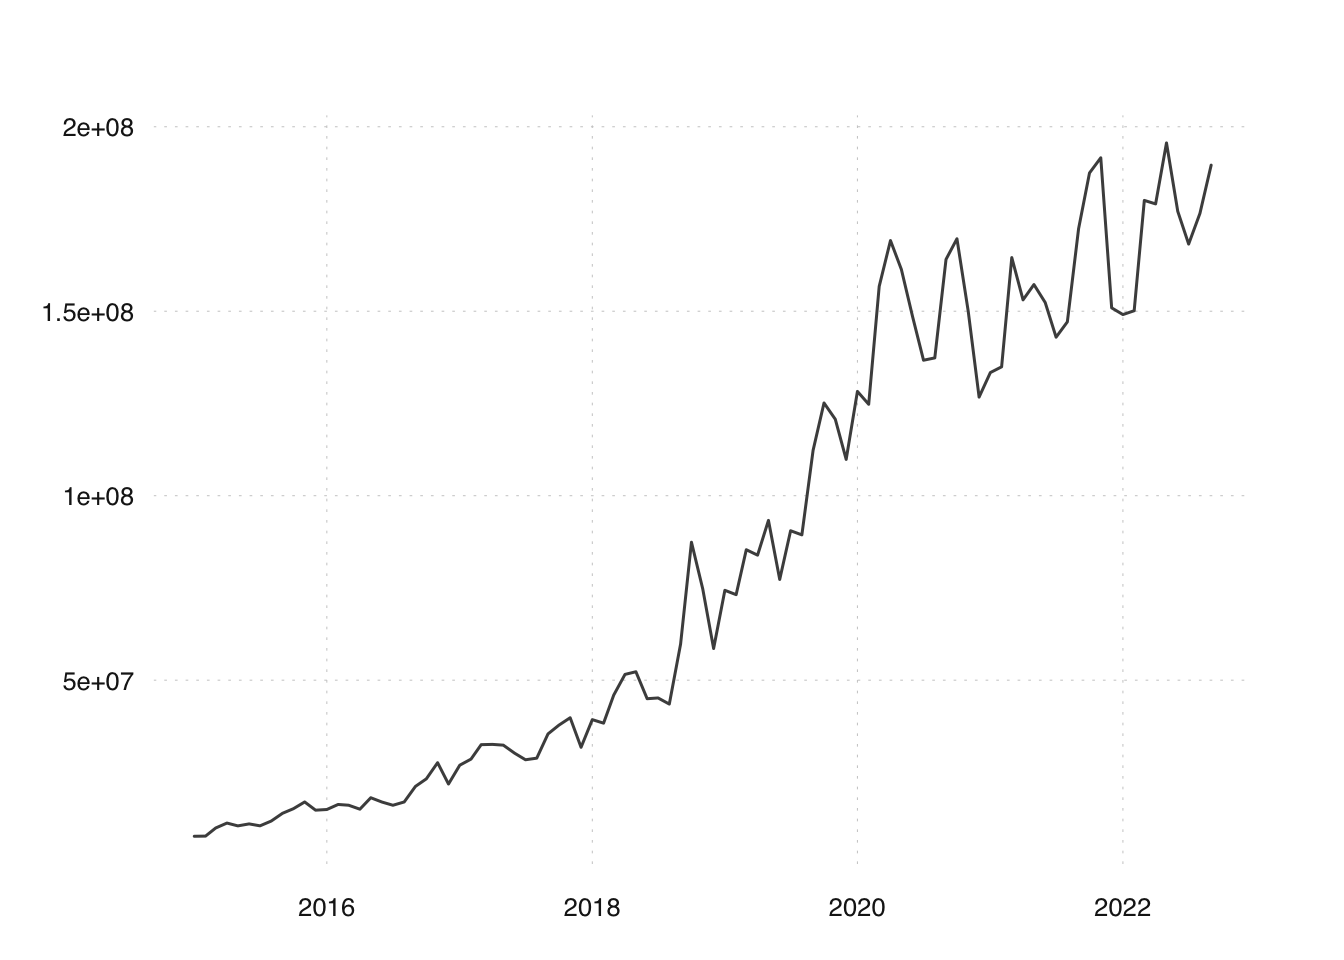
\includegraphics{./intro_files/figure-pdf/fig-cran-dl-1.pdf}

}

\caption{\label{fig-cran-dl}Monthly R Package Downloads. (Source:
RStudio CRAN mirror.)}

\end{figure}

\begin{Shaded}
\begin{Highlighting}[]
\FunctionTok{library}\NormalTok{(cranlogs)}
\FunctionTok{library}\NormalTok{(dplyr)}
\FunctionTok{library}\NormalTok{(lubridate)}
\FunctionTok{library}\NormalTok{(tsbox)}
\NormalTok{top }\OtherTok{\textless{}{-}}\NormalTok{ cranlogs}\SpecialCharTok{::}\FunctionTok{cran\_top\_downloads}\NormalTok{()}

\NormalTok{packs }\OtherTok{\textless{}{-}}\NormalTok{ cranlogs}\SpecialCharTok{::}\FunctionTok{cran\_downloads}\NormalTok{(}
                               \AttributeTok{from =} \StringTok{"2015{-}01{-}01"}\NormalTok{,}
                               \AttributeTok{to =} \StringTok{"2022{-}09{-}30"}\NormalTok{)}

\NormalTok{packs }\SpecialCharTok{|\textgreater{}} 
  \FunctionTok{group\_by}\NormalTok{(}\FunctionTok{floor\_date}\NormalTok{(date, }\StringTok{"month"}\NormalTok{)) }\SpecialCharTok{|\textgreater{}} 
  \FunctionTok{summarize}\NormalTok{(}\AttributeTok{m =} \FunctionTok{sum}\NormalTok{(count)) }\SpecialCharTok{|\textgreater{}} 
  \FunctionTok{ts\_plot}\NormalTok{()}
\end{Highlighting}
\end{Shaded}

Bandwagonism aside, source code can be a tremendously sharp, unambiguous
and international communication channel. Your web scraper does not work?
Instead of reaching out in a clumsy but wordy cry for help, posting what
you tried so far described by source code will often get you good
answers within hours. Platforms like
stack\index{stack}overflow\footnote{https://stack\index{stack}overflow.com}
or Crossvalidated\footnote{https://crossvalidated.com} do not only store
millions of questions and answers, they also gather a huge and active
community to discuss issues. Plus, recent developments show that source
code is not only useful to communicate with human experts. Have you
tried to turn an idea into code or improve a piece of code by playing
ping pong with chatGPT or Bing? Or think of feature requests: After a
little code ping pong with the package author, your wish eventually
becomes clearer. Let alone chats with colleagues and co-authors. Sharing
code just works. Academic journals have found that out, too. Many
outlets require you to make the data and source code behind your work
available. Social Science Data Editors (Vilhuber et al. 2022) is a
bleeding-edge project at the time of writing this, but it is already
referred to by top-notch journals like \emph{American Economic Review
(AER)}.

\begin{figure}

{\centering 
\includegraphics{./images/communication.png}

}

\caption{Source code is be unambiguous, interactive and global
communication channel. Source: own illustration.}

\end{figure}

In addition to the above reproducibility and ability to share, code
scales and automates. automation\index{automation} is very convenient;
like when you want to download data, process and create the same
visualization and put it on your website any given Sunday.
automation\index{automation} is inevitable; like when you have to gather
daily updates from different outlets or work through thousands of .pdfs.

Last but not least, programming enables you to do many things you
couldn't do without being an absolute guru (if at all) if it wasn't for
programming. Take visualization, for example. Go check the D3\index{D3}
Examples at https://d3js.org/. Now, try to do that in Excel. If you did
these things in Excel, it would make you an absolute spreadsheet
visualization Jedi, probably missing out on other time-consuming skills
to master. Yet, with decent, carpentry-level programming skills you can
already do so many spectacular things while not really specializing and
staying very flexible.

\hypertarget{why-work-like-an-operations-engineer}{%
\section{Why Work Like an Operations
Engineer?}\label{why-work-like-an-operations-engineer}}

While software \emph{development} has become closer to many researchers,
\emph{operations}, the second part of the term
\emph{DevOps\index{DevOps}}, is much further away from the average
researcher or business analyst. Why even think about operations? Because
we can afford to do so. Operations\index{DevOps} have become so much
more accessible in recent years, that many applications can be dealt
with single-handedly. Though one's production applications may still be
administered by operations professionals, the ability to create and run
a proof of concept from scratch is an invaluable skill. A running
example says more than a 15-page specification that fails to translate
business talk into tech talk. The other way around, something to look at
an early stage helps to acquire funds and convince managers and other
collaborators.

But people without a computer engineering background are by no means
limited to proof of concepts these days. Trends like cloud computing and
software-as-a-service products help developers focus on their expertise
and limit the amount of knowledge needed to host a service in secure and
highly available fashion.

Also, automation\index{automation} is key to the DevOps\index{DevOps}
approach and an important reason why DevOps\index{DevOps} thinking is
also very well suited for academic researchers and business analysts.
So-called \emph{continuous integration} can help to enforce a battery of
quality checks such as unit tests or installation checks. Let's say a
push to a certain branch of a git repository leads to the checks and
tests. In a typical workflow, successful completion of quality checks
triggers continuous deployment to a blog, rendering into a paper or
interactive data visualization.

By embracing both parts of the \emph{DevOps\index{DevOps}} approach,
researchers do not only gain extra efficiency, but more importantly they
improve reproducibility and therefore accountability and quality of
their work. The effect of a DevOps\index{DevOps} approach on quality
control is not limited to reproducible research in a publication sense
only, but also enforces rules during collaboration: no matter who
contributes, the contribution gets gut-checked and only deployed if
checks passed. Similar to the well established term \emph{software
carpentry} that advocates a solid, application minded understanding of
programming with data, I suggest a carpentry-level understanding of
development and operations is desirable for the programming data
analyst.

\hypertarget{how-to-read-this-book}{%
\section{How To Read This Book?}\label{how-to-read-this-book}}

The focal goal of this book is to map out the open source ecosystem,
identify neuralgic components and give you an idea of how to improve not
only in programming but also in navigating the wonderful but vast open
source world. Chapter 2 is the road map for this book: it describes and
classifies the different parts of the open source stack\index{stack} and
explains how these pieces relate to each other. Subsequent chapters
highlight core elements of the open source toolbox one at a time and
walk through applied examples, mostly written in the R language.

This book is the companion I wish I had when I started an empirical,
data intensive PhD in economics. Yet, the book is written years after my
PhD was completed and with the hindsight of more than 10 years in
academia. \emph{Research Software Engineering} is written based on the
experience of helping students and seasoned researchers of different
fields with their data management, processing and communication of
results.

If you are confident in your ambition to amp up your programming to at
least solid software carpentry\index{software carpentry}
level\footnote{https://software-carpentry.org/} within the next few
months, I suggest getting an idea of your starting point relative to
this book. The upcoming \emph{backlog} section is essentially a list of
suggested to-dos on your way to solid software carpentry. Obviously, you
may have cleared a few tasks of this backlog before reading this book
which is fine. On the other hand, you might not know about some of the
things that are listed in the \emph{requirement} section, which is fine,
too. The backlog and requirements section just mean to give you some
orientation.

If you do not feel committed, revisit the previous section, discuss the
need for programming with peers from your domain and possibly talk to a
seasoned R or Python\index{Python} programmer. Motivation and commitment
are key to the endurance needed to develop programming into a skill that
truly leverages your domain-specific expertise.

\hypertarget{backlog}{%
\section{Backlog}\label{backlog}}

If you can confidently say you can check all or most of the below, you
have reached \emph{carpentry} level in developing and running your
applications. Even if this level is your starting point, you might find
a few useful tips or simply may come to cherry-pick. In case you are
rather unfamiliar with most of the below, the contextualization, the
classification and overview of tools is likely the most valuable help
this book provides.

A solid, applied understanding of \textbf{git version control} and the
\textbf{collaboration workflow associated with git}\index{git} does not
only help you stay ahead of your own code; git proficiency makes you a
team player. If you are not familiar with commits, pulls, pushes,
branches, forks\index{fork} and pull requests, \emph{Research Software
Engineering} will open up a new world for you. An introduction to
industry standard collaboration makes you fit into a plethora of
(software) teams around the globe -- in academia and beyond.

Your backlog en route to a researcher who is comfortable in
\emph{Research Software Engineering} obviously contains a
\textbf{strategy to improve your programming} itself. To work with data
in the long run, an idea of the \textbf{challenges of data management}
from persistent storage to access restrictions should complement your
programming. Plus, modern data-driven science often has to handle
datasets so large, which is when
\textbf{infrastructure\index{infrastructure}} other than local desktops
come into play. Yet, high performance computing (HPC) is by far not the
only reason it is handy for a researcher to have a basic understanding
of \textbf{infrastructure\index{infrastructure}}. \textbf{Communication}
of results, including data dissemination or interactive online reports
require the content to be served from a server with permanent online
access. Basic workflow \textbf{automation\index{automation}} of regular
procedures, e.g., for a repeated extract-transform-load (ETL) process to
update data, is a low-hanging (and very useful) fruit for a programming
researcher.

The case studies at the end of the book are not exactly a backlog item
like the above but still a recommended read. The case studies in this
book are hands-on programming examples -- mostly written in R -- to
showcase tasks from application programming interface (API) usage to
geospatial visualization in reproducible fashion. Reading and actually
running other developers' code not only improve one's own code, but
helps to see what makes code inclusive and what hampers
comprehensibility.

\hypertarget{requirements}{%
\section{Requirements}\label{requirements}}

Even though \emph{Research Software Engineering} aims to be inclusive
and open to a broad audience with different starting points, several
prerequisites exist to get the most out of this book. I recommend you
have made your first experience with an interpreted programming language
like R or Python. Be aware though that experience from a stats or math
course does not automatically make you a programmer, as these courses
are rightfully focused on their own domain. Books like \emph{R for Data
Science} (Hadley Wickham and Grolemund 2017) or websites like the
\emph{The Carpentries}\footnote{https://carpentries.org/} help to
solidify your data science minded, applied programming. \emph{Advanced
R} (Hadley Wickham 2019), despite its daunting title, is an excellent
read to get past the superficial kind of understanding of R that we
might acquire from a first encounter in a stats course.

A certain familiarity with \emph{console/terminal basics} will help the
reader sail smoothly. At the end of the day, there are no real must-have
requirements to benefit from this book. The ability to self-reflect on
one's starting point remains the most important requirement to leverage
the book.

\emph{Research Software Engineering} willingly accepts to be
overwhelming at times. Given the variety of topics touched on in an
effort to show the big picture\{big picture\}, I encourage the reader to
remain relaxed about a few blanks even when it comes to fundamentals.
The open source community offers plenty of great resources to
selectively upgrade skills. This book intends to show how to evaluate
the need for help and how to find the right sources. If none of the
above means something to you, though, I recommend making yourself
comfortable with the basics of some of the above fields before you start
to read this book.

\bookmarksetup{startatroot}

\hypertarget{stack-a-developers-toolkit}{%
\chapter{\texorpdfstring{Stack\index{stack}: A Developer's
Toolkit}{Stack: A Developer's Toolkit}}\label{stack-a-developers-toolkit}}

The goal of this chapter (and probably the most important goal of this
entire book) is to help you see the big picture\index{big picture} of
which tool does what. The following sections will group common
programming-with-data components by purpose. All of the resulting groups
represent aspects of programming with data, and I will move on to
discuss these groups in a dedicated chapter each.

\begin{figure}

{\centering 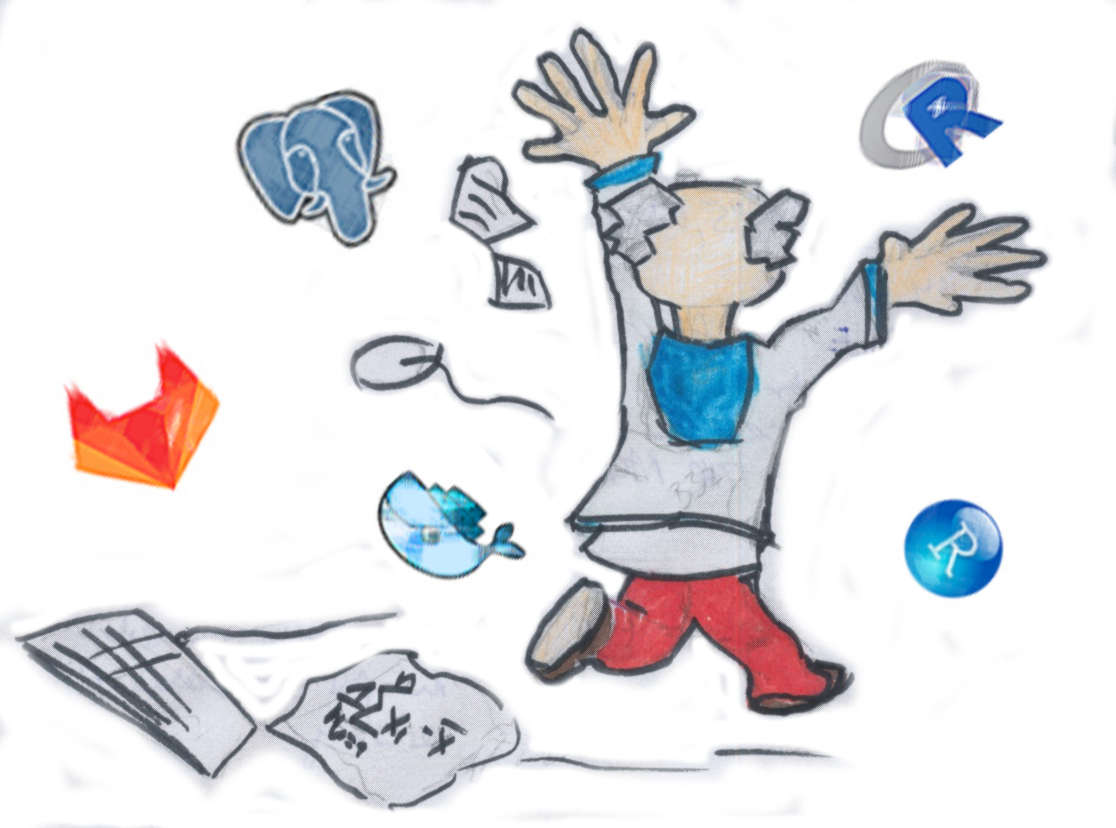
\includegraphics{./images/dr_egghead_panics.jpg}

}

\caption{Aaaaaaah! Don't panic, Dr.~Egghead! All these components are
here to help you and you won't need all of them from the start. (Source:
own illustration.)}

\end{figure}

Just like natural craftsmen, digital carpenters depend on their toolbox
and their mastery of it. A project's \emph{stack\index{stack}} is what
developers call the choice of tools used in a project. Even though
different flavors come down to personal preferences, there is a lot of
common ground in \emph{programming with data} stack\index{stack}s.
Table~\ref{tbl-stack} shows some of the components I use most often
grouped by their role. Of course, this is a personal choice. Obviously,
I do not use \emph{all} of these components in every single small
project. \emph{Git, R} and \emph{R Studio} would be a good minimal
version.\index{Woodpecker}

\hypertarget{tbl-stack}{}
\begin{table}
\caption{\label{tbl-stack}Components of Data Science Stack }\tabularnewline

\centering
\begin{tabular}{l>{\raggedright\arraybackslash}p{5.6cm}}
\toprule
Component & Choice\\
\midrule
Interpreter/Language & R, Python, JavaScript\\
IDE/Editor & R Studio, VS Code, Sublime\\
Version Control & Git\\
Project Management & GitHub, GitLab\\
database & PostgreSQL\\
\addlinespace
"Virtual" Environments & Docker\\
Communication (Visualization, Web) & Node, Quasar (vue.js)\\
Website Hosting & Netlify, GitHub Pages\\
Workflow automation & Apache Airflow\\
Continous Integration & Woodpecker, GitLab CI, GitHub Actions\\
\bottomrule
\end{tabular}
\end{table}

Throughout this book, often a choice for one piece of software needs to
be made to illustrate things. To get the most out of the book, keep in
mind that these choices are examples and try to focus on the role of an
item in the big picture\index{big picture}.

\hypertarget{programming-language}{%
\section{Programming Language}\label{programming-language}}

In Statistical Computing, the interface between the researcher and the
computation node is almost always an interpreted programming language as
opposed to a compiled one. Compiled languages like C++ require the
developer to write source code and compile, i.e., translate source code
into what a machine can work with \emph{before} runtime. The result of
the compilation process is a binary which is specific to an operating
system. Hence, you will need one version for Windows, one for OSX and
one for Linux if you intend to reach a truly broad audience with your
program. The main advantage of a compiled language is speed in terms of
computing performance, because the translation into machine language
does not happen during runtime. A reduction of development speed and
increase in required developer skills are the downside of using compiled
languages.

\begin{quote}
Big data is like teenage sex: everyone talks about it, nobody really
knows how to do it, everyone thinks everyone else is doing it, so
everyone claims they are doing it. -- Dan Ariely, Professor of
Psychology and Behavioral Economics on \emph{X}\footnote{https://x.com/danariely/status/287952257926971392}
\end{quote}

\newpage

The above quote became famous in the hacking data community, not only
because of the provocative, fun part of it, but also because of the
implicit advice behind it. Given the enormous gain in computing power in
recent decades, and also methodological advances, interpreted languages
are often fast enough for many social science problems. And even if it
turns out, your data grow out of your setup, a well-written proof of
concept written in an interpreted language can be a formidable
blueprint. \textbf{Source code is turning into an important scientific
communication channel.} Put your money on it, your interdisciplinary
collaborator from the High Performance Computing (HPC) group will prefer
some Python code as a briefing for their C++ or Fortran program over a
wordy description out of your field's ivory tower.

Interpreted languages are a bit like pocket calculators, you can look at
intermediate results, line-by-line. R and Python are the most popular
open source software (\protect\hyperlink{glossary}{OSS}) choices for
hacking with data, Julia (Bezanson et al. 2017) is an up-and-coming,
performance-focused language with a much slimmer ecosystem. A bit of
JavaScript can't hurt for advanced customization of graphics and online
communication of your results.

\hypertarget{interaction-environment}{%
\section{Interaction Environment}\label{interaction-environment}}

While the fact that a software developer needs to choose a programming
language to work with is rather obvious, the need to compose and
customize an environment to interact with the computer is much less
obvious to many. Understandably so because, outside of programming,
software such as word processors, video or image editors presents itself
to the user as a single program. That single program takes the user's
input, processes the input (in memory) and stores a result on disk for
persistence -- often in a proprietary, program specific format.

Yet, despite all the understanding for nonchalantly saying we keep
documents \textbf{in} Word or data \textbf{in} R Studio, it's beyond
nerdy nitpicking when I insist that data are kept in files (or
database\index{database}s) -- \textbf{not} in a program. And that R is
\textbf{not} R Studio: This sloppy terminology contributes to making us
implicitly accept that our office documents live in one single program.
(And that there is only one way to find and edit these files: through
said program).

It is important to understand that source code of essentially any
programming languages is a just a plain text file and therefore can be
edited in any editor. Editors come in all shades of gray: from lean,
minimal code highlighting support to full-fledged integrated development
environments (IDEs) with everything from version control integration to
sophisticated debugging.

Which way of interaction the developer likes better is partly a matter
of personal taste, but it also depends on the programming language, the
team's form of collaboration and size of the project. In addition to a
customized editor, most developers use some form of a console to
communicate with their operating system. The ability to send commands
instead of clicking is not only reproducible and shareable, but it also
outpaces mouse movement by a lot when commands come in batches.
Admittedly, configuration, practice and getting up to speed takes time,
but once you have properly customized the way you interact with your
computer when writing code, you will never look back.

In any case, make sure to customize your development environment: choose
the themes you like, make sure the cockpit you spent your day in is
configured properly and feels comfy.

\hypertarget{version-control}{%
\section{Version Control}\label{version-control}}

To buy into the importance of managing one's code professionally may be
the single most important take-away from this book. Being able to work
with \index{version control} will help you fit into numerous different
teams that have contact points with data science and programming, let
alone if you become part of a programming or data science team.

While \index{version control} has a long history dating back to
CVS\footnote{Concurrent Versions System: https://cvs.nongnu.org/} and
SVN\footnote{Apache Subversion}, the good news for the learner is, that
there is a single dominant approach when it comes to
\index{version control} in the data analysis world. Despite the fact
that its predecessors and alternatives such as Mercurial are still
around, git\footnote{https://git-scm.com/book/en/v2/Getting-Started-About-Version-Control}
is the one you have to learn. To learn more about the history of
\index{version control} and approaches other than git, Eric Sink's
\emph{Version Control by Example} (Sink 2011) is for you.

So what does git do for us as researchers? How is it different from
Dropbox?

\begin{verbatim}
git does not work like dropbox. git is not like dropbox.
git does not work like dropbox. git is not like dropbox. 
git does not work like dropbox. git is not like dropbox.
git does not work like dropbox. git is not like dropbox. 
git does not work like dropbox. git is not like dropbox.
git does not work like dropbox. git is not like dropbox. 
\end{verbatim}

The idea of thinking of a sync is what interferes with comprehension of
the benefit of \index{version control} (which is why I hate that git
\protect\hyperlink{glossary}{GUI}s call it ``sync'' anyway to avoid
irritation of user's initial beliefs.). Git is a decentralized
\index{version control} system that keeps track of a history of semantic
commits. Those commits may consist of changes to multiple files. A
commit message summarizes the gist of a contribution. \emph{Diffs} allow
comparing different versions.

\begin{figure}

{\centering 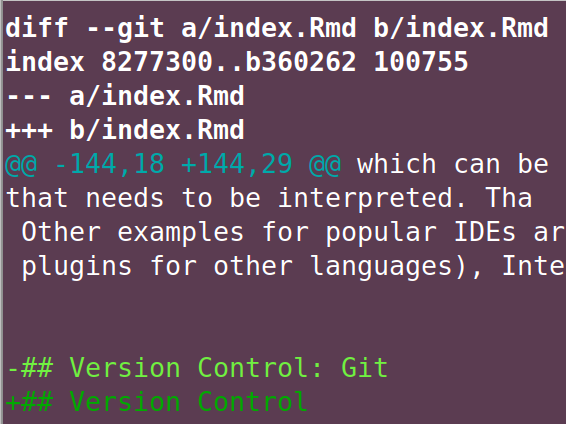
\includegraphics{./images/diff.png}

}

\caption{The \emph{diff} output shows an edit during the writing of this
book. The line preceded by `-' was replaced with the line preceded by
`+'.}

\end{figure}

Git is well suited for any kind of text file, whether it is source code
from Python or C++, or some text written in Markdown or LaTeX. Binaries
like .pdfs or Word documents are possible, too, but certainly not the
type of file for which git is really useful. This book contains a
detailed, applied introduction tailored to researchers in a dedicated
\index{version control} chapter, so let's dwell with the above
contextualization for a bit.

\hypertarget{data-management}{%
\section{Data Management}\label{data-management}}

One implication of bigger datasets and/or bigger teams is the need to
manage data. Particularly when projects establish themselves or update
their data regularly, well-defined processes, consistent storage and
possibly access management become relevant. But even if you worked
alone, it can be very helpful to have an idea about data storage in
files systems, memory consumption and archiving data for good.

Data come in various forms and dimensions, potentially deeply nested.
Yet, researchers and analysts are mostly trained to work with
one-row-one-observation formats, in which columns typically represent
different variables. In other words, two-dimensional representation of
data remains the most common and intuitive form of data to many. Hence,
office software offers different, text-based and proprietary spreadsheet
file formats. On disk, comma separated files (.csv)\footnote{Some
  dialects use different separators like `;' or tabs, partly because of
  regional differences like the use of commas as decimal delimiters.}
are probably the purest representation of two-dimensional data that can
be processed comfortably by any programming language and that can be
read by many programs. Other formats such as .xml or .json allow storing
even deeply nested data.

In-memory, that is when working interactively with programming languages
such as R or Python, data.frames are the most common representation of
two-dimensional data. Data.frames, their progressive relatives like
tibbles or data.tables and the ability to manipulate them in
reproducible, shareable and discussible fashion is the first superpower
upgrade over pushing spreadsheets. Plus, other representation such as
arrays, dictionaries or lists represent nested data in memory. Though
in-memory data manipulation is very appealing, memory is limited and
needs to be managed. Making the most of the memory available is one of
the driving forces behind extensions of the original data.frame concept.

The other obvious limitation of data in memory is the lack of persistent
storage. Therefore, in-memory data processing needs to be combined with
file based storage are a database\index{database}. The good news is that
languages like R and Python are well-equipped to interface with a
plethora of file-based approaches as well as database\index{database}s.
So well, that I often recommend these languages to researchers who work
with other less-equipped tools, solely as an intermediate layer.

To evaluate which relational (essentially SQL) or non-relational
database\index{database} to pick up just seems like the next daunting
task of stack\index{stack} choice. Luckily, in research, first
encounters with a database\index{database} are usually passive, in the
sense that you want to query data from a source. In other words, the
choice has been made for you. So unless you want to start your own data
collection from scratch, simply sit back, relax and let the internet
battle out another conceptual war. For now, let's just be aware of the
fact that a data management game plan should be part of any analysis
project.

\hypertarget{infrastructure}{%
\section{\texorpdfstring{infrastructure\index{infrastructure}}{infrastructure}}\label{infrastructure}}

For researchers and business analysts who want to program with data, the
starting infrastructure\index{infrastructure} is very likely their own
desktop or notebook computer. Nowadays, this already means access to
remarkable computing power suited for many tasks.

Yet, it is good to be aware of the many reasons that can turn the
infrastructure\index{infrastructure} choice from a no-brainer into a
question with many options and consequences. Computing power, repeated
or scheduled tasks, hard-to-configure or non-compatible runtime
environment, online publication or high availability may be some of the
needs that make you think about infrastructure\index{infrastructure}
beyond your own notebook.

Today, thanks to software-as-a-service (SaaS) offers and cloud
computing, none of the above needs imply running a server, let alone a
computing center on your own. Computing has not only become more
powerful over the last decade, but also more accessible. Entry hurdles
are lower than ever. Many needs are covered by services that do not
require serious upfront investment. It has become convenient to try and
let the infrastructure\index{infrastructure} grow with the project.

From a researcher's and analyst's perspective, one of the most
noteworthy infrastructure\index{infrastructure} developments of
recentness may be the arrival of \emph{containers} in data analysis.
Containers are isolated, single-purpose environments that run either on
a single container host or with an orchestrator in a cluster. Although
technically different from virtual machines, we can regard containers as
virtual computers running on a computer for now. With containers, data
analysts can create isolated, single purpose environments that allow to
reproduce analysis even after one's system was upgraded and with it all
the libraries used to run the analysis. Or think of some exotic LaTeX
configuration, Python environment or database\index{database} drivers
that you just can't manage to run on your local machine. Bet there is a
container blueprint (aka image) around online for exactly this purpose.

\begin{quote}
Premature optimization is the root of all evil. -- Donald Knuth.
\end{quote}

On the flip side, product offerings and therefore our options have
become a fast-growing, evolving digital jungle. So, rather than trying
to keep track (and eventually loosing it) of the very latest gadgets,
this book intends to show a big picture\{big picture\} overview and pass
on a strategy to evaluate the need to add to your
infrastructure\index{infrastructure}. Computing power, availability,
specific services and collaboration are the main drivers for researchers
to look beyond their own hardware. Plus, public exposure, i.e., running
a website as discussed in the publishing section, asks for a web host
beyond our local notebooks.

\hypertarget{automation}{%
\section{\texorpdfstring{Automation\index{automation}}{Automation}}\label{automation}}

``Make repetitive work fun again!'' could be the claim of this section.
Yet, it's not just the typical intern's or student assistant's job that
we would love to automate. Regular ingestion of data from an application
programming interface (API) or a web scraping process are one form of
reoccurring tasks, often called cron jobs after the Linux cron command,
which is used to schedule execution of Linux commands. Regular
computation of an index, triggered by incoming data would be a less
time-focused, but more event-triggered example of an automated task.

The one trending form of automation\index{automation}, though, is
\emph{continuous integration/continuous development
(CI/CD\index{CI/CD})}. \emph{CI/CD\index{CI/CD}} processes are typically
closely linked to a git \index{version control} repository and are
triggered by a particular action done to the repository. For example, in
case some pre-defined part (branch) of a git repository gets updated, an
event is triggered and some process starts to run on some machine
(usually some container). Builds of software packages are very common
use cases of such a \emph{CI/CD\index{CI/CD}} process. Imagine you are
developing an R package and want to run all the tests you've written,
create the documentation and test whether the package can be installed.
Once you've made your changes and push to your remote git repository,
your push triggers the tests, the check, the documentation rendering and
the installation. Potentially a push to the main branch of your
repository could even deploy a package that cleared all of the above to
your production server.

Rendering documentation, e.g., from Markdown to HTML\index{HTML} into a
website or presentation or a book like this one is a very similar
example of a CI/CD\index{CI/CD} process. Major git providers like Gitlab
(GitLab CI/CD\index{CI/CD}) or GiTHub (GitHub Actions) offer
CI/CD\index{CI/CD} tool integration. In addition, standalone services
like CircleCI can be used as well as open source, self-hosted software
like Woodpecker\index{Woodpecker} CI\footnote{https://woodpecker-ci.org/}.

\hypertarget{communication-tools}{%
\section{Communication Tools}\label{communication-tools}}

Its community is one of the reasons for the rise of open source software
over the last decades. Particularly, newcomers would miss a great chance
for a kick-start into programming if they did not connect with the
community. Admittedly, not all the community's communication habits are
for everyone, yet it is important to make your choices and pick up a few
channels.

Chat clients like Slack, Discord or the Internet Relay Chat (IRC) (for
the pre-millenials among readers) are the most direct form of
asynchronous communication. Though many of the modern alternatives are
not open source themselves, they offer free options and remain popular
in the community despite self-hosted approaches such as
matrix\footnote{https://matrix.org/} along with Element\footnote{https://element.io/}.
Many international groups around data science and statistical computing
such as RLadies or the Society of Research Software Engineering have
Slack spaces that are busy 24/7 around the world.

Social media is less directed and more easily consumed in a passive
fashion than a chat space. Over the last decade, \emph{X}, formerly
known as twitter, has been a very active and reliable resource for good
reads but has seen parts of the community switch to more independent
platforms such as Mastodon\footnote{https://mastodon.social/}. Linkedin
is another suitable option to connect and find input, particularly in
parts of the world where other platforms are less popular. Due to its
activity, social media is also a great way to stay up-to-date with the
latest developments.

Mailing lists are another, more old-fashioned form to discuss things.
They do not require a special client and just an e-mail address to
subscribe to their regular updates. If you intend to avoid social media,
as well as signing up at knowledge sharing platforms such as
stack\index{stack}overflow.com\footnote{https://stack\index{stack}overflow.com}
or reddit\footnote{https://reddit.com}, mailing lists are a good way to
get help from experienced developers.

Issue trackers are one form of communication that is often
underestimated by newcomers. Remotely hosted git repositories, e.g.,
repositories hosted at GitHub\index{GitHub} or GitLab, typically come
with an integrated issue trackers to report bugs. The community
discusses a lot more than problems on issue trackers: feature requests
are a common use case, and even the future direction of an open source
project may be affected substantially by discussions in its issue
tracker.

\hypertarget{publishing-and-reporting}{%
\section{\texorpdfstring{Publishing and
Reporting\index{reporting}}{Publishing and Reporting}}\label{publishing-and-reporting}}

Data analysis hopefully yields results that the analyst intends to
report internally within their organization or share with the broader
public. This has led to a plethora of options on the reporting end.
Actually, data visualization and reproducible, automated reporting are
two of the main drivers researchers and analysts turn to programming for
their data analysis.

In general, we can distinguish between two forms of output: pdf-like,
print-oriented output and HTML-centered web content. Recent tool chains
have enabled analysts without strong backgrounds in web frontend
development (HTML/CSS/JavaScript) to create nifty reports and
impressive, interactive visualizations. Frameworks like R Shiny or
Python Dash even allow creating complex interactive websites.

Notebooks that came out of the Python world established themselves in
many other languages implementing the idea of combining text with code
chunks that get executed when the text is rendered to HTML\index{HTML}
or PDF. This allows researchers to describe, annotate and discuss
results while sharing the code that produced the results described. In
academia, progressive scholars and journals embrace this form of
creating manuscripts as \emph{reproducible research} that improves trust
in the presented findings.

Besides academic journals that started to require researchers to hand in
their results in reproducible fashion, reporting based on so-called
static website generators\footnote{As opposed to content management
  systems (CMS) that keep content in a database\index{database} and put
  content and layout template together when users visit a website,
  static website generators render a website once triggered by an event.
  If users want to update a static website, they simply rerun the render
  process and push the HTML output of said process online.} has taken
data blogs and reporting outlets including presentations by storm.
Platforms like GitHub render Markdown files to HTML automatically,
displaying formatted plain text as a decent website. Services such as
Netlify allow using a broad variety of build tools to render input that
contains text and code.

Centered around web browsers to display the output, HTML\index{HTML}
reporting\index{reporting} allows creating simple reports, blogs, entire
books (like this one) or presentation slides for talks. But thanks to
document converters like Pandoc and a typesetting juggernaut called
LaTeX, rendering sophisticated .pdf is possible, too. Some environments
even allow rendering to proprietary word processor formats.

\bookmarksetup{startatroot}

\hypertarget{programming-101}{%
\chapter{Programming 101}\label{programming-101}}

Obviously, the craft of \emph{programming} is essential to handling data
with a programming language. Though programming languages can differ
quite a bit from each other, there is common ground and an approach to
programming that is crucial to understand and important to learn by --
particularly for programmers without a formal computer science
background. This chapter points researchers, analysts and data
scientists to the low-hanging, high-impact fruits of software
engineering.

\emph{Programming is a form of communication}, a form of communication
with others and also with your future self. It actually may be the best
way to define complex contexts in reproducible fashion. Therefore,
source code needs to be written in inclusive fashion. Programming needs
to be seen as a chance to make complexity accessible to those who are
not experts in a particular domain. The fact that programs actually run
makes them more accessible to many than formal mathematical definitions.

The programming examples in this book mostly stick to the \emph{R}
language, which is easy to install and run on one's own local computer.
All the concepts shown easily transfer to other languages. Though
potentially a bit more tricky to install and run across operating
systems, Python\index{Python} would have been an equally good choice.
There had to be a decision for one language for this book.

\hypertarget{the-choice-that-doesnt-matter}{%
\section{The Choice That Doesn't
Matter}\label{the-choice-that-doesnt-matter}}

The very first (and intimidating) choice a novice hacker faces is which
is the programming language to learn. Unfortunately, the medium
popularly summed up as the internet offers a lot of really, fantastic
advice on the matter. The problem is, however, that this advice does not
necessarily agree which language is the best for research. In the realm
of data science -- get accustomed to that label if you are a scientist
who works with data -- the debate basically comes down to two languages:
The R Language for Statistical Computing and Python.

At least to me, there is only one valid advice: \textbf{It simply does
not matter}. If you stick around in data science long enough, you will
eventually get in touch with both languages and, in turn, learn both.
There is a huge overlap of what you can do with either of those
languages. R came out of the rather specific domain of statistics more
than 25 years ago and made its way to a more general programming
language thanks to over 20K extension packages (and counting). Built by
a mathematician, Python\index{Python} continues to be as general purpose
as it has ever been. But it got more scientific, thanks to extension
packages of its own such as pandas\footnote{https://pandas.pydata.org/},
SciPy\footnote{https://www.scipy.org/} or NumPy\footnote{https://numpy.org/}.
As a result, there is a huge overlap of what both languages can do, and
both will extend your horizon in unprecedented fashion if you did not
use a full-fledged programming language for your analysis beforehand.

\begin{figure}

{\centering 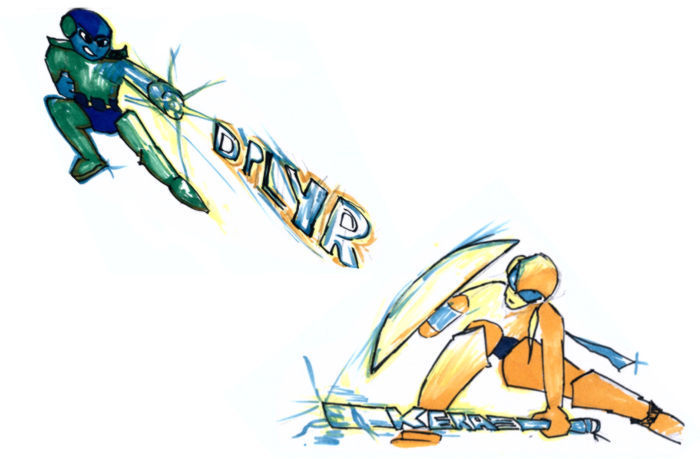
\includegraphics{./images/languagewar.jpg}

}

\caption{R: ``Dplyr smokes pandas.'' Python: ``But Keras is better for
ML!'' Language wars can be entertaining, sometimes spectacular, but most
of the time they are just useless. (Source: own illustration).}

\end{figure}

But why is there such a heartfelt debate online if it doesn't matter?
Let's pick up a random argument from this debate: R is easier to set up
and Python is better for machine learning. If you worked with Java or
another environment that's rather tricky to get going, you are hardened
and might not cherish easy onboarding. If you got frustrated before you
really started, you might feel otherwise. You may just have been unlucky
making guesses about a not so well-documented paragraph, trying to
reproduce a nifty machine learning blog post. Or imagine the frustration
in case just had installed the wrong version of Python or did not manage
to make sense of \emph{virtualenv} right from the beginning.

The point is, rest assured, if you just start doing analytics using a
programming language, both languages are guaranteed to carry you a long
way. There is no way to tell for sure which one will be the more
dominant language 10 years from now, or whether both will be around
holding their ground the way they do now. But once you reached a decent
software carpentry level in either language, it will help you a lot
learning the other. If your peers work with R, start with R; if your
close community works with Python, start with Python. If you are in for
the longer run, either language will help you understand the concepts
and ideas of programming with data. Trust me, there will be a natural
opportunity to get to know the other.

If you associate programming more often than not with hours of fiddling,
tweaking and fighting to galvanize approaches found online, this chapter
is for you. Don't expect lots of syntax. If you came for examples of
useful little programs from data visualization to parallel computing,
check out the \protect\hyperlink{case-studies}{Case Studies}.

The following sections share a blueprint to go from explorative script
to production-ready package. Organize your code and accompany the
evolution of your project: start out with experiments, define your
interface, narrow down to a proof of concept and scale up. Hopefully,
the tips, tricks and the guidance in this chapter will help you to
experience the rewarding feeling of a software project coming together
like a plan originated by Hannibal Smith\footnote{Google me!}.

\hypertarget{plan-your-program}{%
\section{Plan Your Program}\label{plan-your-program}}

How much planning ahead is optimal for your project ultimately depends
on your experience, number of collaborators and the size of your
project. But still, a rough standard checklist helps any project.

\hypertarget{think-library}{%
\subsection{Think Library!}\label{think-library}}

\begin{figure}

{\centering 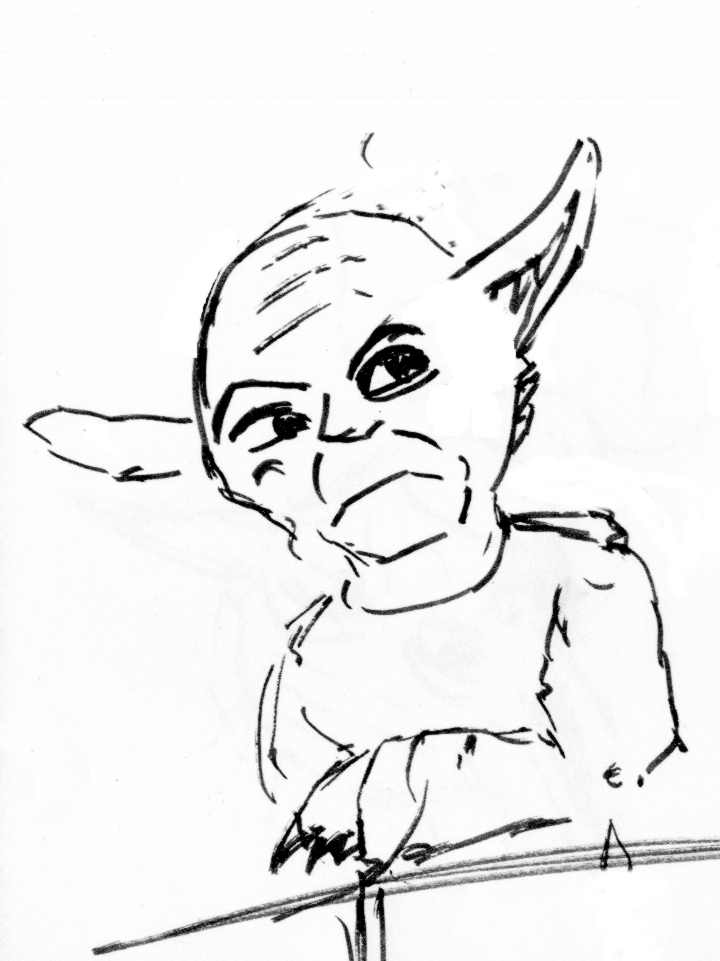
\includegraphics{./images/packages.jpg}

}

\caption{``Over the days are when creating packages for gurus was
only.'' (Source: own illustration.)}

\end{figure}

The approach that I find practical for applied, empirical research
projects involving code is: think library. Think package. Think
\emph{reusable} code. Don't think you can't do it. Let me demystify
packages for you: \textbf{Packages are nothing but source code organized
in folders following some convention}. Thanks to modern IDEs, it has
never been easier to stay inline with conventions. Editors like RStudio
ship with built-in support to create package skeletons with a few
clicks. Thousands of open source extension packages allow you to learn
from their structure. Tutorials like Packaging Python
Projects\footnote{https://packaging.python.org/tutorials/packaging-projects/}
or Hadley Wickham's book *R Packages (H. Wickham 2015) explain how to
create packages good enough to make the official PyPi or CRAN package
repositories.

In other words, it is unlikely that someone with moderate experience
comes with the best folder structure ever invented. Sure, every project
is different and not every aspect (folder) is needed in every project.
Nevertheless, there are well-established blueprints, guides and
conventions that suit almost any project. Unlike Office type of projects
which center around one single file, understand that a research project
will live in a folder with many subfolders and files. Not in one single
file.

Trust me on this one: The package approach will pay off early. Long
before you ever thought about publishing your package. Write your own
function definition, rather than just calling functions line-by-line.
Write code as if you need to make sure it runs on another computer.
Write code as if you need to maintain it.

Go from scripts like this\index{reproducible example}

\begin{Shaded}
\begin{Highlighting}[]
\CommentTok{\# This is just data for the sake of }
\CommentTok{\# reproducible example}
\FunctionTok{set.seed}\NormalTok{(}\DecValTok{123}\NormalTok{)}
\NormalTok{d1 }\OtherTok{\textless{}{-}} \FunctionTok{rnorm}\NormalTok{(}\DecValTok{1000}\NormalTok{)}
\NormalTok{d2 }\OtherTok{\textless{}{-}} \FunctionTok{rnorm}\NormalTok{(}\DecValTok{1000}\NormalTok{)}

\CommentTok{\# let\textquotesingle{}s create some custom descriptive}
\CommentTok{\# stats summary for the data generated above}
\NormalTok{d1\_mean }\OtherTok{\textless{}{-}} \FunctionTok{mean}\NormalTok{(d1)}
\NormalTok{d1\_sd }\OtherTok{\textless{}{-}} \FunctionTok{sd}\NormalTok{(d1)}
\NormalTok{d1\_q }\OtherTok{\textless{}{-}} \FunctionTok{quantile}\NormalTok{(d1)}
\NormalTok{desc\_stats\_d1 }\OtherTok{\textless{}{-}} \FunctionTok{list}\NormalTok{(}\AttributeTok{d1\_mean =}\NormalTok{ d1\_mean,}
                      \AttributeTok{d1\_sd =}\NormalTok{ d1\_sd,}
                      \AttributeTok{d1\_q =}\NormalTok{ d1\_q)}

\NormalTok{d2\_mean }\OtherTok{\textless{}{-}} \FunctionTok{mean}\NormalTok{(d2)}
\NormalTok{d2\_sd }\OtherTok{\textless{}{-}} \FunctionTok{sd}\NormalTok{(d2)}
\NormalTok{d2\_q }\OtherTok{\textless{}{-}} \FunctionTok{quantile}\NormalTok{(d2)}
\NormalTok{desc\_stats\_d2 }\OtherTok{\textless{}{-}} \FunctionTok{list}\NormalTok{(}\AttributeTok{d2\_mean =}\NormalTok{ d2\_mean,}
                      \AttributeTok{d2\_sd =}\NormalTok{ d2\_sd,}
                      \AttributeTok{d2\_q =}\NormalTok{ d2\_q)}
\end{Highlighting}
\end{Shaded}

To function definitions and calls like that

\begin{Shaded}
\begin{Highlighting}[]
\CommentTok{\# Imagine you had thousand of datasets.}
\CommentTok{\# Imagine you wanted to add some other stats}
\CommentTok{\# Imagine all the error prone c\&p with }
\CommentTok{\# the above solution. }
\CommentTok{\# Think of how much easier this is to document. }
\CommentTok{\# This is automation\textbackslash{}index\{automation\}. Not cooking. }
\NormalTok{create\_basic\_desc }\OtherTok{\textless{}{-}} \ControlFlowTok{function}\NormalTok{(distr)\{}
\NormalTok{  out }\OtherTok{\textless{}{-}} \FunctionTok{list}\NormalTok{(}
    \AttributeTok{mean =} \FunctionTok{mean}\NormalTok{(distr),}
    \AttributeTok{sd =} \FunctionTok{sd}\NormalTok{(distr),}
    \AttributeTok{quantiles =} \FunctionTok{quantile}\NormalTok{(distr)}
\NormalTok{  )}
\NormalTok{  out}
\NormalTok{\}}
\end{Highlighting}
\end{Shaded}

\begin{Shaded}
\begin{Highlighting}[]
\FunctionTok{create\_basic\_desc}\NormalTok{(d1)}
\end{Highlighting}
\end{Shaded}

\begin{verbatim}
$mean
[1] 0.01612787

$sd
[1] 0.991695

$quantiles
          0%          25%          50%          75%         100% 
-2.809774679 -0.628324243  0.009209639  0.664601867  3.241039935 
\end{verbatim}

\begin{Shaded}
\begin{Highlighting}[]
\FunctionTok{create\_basic\_desc}\NormalTok{(d2)}
\end{Highlighting}
\end{Shaded}

\begin{verbatim}
$mean
[1] 0.04246525

$sd
[1] 1.009674

$quantiles
         0%         25%         50%         75%        100% 
-3.04786089 -0.65322296  0.05485238  0.75345037  3.39037082 
\end{verbatim}

Start to document functions and their parameters using Roxygen (Hadley
Wickham et al. 2022) syntax, and you're already very close to creating
your first package.

\begin{tcolorbox}[enhanced jigsaw, left=2mm, arc=.35mm, colbacktitle=quarto-callout-tip-color!10!white, breakable, colframe=quarto-callout-tip-color-frame, bottomrule=.15mm, bottomtitle=1mm, colback=white, leftrule=.75mm, coltitle=black, toptitle=1mm, titlerule=0mm, title=\textcolor{quarto-callout-tip-color}{\faLightbulb}\hspace{0.5em}{Tip}, opacityback=0, rightrule=.15mm, toprule=.15mm, opacitybacktitle=0.6]

Hit Cmd+Alt+Shift+R\footnote{On Windows/Linux use Ctrl instead of Cmd.}
while inside a function definition with your cursor. When working with R
Studio, it will create a nifty Roxygen skeleton with all your function's
parameters.

\end{tcolorbox}

\begin{Shaded}
\begin{Highlighting}[]
\CommentTok{\#\textquotesingle{} Create Basic Descriptive Statistics}
\CommentTok{\#\textquotesingle{}}
\CommentTok{\#\textquotesingle{} Creates means, standard deviations and default}
\CommentTok{\#\textquotesingle{} quantiles from an numeric input vector. }
\CommentTok{\#\textquotesingle{} }
\CommentTok{\#\textquotesingle{} @param distr numeric vector drawn from an}
\CommentTok{\#\textquotesingle{} arbitraty distribution. }
\CommentTok{\#\textquotesingle{} @export }
\NormalTok{create\_basic\_desc }\OtherTok{\textless{}{-}} \ControlFlowTok{function}\NormalTok{(distr)\{}
\NormalTok{  out }\OtherTok{\textless{}{-}} \FunctionTok{list}\NormalTok{(}
    \AttributeTok{mean =} \FunctionTok{mean}\NormalTok{(distr),}
    \AttributeTok{sd =} \FunctionTok{sd}\NormalTok{(distr),}
    \AttributeTok{quantiles =} \FunctionTok{quantile}\NormalTok{(distr)}
\NormalTok{  )}
\NormalTok{  out}
\NormalTok{\}}
\end{Highlighting}
\end{Shaded}

Writing \emph{reusable code} will improve your ability to remember
syntax and apply concepts to other problems. The more you do it, the
easier and more natural it becomes. Just like a toddler figuring out how
to speak in a natural language. At first, progress seems small, but once
kids understand the bits and pieces of a language, they start building
at a remarkable speed, learn and never forget again.

\hypertarget{documentation}{%
\subsection{Documentation}\label{documentation}}

First things first. Write the first bit of documentation before your
first line of code. Documentation \textbf{written} with hindsight will
always be written with an all-knowing, smartest-person-in-the-room
mindset and the motivation of someone who already gave their best
programming. Understand, I am not talking about the fine-tuning here,
but about a written outline. Describe \textbf{how} parts of the code are
going to do stuff. Also, examples can't hurt to illustrate what you
meant. Research projects often take breaks, and getting back to work
after months should be as easy as possible.

\emph{Pseudocode} is a good way of writing up such an outline
documentation. Take a simple application programming interface (API)
wrapper, for example. Assume there is an API that returns numeric IDs of
hit entries when queried for keywords. These IDs can be passed on to yet
another \protect\hyperlink{glossary--}{endpoint}, to obtain a profile. A
rough game plan for an API Wrapper could look like this:

\begin{Shaded}
\begin{Highlighting}[]

\CommentTok{\# function: }
\CommentTok{\# keyword\_search(}
\CommentTok{\#  keyword,}
\CommentTok{\#  url = "https://some.default.url.com"}
\CommentTok{\#)}
\CommentTok{\# returns numeric ids according to some}
\CommentTok{\# api documentation}

\CommentTok{\# function: query\_profile(vec\_in\_ids)}
\CommentTok{\# a json object that should be immediately}
\CommentTok{\# turned into list by the function, }
\CommentTok{\# returns list of properties}
\end{Highlighting}
\end{Shaded}

Documentation should use your ecosystem's favorite documentation
framework. Yet, your comments within the code are the raw, initial form
of documentation. Comments help to understand key parts of a program as
well as caveats. Comments help tremendously during development time,
when debugging or coming back to a project. Let alone when joining a
project started by others.

While pseudocode where comments mimmick code itself is the exception to
that rule, good comments should always follow the
\textbf{not-what-but-why} principle. Usually, most high-level
programming languages are fairly easy to read and remind of rudimentary
English. Therefore, a \emph{what} comment like this is considered rather
useless:

\begin{Shaded}
\begin{Highlighting}[]
\CommentTok{\# compute the cumulative sum of a vector}
\FunctionTok{cumsum}\NormalTok{(}\FunctionTok{c}\NormalTok{(T,F,F,F,F,T,F,F,T,F,F,F,T))}
\end{Highlighting}
\end{Shaded}

Whereas this \emph{why} comment may actually be helpful:

\begin{Shaded}
\begin{Highlighting}[]
\CommentTok{\# use the fact that TRUE is actually stored as 1 }
\CommentTok{\# to create a sequence until the next true}
\CommentTok{\# this is useful for splitting the data later on.}
\FunctionTok{cumsum}\NormalTok{(}\FunctionTok{c}\NormalTok{(T,F,F,F,F,T,F,F,T,F,F,F,T))}
\end{Highlighting}
\end{Shaded}

Comment on why you do things, especially with which plan for future use
in mind. Doing so will certainly foster exchange with others who enter
or re-visit the code at a later stage (including yourself).

\hypertarget{design-your-interface}{%
\subsection{Design Your Interface}\label{design-your-interface}}

In many languages, it is fairly common to define the data type of both:
the input and the output\footnote{See statically typed language
  vs.~dynamically typed language.}. Though doing so is not necessary in
R, it is good practice to define the types of all parameters and results
in your comments/documentation.

Once you know a bit more about your direction of travel, it's time to
think about how to modularize your program. How do different parts of
the program play together? How do users interact with your program? Will
your code just act as a storage pit of tools, a loose collection of
commands for ad hoc use? Are others using the program, too? Will there
be machine-to-machine interaction? Do you need a graphical user
interface (GUI) like a Shiny app?

These questions will determine whether you use a strictly functional
approach\footnote{http://adv-r.had.co.nz/Functional-programming.html}, a
rudimentary form of object orientation like S3\footnote{http://adv-r.had.co.nz/OO-essentials.html}
(Hadley Wickham 2019), a stricter implementation like {[}R6 (Chang 2021)
or something completely exotic. There are plenty of great resources out
there, so I will not elaborate on this for the moment. The main message
of this section is: Think about the main use case. Is it interactive? Is
it a program that runs in batch, typically? Do your users code? Would
they prefer a GUI?

\hypertarget{dependencies}{%
\subsection{Dependencies}\label{dependencies}}

One important word of advice for novice package developers is to think
about your dependencies. Do not take dependencies lightly. Of course, it
is intriguing to stand on the shoulders of giants. Isn't R great because
of its over 20K extension packages? Isn't exactly this was made R such
as popular language?

Yes, extension packages are cool. Yes, the ease with which CRAN packages
are distributed is cool. But, just because packages are easy to install
and free of license costs, it does not mean leaning on plenty of
packages comes at no costs: One needs to stay informed about updates,
issues, breaking changes or undesired interdependencies between
packages.

The problem is mitigated a bit when (a) package is required in an
interactive script and (b) one is working with a very popular package.
Well-managed packages with a lot of
\protect\hyperlink{glossary--}{reverse dependencies} tend to deprecate
old functionality more smoothly, as authors are aware of the issues
breaking changes cause to a package's ecosystem.

In R, the \emph{tidyverse} bundle of packages seems ubiquitous and easy
to use, but it leads to quite a few dependencies. The data.table
ecosystem might be less popular but provides its functionality with a
single R package dependency (the \{methods\} package).

Often it does not take much to get rid of dependency:

\begin{Shaded}
\begin{Highlighting}[]
\FunctionTok{library}\NormalTok{(stringr)}
\NormalTok{cow }\OtherTok{\textless{}{-}} \StringTok{"A cow sounds off: mooooo"}
\FunctionTok{str\_extract}\NormalTok{(cow,}\StringTok{"moo+"}\NormalTok{)}
\end{Highlighting}
\end{Shaded}

\begin{verbatim}
[1] "mooooo"
\end{verbatim}

Sure, the above code is more intuitive, but shrewd use of good ol'
\emph{gsub} and back-referencing allows you to do the very same thing in
base R.

\begin{Shaded}
\begin{Highlighting}[]
\FunctionTok{gsub}\NormalTok{(}\StringTok{"(.+)(mooo+)"}\NormalTok{,}\StringTok{"}\SpecialCharTok{\textbackslash{}\textbackslash{}}\StringTok{2"}\NormalTok{,cow)}
\end{Highlighting}
\end{Shaded}

\begin{verbatim}
[1] "mooooo"
\end{verbatim}

Again, \{stringr\} (Hadley Wickham 2022b) is certainly a well-crafted
package, and it is definitely not the worst of all packages. But when
you just loaded a package because it adds convenience to one single line
or worse just because you found your solution online, think again before
adding more dependencies to a production environment.

\hypertarget{folder-structure}{%
\subsection{Folder Structure}\label{folder-structure}}

In R, packages may have the following folders. Note that this does not
mean a package has to contain all of these folders. FWIW, an R package,
needs to have NAMESPACE and DESCRIPTION files, but that is not the point
here. Also, there are more comprehensive, better books on the matter
than this little section. The point of this section though is to discuss
the role of folders and how they help you structure your work, even if
you don't want to create an R package in the first place.

This chapter describes the role of different folders in a package and
what these folders are good for. More likely than not, this will cover a
lot of the aspects of your project, too.

\begin{itemize}
\tightlist
\item
  R
\item
  data
\item
  docs
\item
  vignettes
\item
  src
\item
  inst
\item
  man
\end{itemize}

The below description explains the role of all of these folders.

\textbf{R}

The \emph{R} folder stores function definitions as opposed to function
calls. Typically every function goes into a separate file. Sometimes, it
makes sense to group multiple functions into a single file when
functions are closely related. Another reason for putting more than one
function into a single file is when you have a collection of relatively
simple, short helper functions. The R folder MUST NOT contain
calls\footnote{Essentially, examples are calls, too. Note, I do
  recommend adding examples. Hadley Wickham's guide to documenting
  functions within packages (H. Wickham 2015) shows how to add examples
  correctly.}.

\begin{Shaded}
\begin{Highlighting}[]
\NormalTok{my\_func\_def }\OtherTok{\textless{}{-}} \ControlFlowTok{function}\NormalTok{(param1, param2)\{}
  \CommentTok{\# here goes the function body, i.e.,}
  \CommentTok{\# what the function does}
\NormalTok{  a }\OtherTok{\textless{}{-}}\NormalTok{ (param1 }\SpecialCharTok{+}\NormalTok{ param2) }\SpecialCharTok{*}\NormalTok{ param3}
  \CommentTok{\# Note that in R, return statements are}
  \CommentTok{\# not necessary and even}
  \CommentTok{\# relatively uncommon, R will return}
  \CommentTok{\# the last unassigned statement}
  \FunctionTok{return}\NormalTok{(a)}
\NormalTok{\}}
\end{Highlighting}
\end{Shaded}

\textbf{man}

This folder contains the context manual of your package. What you'll
find here is the so-called \emph{function reference}, basically a
function and dataset-specific documentation. It's what you see when you
run \texttt{?function\_name}. The content of the \texttt{man/} folder is
usually created automatically from the \emph{Roxygen} style
documentation (note the \#' styled comments) during a
`\texttt{devtools::document()} run. Back in the days when people wore
pijamas and lived life slow, the man folder was filled up manually with
some LaTeX reminiscent .rd files, but ever since R Studio took over in
2012, most developers use \emph{Roxygen} and render the function
reference part of the documentation from their comments.

\begin{Shaded}
\begin{Highlighting}[]
\CommentTok{\#\textquotesingle{} Sum of Parameters Multiplied by First Input}
\CommentTok{\#\textquotesingle{}}
\CommentTok{\#\textquotesingle{} This functions only exists as a show case. }
\CommentTok{\#\textquotesingle{} It\textquotesingle{}s useless but nevertheless exported}
\CommentTok{\#\textquotesingle{} to the NAMESPACE of this}
\CommentTok{\#\textquotesingle{} package so users can see it and}
\CommentTok{\#\textquotesingle{}  call the function by it\textquotesingle{}s name.}
\CommentTok{\#\textquotesingle{}}
\CommentTok{\#\textquotesingle{} @param param1 numeric input }
\CommentTok{\#\textquotesingle{} @param param2 numeric input }
\CommentTok{\#\textquotesingle{} @export}
\NormalTok{my\_func\_def }\OtherTok{\textless{}{-}} \ControlFlowTok{function}\NormalTok{(param1, param2)\{}
  \CommentTok{\# here goes the function body, i.e.,}
  \CommentTok{\# what the function does}
\NormalTok{  a }\OtherTok{\textless{}{-}}\NormalTok{ (param1 }\SpecialCharTok{+}\NormalTok{ param2) }\SpecialCharTok{*}\NormalTok{ param1}
  \CommentTok{\# Note that in R, return statements are}
  \CommentTok{\# not necessary and even}
  \CommentTok{\# relatively uncommon, R will return}
  \CommentTok{\# the last unassigned statement}
  \FunctionTok{return}\NormalTok{(a)}
\NormalTok{\}}
\end{Highlighting}
\end{Shaded}

\textbf{docs}

This folder is typically not filled with content manually. When pushed
to GitHub\index{GitHub} a docs folder can easily be published as website
using Github Pages\footnote{https://pages.github.com/}. With GitHub
Pages you can host a decently styled modern website for free. Software
projects often use GitHub Pages to market a product or project or simply
for documentation purposes. All you need to do is check a couple of
options inside the Github Web GUI and make sure the docs/ folder
contains .md or .html files as well as stylesheets (.css). The latter
may sound a bit like Latin to people without a basic web development
background, but there is plenty of help. The R ecosystem offers
different flavors of the same idea: use a bit of markdown + R to
generate website code. There is the \{blogdown\} R package (Xie, Hill,
and Thomas 2017) for your personal website or blog. There is \{pkgdown\}
(Hadley Wickham, Hesselberth, and Salmon 2022) for your packages
documentation. And there is even bookdown to write an online book like
this. Write the Markdown file, render it as HTML\index{HTML} into the
docs folder and push the docs folder to GitHub. Done. Your website will
be online at username.github.io/reponame.

Here is a an example of a \{pkgdown\} website:

https://mbannert.github.io/timeseriesdb/

\textbf{data}

If you have file-based data like .csv, .RData, .json or even .xlsx, put
them in here. Keeping data in a separate folder inside the project
directory helps to keep reference to the data relative. There is nothing
more novice than
\texttt{read.csv("C:\textbackslash{}mbannert\textbackslash{}My\ Documents\textbackslash{}some\_data.csv")}.
Even if you like this book, I doubt you have a folder named `mbannert'
on your computer. Ah, and in case you wondered, extensive use of
\texttt{setwd()} is even worse. Keep your reference to data (and
functions alike) relative. If you are sourcing data from a remote NAS
drive as it is common at many universities, you can simply mount this
drive to your folder (LTMGTFY: How to mount a network drive
Windows/OSX).

\begin{tcolorbox}[enhanced jigsaw, left=2mm, arc=.35mm, colbacktitle=quarto-callout-note-color!10!white, breakable, colframe=quarto-callout-note-color-frame, bottomrule=.15mm, bottomtitle=1mm, colback=white, leftrule=.75mm, coltitle=black, toptitle=1mm, titlerule=0mm, title=\textcolor{quarto-callout-note-color}{\faInfo}\hspace{0.5em}{Note}, opacityback=0, rightrule=.15mm, toprule=.15mm, opacitybacktitle=0.6]

To actually bundle data into packages, I recommend to use a
\texttt{data-raw} folder for data formats other than native R formats.
From the raw folder, go on to process these raw files into R
representations that are then stored in \texttt{data}. The \{usethis\} R
package (Hadley Wickham et al. 2023) is a modern boilerplate approach
and suggest a smooth packaging workflow.

\end{tcolorbox}

\textbf{vignettes}

Admittedly not the most intuitive names for a folder that is supposed to
contain articles. Vignettes are part of the documentation of a good
package. It's kind of a description as if you were to write a paper
about your package, including some examples of how to use it. For modern
packages, vignettes are often part of their package down based online
documentation. Feel free, to name this folder differently, though
sticking to the convention will make it easier to turn your project into
a project at a later stage. This folder typically contains Markdown or
RMarkdown files.

\textbf{src}

The source folder is just here for the sake of completeness and is not
needed in projects that only involve R source code. It's reserved for
those parts of a package that need compilation, e.g., C++ or Fortran
source code.

\textbf{inst}

When you install an R package using \texttt{install.packages()} it will
be installed in some deep dungeon on your computer where R lives within
your OS. The \texttt{inst/} folder allows you to ship non-R files with
your installation. The files of the inst folder will just be copied into
the package root folder inside your installation of that package.

\emph{inst} is also a great place to store experimental function calls
or playground files once the package ambitions become more concrete, and
those type of files do not live conveniently in the project root
anymore. Also, I sometimes put Shiny apps for local use into the
\texttt{inst/} folder if I want to make them part of a package.

\hypertarget{naming-conventions-snake-camel-or-kebab-case}{%
\section{Naming Conventions: Snake, Camel or Kebab
Case}\label{naming-conventions-snake-camel-or-kebab-case}}

Let me drop a quick and general note on naming. As in how to name files,
folders and functions. It may look like a mere detail, but concise
formatting and styling of your code will be appreciated by your peers
and by those you ask for help. Plus, following an established convention
will not make you look like a complete novice.

\begin{itemize}
\item
  Do not use spaces in folder or file names! Never. If you need lengthy
  descriptions, use underscores '\_`, dashes'-' or camelCase.
\item
  Avoid umlauts and special characters. Encoding and
  internationalization is worth a book of its own. It's not like modern
  programming environments can't handle it, but encoding will introduce
  further complications. These are exactly the type of complications
  that may lead to an unplanned, frustrating waste of hours. You may be
  lucky enough to find a quick fix, but you may as well not. Avoid
  encoding issues if you do not plan to build a deeper understanding of
  encoding on the fly. This is especially true for cross-platform
  collaborations (Windows vs.~Unix/OSX).
\item
  either go for camelCase, snake\_case or kebab-case. Otherwise, prefer
  lower-case characters. Also make sure to not switch styles within a
  project. There a plenty of style guides around, go with whatever your
  lab or community goes.
\end{itemize}

\hypertarget{testing}{%
\section{Testing}\label{testing}}

One of the things that help scientists and business analysts reach the
next level in programming is to develop an understanding of
\emph{testing} the way software engineers use the term. The colloquial
understanding of testing basically comes down to doing a couple of dry
runs before using code in production. Looking at tests as a systematic
and standardized procedure manifested in code substantially improves the
quality and reliability of one's code.

When writing software for statistical analysis, testing mostly refers to
unit tests. Unit tests are expectations expressed in code often using a
testing framework to help define expectations. In R the \{testthat\}
(Hadley Wickham 2011) or \{tinytest\} R packages (van der Loo 2020) are
examples of such frameworks.

\begin{Shaded}
\begin{Highlighting}[]
\CommentTok{\# the function}
\NormalTok{cow }\OtherTok{\textless{}{-}} \ControlFlowTok{function}\NormalTok{()\{}
  
\NormalTok{  sound\_of\_a\_cow }\OtherTok{\textless{}{-}} \StringTok{"moo"}
\NormalTok{  sound\_of\_a\_cow}
  
\NormalTok{\}}

\CommentTok{\# A test that uses the }
\CommentTok{\# testthat package to formulate }
\CommentTok{\# and check expectations}
\FunctionTok{library}\NormalTok{(testthat)}
\FunctionTok{test\_that}\NormalTok{(}\StringTok{"The cow still mooos..."}\NormalTok{, \{}
  \FunctionTok{expect\_gte}\NormalTok{(}\FunctionTok{nchar}\NormalTok{(}\FunctionTok{cow}\NormalTok{()),}\DecValTok{3}\NormalTok{)}
  \FunctionTok{expect\_true}\NormalTok{(}\FunctionTok{grepl}\NormalTok{(}\StringTok{"\^{}m"}\NormalTok{,}\FunctionTok{cow}\NormalTok{()))}
\NormalTok{\})}
\end{Highlighting}
\end{Shaded}

\begin{verbatim}
Test passed 
\end{verbatim}

The above dummy function simply returns a character. The accompanying
test checks whether the ``moo'' of the cow is loud enough (=has at least
3 characters) and whether it starts with ``m'' (so it's not a ``woof'').
Note how tests typically come in bunches to thoroughly test
functionality.

So why don't we write code correctly in the first place instead of
writing code to check everything that could eventually go wrong? When
developing \emph{new} features, we might be confident that newly
introduced features do not break existing functionality. At least until
we test it :) . Experience proves that seemingly unrelated edits do
cause side effects. That is why well-maintained packages have so-called
unit tests that are run when the package is rebuilt. If one of the
checks fails, the developer can take a look before the a change that
broke the code is actually deployed. To foster the development of these
type of tests, there are unit testing frameworks for many languages and
frameworks.

Hadley's book \emph{R packages} (H. Wickham 2015) has a more thorough
introduction to testing in R with the \{testthat\} (Hadley Wickham 2011)
package. Though the book is focused on R, its introduction to formal
testing is very illustrative for anyone interested to add testing to
their development routine.

\hypertarget{debugging}{%
\section{Debugging}\label{debugging}}

In programming, there is no way around debugging. From copy\&paste
artists to the grandmasters of hacking: writing code implies the need to
debug. One of the main differences between amateur and professional is
the degree to which the hunt for errors, a.k.a. bugs, is done
systematically. This section gives a few tips to help organize a
debugging strategy and assess how much honing of one's debugging
approach is reasonable for your individual needs.

\hypertarget{read-code-from-the-inside-out}{%
\subsection{Read Code from the Inside
Out}\label{read-code-from-the-inside-out}}

Many scripting languages allow some form of nesting code. In order to
understand what's going on, reading and running code from innermost
element first helps. Even if you are not an R user, applying the
inside-out idea helps to understand what's going on. Consider the
following piece of R code:

\begin{Shaded}
\begin{Highlighting}[]
\FunctionTok{identical}\NormalTok{(}\FunctionTok{sum}\NormalTok{(}\FunctionTok{cumsum}\NormalTok{(}\DecValTok{1}\SpecialCharTok{:}\DecValTok{10}\NormalTok{)),}\FunctionTok{sum}\NormalTok{(}\FunctionTok{cumsum}\NormalTok{(}\FunctionTok{rev}\NormalTok{(}\DecValTok{1}\SpecialCharTok{:}\DecValTok{10}\NormalTok{))))}
\end{Highlighting}
\end{Shaded}

\begin{verbatim}
[1] FALSE
\end{verbatim}

The re-formatted version below helps to identify the innermost part of
the code immediately:

\begin{Shaded}
\begin{Highlighting}[]
\FunctionTok{identical}\NormalTok{(}
  \FunctionTok{sum}\NormalTok{(}
      \FunctionTok{cumsum}\NormalTok{(}\DecValTok{1}\SpecialCharTok{:}\DecValTok{10}\NormalTok{)}
\NormalTok{    ),}
  \FunctionTok{sum}\NormalTok{(}
    \FunctionTok{cumsum}\NormalTok{(}
      \FunctionTok{rev}\NormalTok{(}\DecValTok{1}\SpecialCharTok{:}\DecValTok{10}\NormalTok{)}
\NormalTok{      )}
\NormalTok{    )}
\NormalTok{  )}
\end{Highlighting}
\end{Shaded}

To understand the above demo code, let's take a closer look at the
innermost element(s). Also consider looking at the single function's
documentation, e.g., \emph{?rev}:

\begin{Shaded}
\begin{Highlighting}[]
\DecValTok{1}\SpecialCharTok{:}\DecValTok{10}
\end{Highlighting}
\end{Shaded}

\begin{verbatim}
 [1]  1  2  3  4  5  6  7  8  9 10
\end{verbatim}

\begin{Shaded}
\begin{Highlighting}[]
\FunctionTok{rev}\NormalTok{(}\DecValTok{1}\SpecialCharTok{:}\DecValTok{10}\NormalTok{)}
\end{Highlighting}
\end{Shaded}

\begin{verbatim}
 [1] 10  9  8  7  6  5  4  3  2  1
\end{verbatim}

The calls to cumsum() and sum() are the next layers. Finally,
identical() is the outermost function.

\hypertarget{debugger-breakpoints-traceback}{%
\subsection{Debugger, Breakpoints,
Traceback}\label{debugger-breakpoints-traceback}}

Typically modern interpreters and/or source code editors (see chapter 4
on IDEs) provide support to make debugging more systematic. In R, you
can use \texttt{debug(function\_name)} to activate debug mode for one
particular function. On the next call of \texttt{function\_name()}, the
interpreter will go through the function, executing its source
line-by-line. One of the insightful things about it is that standard
exploration functions like \texttt{ls()} list all objects within the
private environment of that function (by default \texttt{ls()} would
just list all objects within the global environment). Inspection of
objects as they are seen by the functions helps to find out whether
parameters are passed on correctly (or at all). Often, an error message
from execution of a function motivates a debugging session. In that
case, try to identify the line that causes the error and just do all the
object inspection right before the line that causes the crash.

Another, similar approach is to use breakpoints which are a feature of
your editor. You can activate a break point to set execution of a
function to debug mode by clicking next to a line in the source of the
function that should trigger the switch to debug mode. Breakpoints may
be the more convenient version of using the debug tool `per pedes' as
described above because of its ability to follow function dispatch
across multiple (wrapper) functions. Consider the following demo
function:

\begin{Shaded}
\begin{Highlighting}[]
\NormalTok{debug\_me }\OtherTok{\textless{}{-}} \ControlFlowTok{function}\NormalTok{(a,b)\{}
\NormalTok{  out }\OtherTok{\textless{}{-}} \FunctionTok{list}\NormalTok{()}
\NormalTok{  out}\SpecialCharTok{$}\NormalTok{add }\OtherTok{\textless{}{-}}\NormalTok{ a }\SpecialCharTok{+}\NormalTok{ b}
\NormalTok{  out}\SpecialCharTok{$}\NormalTok{prod }\OtherTok{\textless{}{-}}\NormalTok{ a }\SpecialCharTok{*}\NormalTok{ b}
\NormalTok{  out}\SpecialCharTok{$}\NormalTok{dev }\OtherTok{\textless{}{-}}\NormalTok{ a }\SpecialCharTok{/}\NormalTok{ b}
\NormalTok{  out}\SpecialCharTok{$}\NormalTok{sub }\OtherTok{\textless{}{-}}\NormalTok{ a }\SpecialCharTok{{-}}\NormalTok{ b}
\NormalTok{  out}
\NormalTok{\}}

\FunctionTok{debug\_me}\NormalTok{(}\DecValTok{1}\NormalTok{,}\DecValTok{2}\NormalTok{)}
\end{Highlighting}
\end{Shaded}

\begin{verbatim}
$add
[1] 3

$prod
[1] 2

$dev
[1] 0.5

$sub
[1] -1
\end{verbatim}

Now let's give this function a bad argument. (Unlike Python, R's
addition operation will not simply concatenate strings when facing
string input.)

\begin{Shaded}
\begin{Highlighting}[]
\FunctionTok{debug\_me}\NormalTok{(}\StringTok{"1"}\NormalTok{,}\StringTok{"2"}\NormalTok{)}
\CommentTok{\# if evaluated this would return}
\NormalTok{Error }\ControlFlowTok{in}\NormalTok{ a }\SpecialCharTok{+}\NormalTok{ b }\SpecialCharTok{:}\NormalTok{ non}\SpecialCharTok{{-}}\NormalTok{numeric argument}
\NormalTok{to binary operator}
\end{Highlighting}
\end{Shaded}

Motivated by this error message, let's switch into debug mode

\begin{Shaded}
\begin{Highlighting}[]
\FunctionTok{debug}\NormalTok{(debug\_me)}
\end{Highlighting}
\end{Shaded}

The below screenshot shows line-by-line execution of our demo function.
The highlighted line marks the line which will be executed on the next
press of the return key. R's debug mode can be stopped by either
executing the erroneous line or by executing a capital \texttt{Q}
command in the R console window.

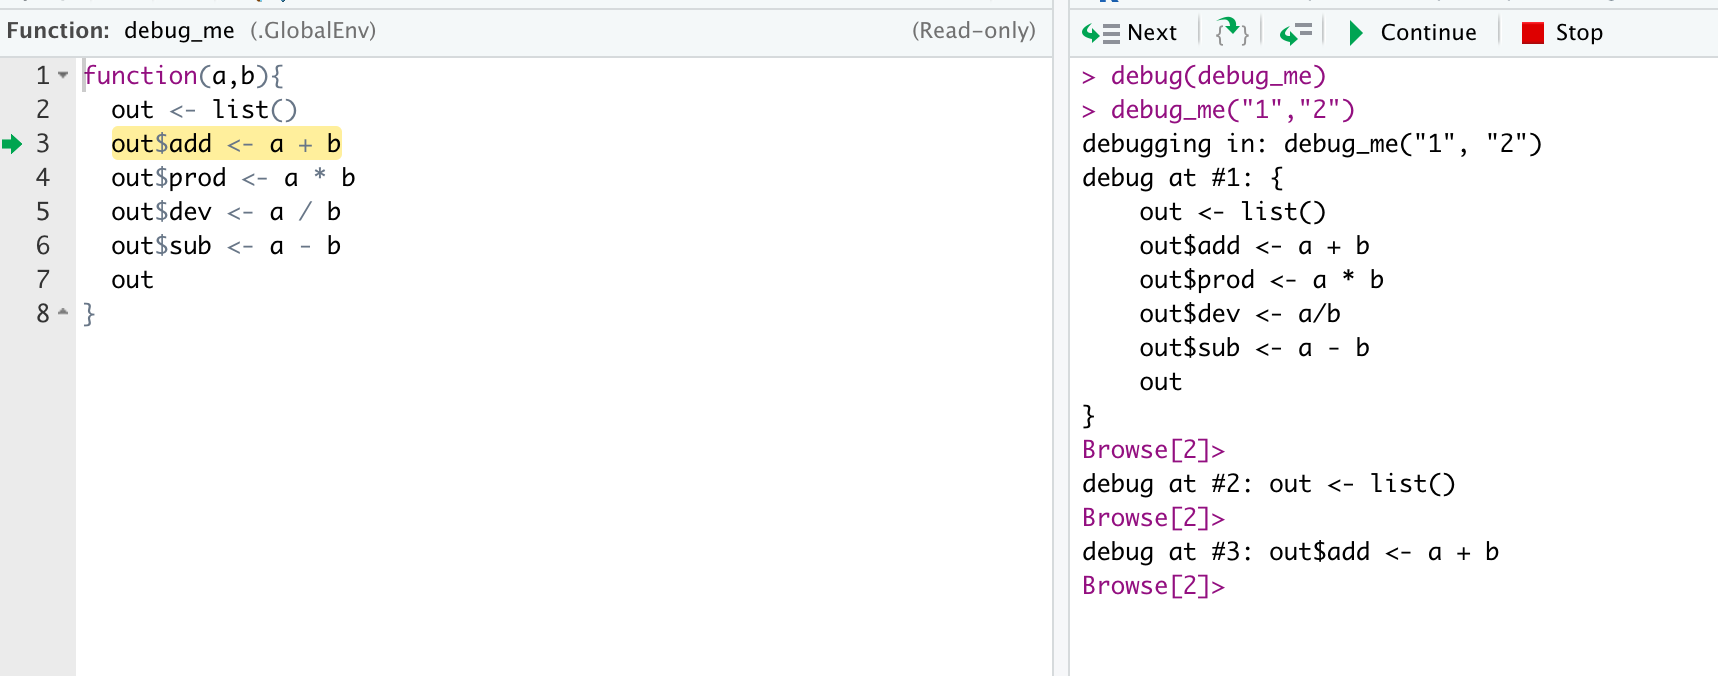
\includegraphics{./images/debug.png}

\hypertarget{a-word-on-peer-programming}{%
\section{A Word on Peer Programming}\label{a-word-on-peer-programming}}

Peer programming, also called pair programming, just means that two
developers sit in front of the same screen to collaborate on a piece of
code. So why is there such a buzz about it? Why is there even a term for
it? And why is there a section in an applied book on it?

That is because novice programmers (and their scientific supervisors)
often doubt the efficiency of two paid persons working at the same
workstation. But programming is not about digging a hole with two
shovels. Particularly not when it comes to building the software basis
or frame of a project.

Working together using one single keyboard and screen or the virtual
equivalent thereof can be highly efficient. The virtual equivalent,
i.e., in fact, using two computers but sharing the screen while in call,
helps tremendously with (a) your concept, (b) your documentation. Plus,
it is a code review at the same time. But most importantly, both
developers learn from each other. Having to explain and being
challenged, deepens the understanding of experienced developers and
ruthlessly identifies holes in one's knowledge. One important advice
when peer programming is to switch the driver's seat from time to time.
Make sure the lesser programmer holds the keys occasionally and
maneuvers through articles, repositories, code and data. Doing so
prevents the co-pilot from taking a back seat and letting the veteran do
the entertainment. Visual Studio Code Live Share\footnote{https://visualstudio.microsoft.com/services/live-share/}
is a great feature for next-level virtual peer programming, as it allows
for two drivers using two cursors.

Of course, there are downsides of the pair programming approach, too.
Also, timing within the lifecycle of a project is an important factor
and not every project is the same fit for this agile method. But given
there are so many approaches, I will leave the back and forth to others.
The goal of this section is to point the reader to a practical approach
that tends to work well in programming with data setups in social
sciences. Googlers Jeff Dean and Sanjay Ghemawat had their fair share of
success, too, according to \emph{The New Yorker's} The Friendship That
Made Google Huge\footnote{https://www.newyorker.com/magazine/2018/12/10/the-friendship-that-made-google-huge}.

\bookmarksetup{startatroot}

\hypertarget{interaction-environment-1}{%
\chapter{Interaction Environment}\label{interaction-environment-1}}

As a kid of the 90s, reading about a new editor or fancy shell coming
out triggers playing Inspector Gadget's tune in my head. To invest a few
fun hours into exploring a new tool that might save me a split second or
two in processes that I run a hundred times daily may not always pay off
by the hour even in a lifetime of programming, but it is totally worth
it in most cases -- at least to me. Repetitive work is tiring and
error-prone, adds to cognitive workload, and shifts focus away from
hard-to-tackle puzzles.

That being said, I am nowhere near the \emph{vim} aficionados whose
jaw-dropping editing speed probably takes thousands of hours to master
and configure, and I would not advise overengineering setting up your
environment. Like often, finding a personal middle ground between
feeling totally uncomfortable outside graphical user interfaces and
editing code at a 100 words per minute is key.

\begin{figure}

{\centering 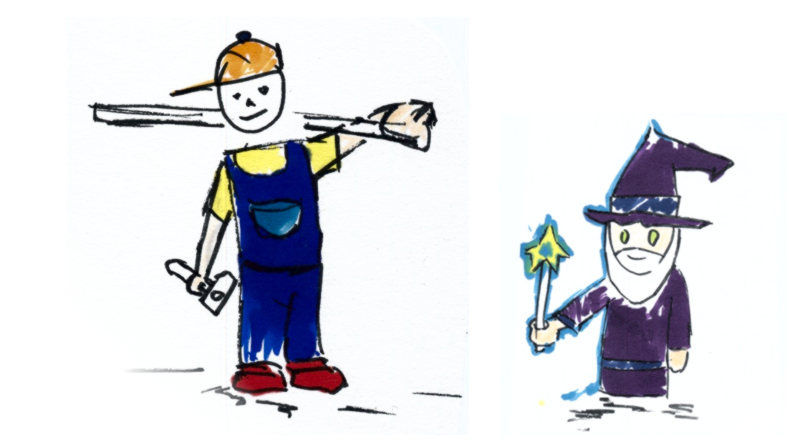
\includegraphics{./images/wizardry.jpg}

}

\caption{Wizard or Carpenter? Aiming at solid mastery of your toolset is
sufficient to become happy with a programming approach to analytics.
(Source: own illustration.)}

\end{figure}

Most likely, investing in an initial setup of a solid editor plus some
basic terminal workflows are a good starting point that can be revisited
every once in a while, e.g., when we start a larger new project. What
editor you will center your environment around will depend a lot on the
programming language you choose. Yet, it also depends on your personal
preference of how much investment, support and supportive features you
want. The following features/criteria are likely the most influential
when composing a programming environment for statistical computing:

\begin{itemize}
\tightlist
\item
  \emph{code highlighting}, i.e., use of colors to highlight the
  structure of your code
\item
  \emph{linting} scans the code for potential errors and displays hints
  in the editor
\item
  integrated \emph{debuggers} allow running parts of the code
  line-by-line and to inspect the inner workings of functions
\item
  \emph{multi-language support} is important when working in multiple
  programming or markup languages.
\item
  \emph{terminal integration} helps to run stuff using system commands
\item
  git integration helps interact with git \index{version control} and do
  basic add, commit, push operations through the editor's GUI
\item
  build tools for programs that need rendering and compilation
\item
  customizable through add-ins/macros
\end{itemize}

\hypertarget{integrated-development-environments}{%
\section{Integrated Development
Environments}\label{integrated-development-environments}}

While some prefer lightning-fast editors such as Sublime Text that are
easy to customize but rather basic out-of-the-box, Integrated
Development Environments\index{IDE} (IDEs) are the right choice for most
people. In other words, it's certainly possible to move a five-person
family into a new home by public transport, but it is not convenient.
The same holds for (plain) text editors in programming. You can use
them, but most people would prefer an IDE just like they prefer to use a
truck over public transport when they move. IDEs are tailored to the
needs and idiosyncrasies of a language, some working with plugins and
covering multiple languages. Others have a specific focus on a single
language or a group of languages.

The below sections will focus on data science' most popular editors,
namely Visual Studio Code and RStudio. Hence, I would like to mention at
least some IDE juggernauts here, for the reader looking for
alternatives: \href{https://www.eclipse.org/}{Eclipse} (mostly Java but
tons of plugins for other languages), or JetBrains'
\href{https://www.jetbrains.com/idea/}{IntelliJ} (Java) and
\href{https://www.jetbrains.com/pycharm/}{PyCharm}
(Python)\index{Python}.

\hypertarget{rstudio}{%
\subsection{RStudio}\label{rstudio}}

Posit's \emph{RStudio} has become the default environment for most R
people and those who mostly use R but C or Python\index{Python} and
Markdown, in addition. The open source version ships for free as RStudio
Desktop and RStudio Server Open Source. In addition, the creators of
RStudio offer commercially supported versions of both the desktop and
server version (Posit Workbench). If you want your environment to
essentially look like the environment of your peers, RStudio is a good
choice. To have the same visual image in mind can be very helpful in
workshops, coaching or teaching.

RStudio has four control panes which the user can fill with a different
functionality like script editor, R console, terminal, file explorer,
environment explorer, test suite, build suite and many others. I advise
newcomers to change the default to have the script editor and the
console next to each other (instead of below each other). That is
because (at least in the Western world) we read from left to right and
send source code from left to right to execute it in the console.
Combine this practice with the \emph{run selection shortcut} (cmd+enter
or ctrl+enter on a PC) and you have gained substantial efficiency
compared to leaving your keyboard, reaching for your mouse and finding
the right button. In addition, this workflow should allow you to see
larger chunks\footnote{Many coding conventions recommend having no more
  than 80 characters in one line of code. Sticking to this convention
  should prevent cutting off your code horizontally.} of your code as
well as your output.

\hypertarget{explore-extensions}{%
\subsubsection*{Explore Extensions}\label{explore-extensions}}
\addcontentsline{toc}{subsubsection}{Explore Extensions}

\begin{itemize}
\item
  explore add-ins
\item
  explore the API
\end{itemize}

\hypertarget{favorite-shortcuts}{%
\subsubsection*{Favorite Shortcuts}\label{favorite-shortcuts}}
\addcontentsline{toc}{subsubsection}{Favorite Shortcuts}

\begin{itemize}
\item
  use cmd+enter (ctrl+enter on PCs) to send selected code from the
  script window (on the left) to the console (on the right)
\item
  cmd+shift+option+R, while the cursor is within a function's body
  (create a Roxygen documentation skeleton)
\item
  use ctrl 1,2 to switch between console and script pane
\end{itemize}

\hypertarget{pitfalls}{%
\subsubsection*{Pitfalls}\label{pitfalls}}
\addcontentsline{toc}{subsubsection}{Pitfalls}

\begin{itemize}
\tightlist
\item
  you may stumble over RStudio's defaults, such as storing your global
  environment on exit and thus resurrecting long forgotten objects
  impacting your next experiment through, e.g., lexical
  scoping\index{lexical scoping}.
\item
  RStudio's git integration abstracts git essentials away, so it hampers
  understanding of what's going on.
\end{itemize}

For R, the Open Source Edition of
\href{https://rstudio.com/products/rstudio/}{RStudio Desktop} is the
right choice for most people. (If you are working in a team, R Studio's
server version is great. It allows having a centrally managed server
which clients can use through their web browser without even installing
R and RStudio locally.) R Studio has solid support for a few other
languages often used together with R, plus it's customizable. The French
premier thinkR \href{https://x.com/_colinfay}{Colin\_Fay} gave a nice
tutorial on
\href{https://speakerdeck.com/colinfay/hacking-rstudio-advanced-use-of-your-favorite-ide}{Hacking
RStudio} at the useR! 2019 conference.

Back in fall 2020, long before RStudio turned into Posit, the company
already indicated that data science was not about R vs.~Python to them
(\href{/programming.html\#the-choice-that-doesnt-matter}{Remember the
first section of Chapter 3 of this book: \emph{The Choice That Doesn't
Matter} of this book?})

\begin{figure}

{\centering 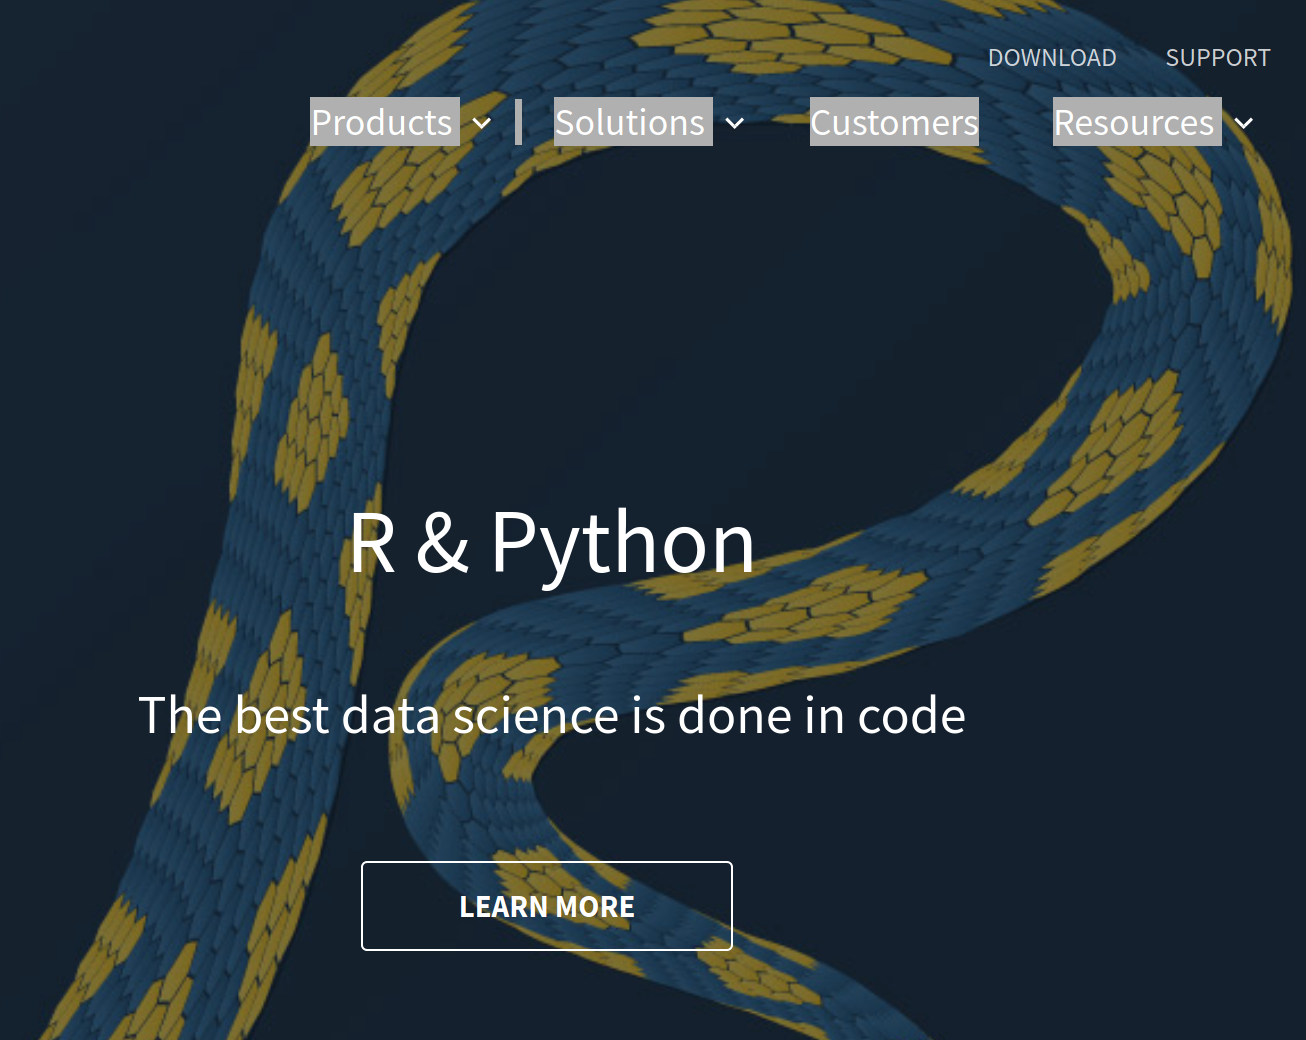
\includegraphics{./images/rstudio_r_py.png}

}

\caption{Called RStudio back then, the company called Posit today
already indicated years ago, it was not solely about R. (Source:
rstudio.com website in 2021)}

\end{figure}

\hypertarget{visual-studio-code}{%
\subsection{Visual Studio Code}\label{visual-studio-code}}

Outside the R universe (and to some degree even inside it), Visual
Studio Code became the go-to editor in data science. Microsoft's Visual
Studio Code started out as a modular, general purpose IDE not focused on
a single language. Meanwhile, there is not only great Python support,
but also auto-completion, code highlighting for R or Julia and many
other languages.
\href{https://visualstudio.microsoft.com/services/live-share/}{VS Code
Live Share} is just one rather random example of its remarkably
well-implemented features. Live share allows developers to edit a
document simultaneously using multiple cursors similarly to Google Docs,
but with all the IDE magic in a Desktop client.

\hypertarget{editors-on-steroids}{%
\subsection{Editors on Steroids}\label{editors-on-steroids}}

Another approach is to go for a highly customizable editor such as
Sublime\footnote{https://www.sublimetext.com/} or Atom\footnote{https://atom.io/}.
The idea is to send source code from the editor to interchangeable
read-eval-print-loop (\protect\hyperlink{glossary}{REPL})s) which can be
adapted according to the language that needs to be interpreted. That way
a good linter/code highlighter for your favorite language is all you
need to have a lightweight environment to run things. An example of such
a customization approach is Christoph Sax's small project Sublime
Studio\footnote{https://github.com/christophsax/SublimeStudio}.

For readers with Unix experience, vim\footnote{https://www.vim.org/} may
just be the most ubiquitous editor of them all, to everyone else it may
just live in deep nerd territory. The fact that a quick online search
for ``How to quit vim'' came back with more than 56.4 million (!)
results shows that both perspectives have a point. With vim, users can
switch between a \emph{move around} and \emph{insert} mode. The former
allows the users to use single letters as shortcuts to navigate a text
file instead of typing the actual letter. This enables users to do
things like move-three-words-forward or delete the next three lines and
many other more complex things. Given some practice and regular use, it
is easy to imagine that vim wizards can navigate their source code
incredibly quickly.\\
Back when IDEs were less comfortable and often clunky due to their heavy
lifting, a broader group of people had their incentives to invest into
vim. Now that IDEs became so much better and many of them even offering
vim modes or plugins, the point of contact with vim for a data scientist
is mostly Unix server administration or work inside
containers\index{container}. GNU Emacs\footnote{https://www.gnu.org/software/emacs/}
is another noteworthy editor because, even though much more exotic, it
is popular among long-tenured R folks thanks to the Emacs Speaks
Statistics extension.

\hypertarget{notebooks}{%
\section{Notebooks}\label{notebooks}}

Notebooks are yet another popular choice for a home court among data
scientists and analysts. Though most often associated with the Python
world\index{Jupyter}, notebooks are language-agnostic and also common
for the R and Julia languages. The basic idea of notebooks is to run web
server in the background to present a browser-based frontend to the
developer. The difference between the Markdown rendering approach
described in \href{publishing.html}{Chapter 10 about publishing} is that
the browser is not just used to display the result, but it is also the
environment to interactively add commands. The resulting workflow, e.g.,
a data analysis in the making feels like a social media timeline:
execute a command, receive a result posted on a web page printed below
the command, again posting a prompt to expect the next command. This way
we get an endless scroll of commands, analysis and descriptive text in
between.

Consider the following example, drawing a basketball court using the
\emph{matplotlib} Python package. This example uses screenshots of a
notebook\index{Jupyter} to illustrate the difference between a notebook
and concepts like RMarkdown. Note the prompts in between the results!

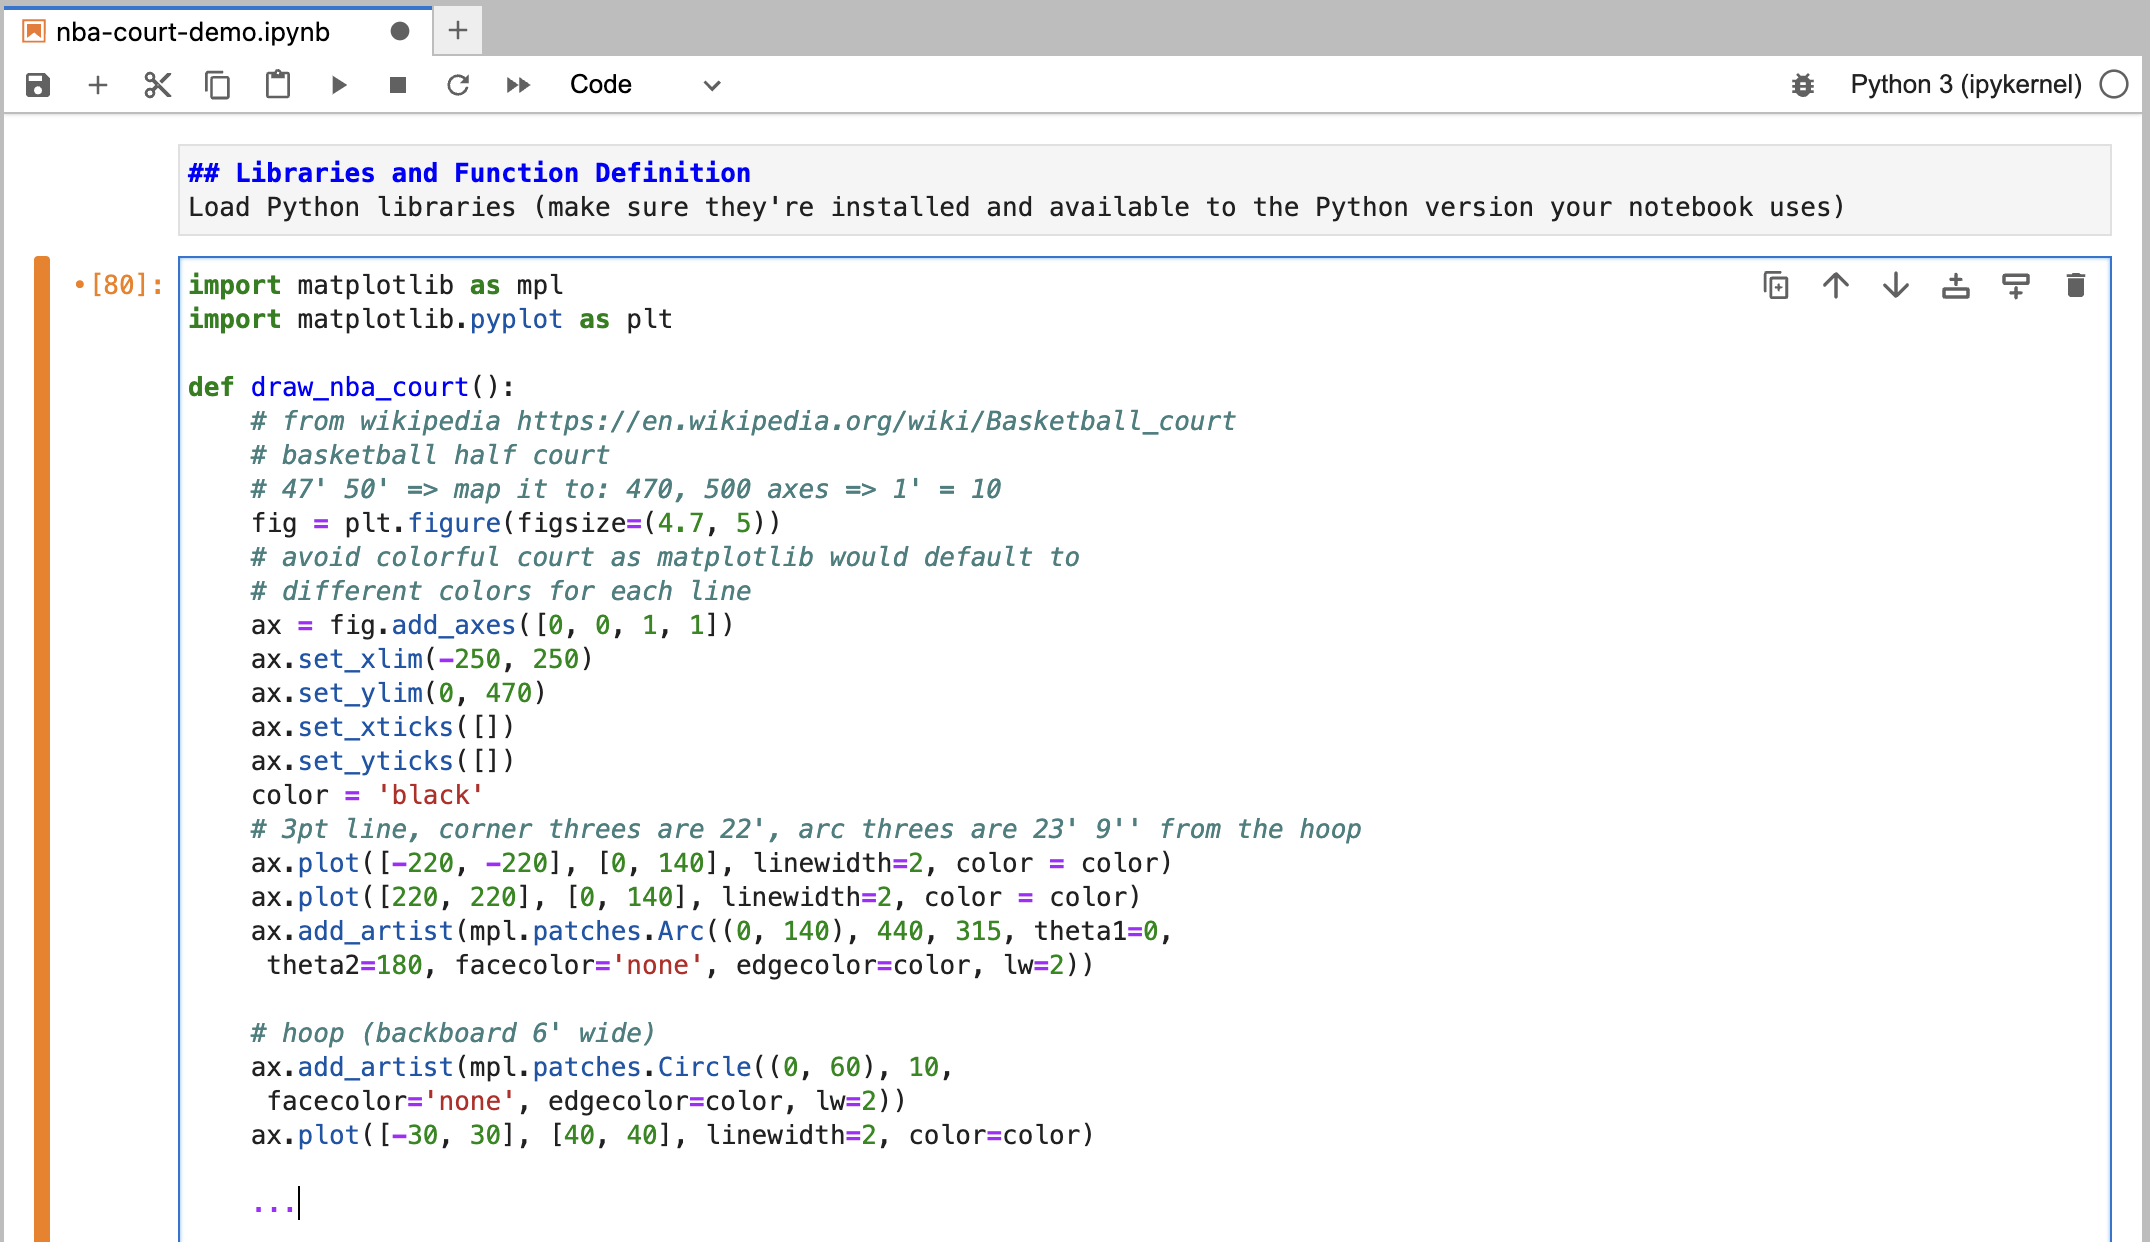
\includegraphics{./images/notebook-1.png}

The above figure depicts a Markdown element in editing mode, showing the
Markdown syntax (double \#\# for a section header of type 2). The second
element is a chunk of Python\index{Python} code to import two well-known
Python libraries.

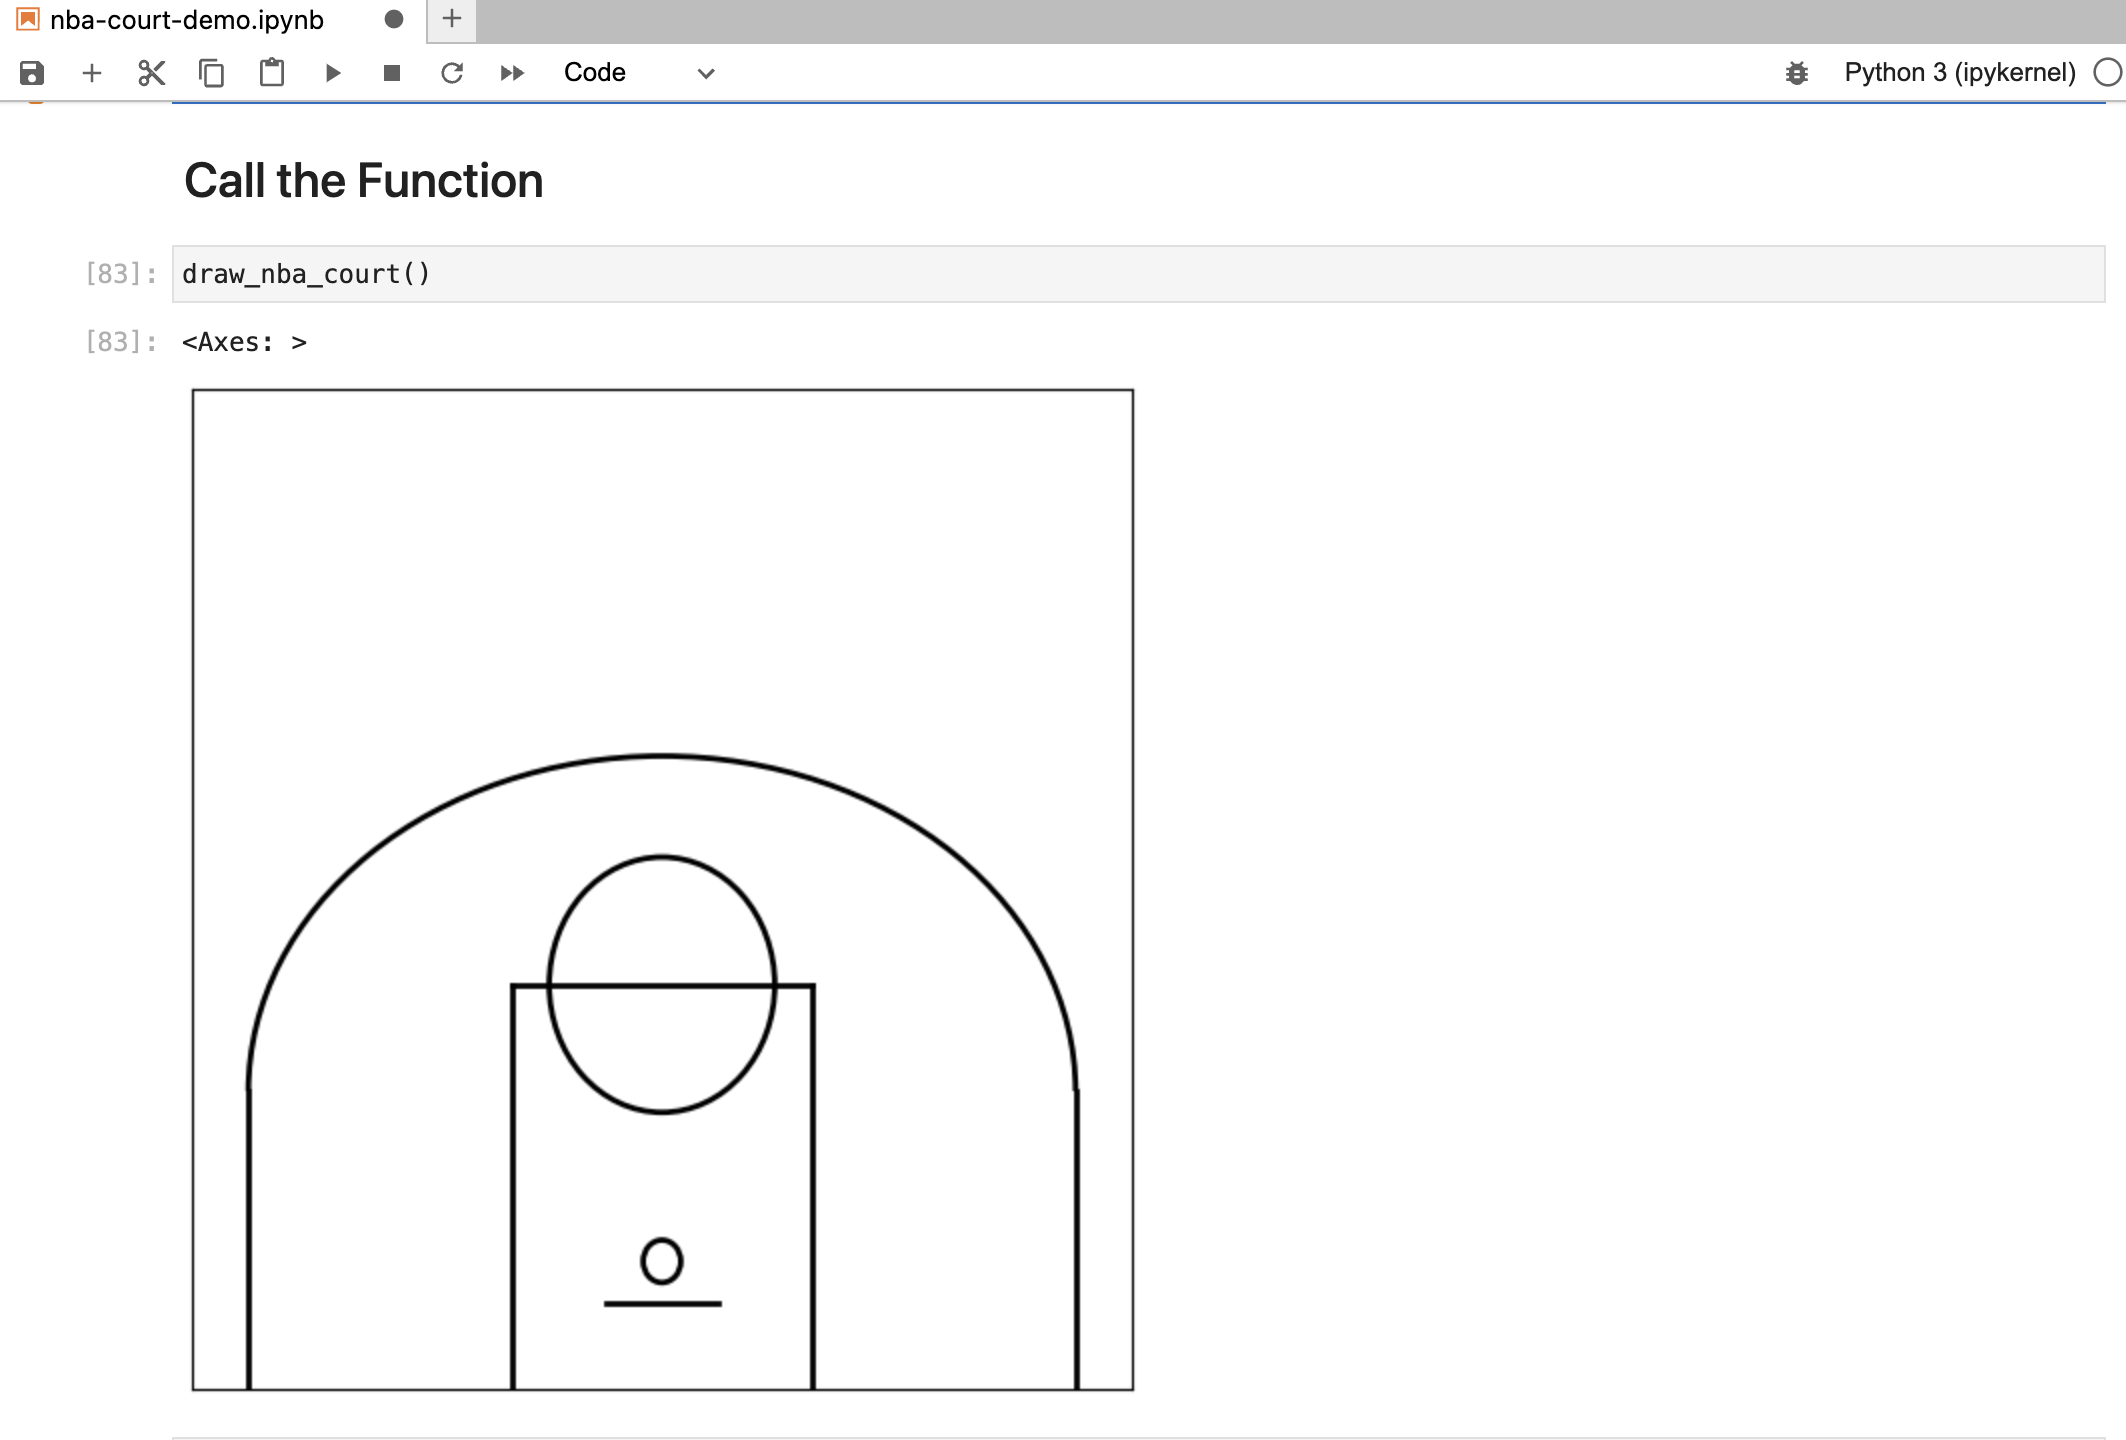
\includegraphics{./images/notebook-2.png}

After the function definition, we see another Markdown section header
element that says \emph{Call the Function} -- this time already rendered
to HTML. Finally, we call the Python\index{Python} function defined
above in another code chunk element\footnote{Though
  notebooks\index{Jupyter} were originally designed to run on a (local)
  Python based webserver and to be used in a web browser, there is a
  neat, Electron-based standalone app called JupyterLab\index{Jupyter}.
  I have used this app for the illustration in this book because of its
  slim, no-nonsense interface that unlike browsers comes without
  distractions from plugins.}.

\hypertarget{consoleterminal}{%
\section{Console/Terminal}\label{consoleterminal}}

In addition to the editor with which you will spend most of your time,
it is also worthwhile to put some effort into configuring
keyboard-driven interaction with your operating systems. And again, you
do not need to be a terminal virtuoso to easily outperform mouse
pushers, a terminal carpentry level is enough. Terminals come in all
shades of gray, integrated into IDEs, built into our operating system or
as pimped third-party applications. A program called a \emph{shell} runs
inside the terminal application to run commands and display output.
\emph{bash} is probably the most known shell program, but there are tons
of different flavors. FWIW, I love \emph{fish}\footnote{https://fishshell.com/}
shell (combined with \emph{iterm2}) for its smooth auto-completion,
highlighting and its extras.

In the Windows world, the use of terminal applications has been much
less common than for OSX/Linux -- at least for non-systemadmins. Git
Bash, which ships with git \index{version control} installations on
Windows, mitigates this shortcoming, as it provides a basic Unix style
console for Windows. For a full-fledged Unix terminal experience, I
suggest using a full terminal emulator like CYGWIN. More recent, native
approaches like powershell brought the power of keyboard interaction at
the OS level to a broader Windows audience --~albeit with different
Windows specific syntax. The ideas and examples in this book as shown in
the below table are limited to Unix flavored shells.

\begin{longtable}[]{@{}
  >{\raggedright\arraybackslash}p{(\columnwidth - 2\tabcolsep) * \real{0.6000}}
  >{\raggedright\arraybackslash}p{(\columnwidth - 2\tabcolsep) * \real{0.4000}}@{}}
\caption{Basic Unix Terminal Commands}\tabularnewline
\toprule()
\begin{minipage}[b]{\linewidth}\raggedright
Command
\end{minipage} & \begin{minipage}[b]{\linewidth}\raggedright
What it does
\end{minipage} \\
\midrule()
\endfirsthead
\toprule()
\begin{minipage}[b]{\linewidth}\raggedright
Command
\end{minipage} & \begin{minipage}[b]{\linewidth}\raggedright
What it does
\end{minipage} \\
\midrule()
\endhead
ls & list files (and directories in a directory) \\
cd & change directory \\
mv & move file (also works to rename files) \\
cp & copy files \\
mkdir & make directory \\
rmdir & remove directory \\
rm -rf & (!) delete everything recursively. DANGER: shell does not ask
for confirmation and just wipes out everything. \\
\bottomrule()
\end{longtable}

\hypertarget{remote-connections-ssh-scp}{%
\subsection{Remote Connections SSH,
SCP}\label{remote-connections-ssh-scp}}

One of the most important use cases of the console for data analysts is
the ability to log into other machines, namely servers that most often
run on Linux. Typically, we use the SSH\index{SSH} protocol to connect
to a (remote) machine that allows to connect through port 22.

\begin{tcolorbox}[enhanced jigsaw, left=2mm, arc=.35mm, colbacktitle=quarto-callout-note-color!10!white, breakable, colframe=quarto-callout-note-color-frame, bottomrule=.15mm, bottomtitle=1mm, colback=white, leftrule=.75mm, coltitle=black, toptitle=1mm, titlerule=0mm, title=\textcolor{quarto-callout-note-color}{\faInfo}\hspace{0.5em}{Note}, opacityback=0, rightrule=.15mm, toprule=.15mm, opacitybacktitle=0.6]

Note that sometimes firewalls limit access to ports other than those
needed for surfing the web (8080 for http:// and 443 for https://) so
you can only access port 22 inside an organization's VPN network.

\end{tcolorbox}

To connect to a server using a username and password, simply use your
console's SSH\index{SSH} client like this:

\begin{Shaded}
\begin{Highlighting}[]
\FunctionTok{ssh}\NormalTok{ mbannert@someserver.org}
\end{Highlighting}
\end{Shaded}

You will often encounter another login procedure, though. SSH\index{SSH}
key pair authentication is more secure and therefore preferred by many
organizations. You need to make sure the public part of your key pair is
located on the remote server and hand the ssh command the private file:

\begin{Shaded}
\begin{Highlighting}[]
\FunctionTok{ssh} \AttributeTok{{-}i}\NormalTok{ \textasciitilde{}/.ssh/id\_rsa mbannert@someserver.org}
\end{Highlighting}
\end{Shaded}

For more details on SSH\index{SSH} key pair authentication, check this
example from the case studies in Chapter 10 Section~\ref{sec-rsa}.

While SSH\index{SSH} is designed to log in to a remote server and from
then on, issue commands like the server was a local Linux machine,
\texttt{scp} copies files from one machine to another.

\begin{Shaded}
\begin{Highlighting}[]
\FunctionTok{scp} \AttributeTok{{-}i}\NormalTok{ \textasciitilde{}/.ssh/id\_rsa \textasciitilde{}/Desktop/a\_file\_on\_my\_desktop}
 \ExtensionTok{mbannert@someserver.org:/some/remote/location/}
\end{Highlighting}
\end{Shaded}

The above command copies a file dwelling on the user's desktop into a
/some/remote/location on the server. Just like SSH\index{SSH}, secure
copy (scp) can use SSH\index{SSH} key pair authentication, too.

\hypertarget{git-through-the-console}{%
\subsection{Git Through the Console}\label{git-through-the-console}}

Another common use case of the terminal is managing git
\index{version control}. Admittedly, there is git integration for many
IDEs that allows you to point and click your way to commits, pushes and
pulls as well as dedicated git clients like GitHub\index{GitHub} Desktop
or Source Tree. But there is nothing like the console in terms of speed
and understanding what you really do. Chapter~\ref{sec-git} sketches an
idea of how to operate git through the console from the very basics to a
feature branch-based workflow.

\bookmarksetup{startatroot}

\hypertarget{sec-git}{%
\chapter{Git Version Control}\label{sec-git}}

As stated before, \index{version control} may be the single most
important thing to take away from \emph{Research Software Engineering}
if you have not used it before. In this chapter about the way developers
work and collaborate, I will stick to \index{version control} with
\emph{git}. The stack\index{stack} discussion of the previous chapter
features a few more \index{version control} systems, but given git's
dominant position, we will stick solely to git in this introduction to
\index{version control}.

\hypertarget{what-is-git-version-control}{%
\section{What Is Git Version
Control?}\label{what-is-git-version-control}}

Git\index{git} is a decentralized version control system. It manages
different versions of your source code (and other text files) in a
simple but efficient manner that has become the industry standard: The
git program itself is a small console program that creates and manages a
hidden folder inside the folder you put under \index{version control}
(you know those folders with a leading dot in their folder name, like
.myfolder). This folder keeps track of all differences between the
current version and other versions before the current one.

\begin{figure}

{\centering 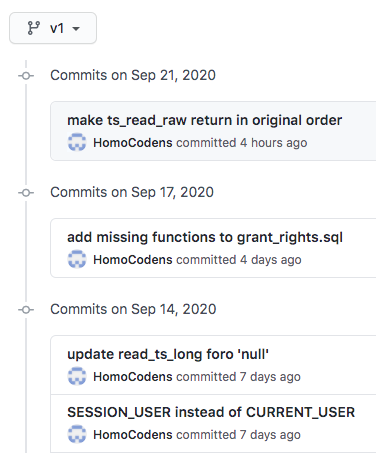
\includegraphics{./images/commits.png}

}

\caption{Meaningful commit messages help to make sense of a project's
history. Screenshot of a commit history on GitHub. Source: (own GitHub
repository.)}

\end{figure}

The key to appreciating the value of git\index{git} is to appreciate the
value of semantic versions. Git is \emph{not} Dropbox nor Google Drive.
It does \emph{not} sync automagically (even if some Git GUI Tools
suggest so). GUI tools GitHub Desktop\footnote{https://desktop.github.com/},
Atlassian's Source Tree\footnote{https://www.sourcetreeapp.com/} and
Tortoise\footnote{https://tortoisegit.org/} are some of the most popular
choices if you are not a console person. Though GUI tools may be
convenient, we will use the git console throughout this book to improve
our understanding. As opposed to the sync approaches mentioned above, a
\index{version control} system allows summarizing a contribution across
files and folders based on what this contribution is about. Assume you
got a cool pointer from an econometrics professor at a conference, and
you incorporated her advice in your work. That advice is likely to
affect different parts of your work: your text and your code. As opposed
to syncing each of these files based on the time you saved them,
\index{version control} creates a version when you decide to bundle
things together and to commit the change. That version could be
identified easily by its commit\index{git commit} message ``incorporated
advice from Anna (discussion at XYZ Conference 2020)''.

\hypertarget{why-use-version-control-in-research}{%
\section{Why Use Version Control in
Research?}\label{why-use-version-control-in-research}}

A \index{version control} based workflow is a path to your goals that
rather consists of semantically relevant steps instead of semantically
meaningless chunks based on the time you saved them.

In other, more blatant, applied words: naming files like
\texttt{final\_version\_your\_name.R} or
\texttt{final\_final\_correction\_collaboratorX\_20200114.R} is like
naming your WiFi \texttt{dont\_park\_the\_car\_in\_the\_frontyard} or
\texttt{be\_quiet\_at\_night} to communicate with your neighbors.
Information is supposed to be sent in a message, not a file name. With
\index{version control}, it is immediately clear what the most current
version is, no matter the file name. There is no room for
interpretation. There is no need to start guessing about the delta
between the current version and another version.

Also, you can easily try out different scenarios on different branches
and merge them back together if you need to. \index{version control} is
a well-established industry standard in software development. And it is
relatively easy to adopt. With datasets growing in complexity, it is
only natural to improve management of the code that processes these
data.

Academia has probably been the only place that would allow you to dive
into hacking at somewhat complex problems for several years without ever
taking notice of \index{version control}. As a social scientist who
rather collaborates in small groups and writes moderate amount of code,
have you ever thought about how to collaborate with more 100 than
persons in a big software project? Or to manage 10,000 lines of code and
beyond? \index{version control} is an important reason these things
work. And it's been around for decades. But enough about the rant.

\hypertarget{how-does-git-work}{%
\section{How Does Git Work?}\label{how-does-git-work}}

This introduction tries to narrow things down to the commands that
you'll need if you want to use git\index{git} in similar fashion to what
you learn from this book. If you are looking for more comprehensive,
general guides, three major git platforms, namely, Atlassian's
Bitbucket\index{Bitbucket}, GitHub\index{GitHub} and
GitLab\index{GitLab} offer comprehensive introductions as well as
advanced articles or videos to learn git online.

The first important implication of decentralized \index{version control}
is that all versions are stored on the local machines of every
collaborator, not just on a remote server (this is also a nice, natural
backup of your work). So let's consider a single local machine first.

\begin{figure}

{\centering 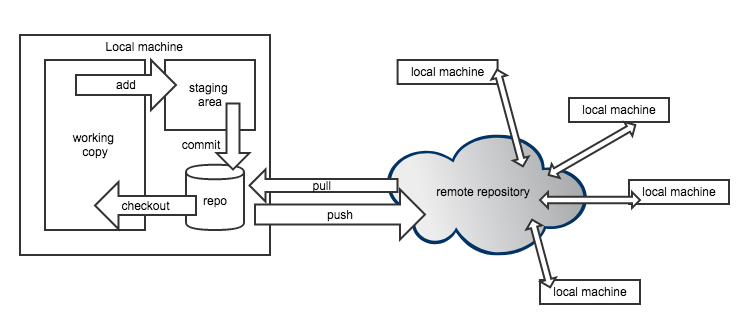
\includegraphics{./images/decentralized.png}

}

\caption{Schematic illustration of an example git workflow including
remote repositories. (Source: own illustation.)}

\end{figure}

Locally, a git repository consists of a \emph{checkout} which is also
called current \emph{working copy}. This is the status of the file that
your file explorer or your editor will see when you use them to open a
file. To check out a different version, one needs to call a commit by
its unique commit hash and check out that particular version.

If you want to add new files to \index{version control} or bundle
changes to some existing files into a new commit, add these files to the
staging area, so they get committed next time a commit process is
triggered. Finally, committing all these staged changes under another
commit ID, a new version is created.

\hypertarget{moving-around}{%
\section{Moving Around}\label{moving-around}}

So let's actually do it. Here's a three-stage walk-through of git
commands that should have you covered in most use cases a researcher
will face. Note that git has some pretty good error messages that guess
what could have gone wrong. Make sure to read them carefully. Even if
you can't make sense of them, your online search will be a lot more
efficient when you include these messages.

\textbf{Stage 1: Working Locally}

Table~\ref{tbl-gitbasics} summarizes essential git
commands\index{git commands} to move around your local repository.

\hypertarget{tbl-gitbasics}{}
\begin{table}
\caption{\label{tbl-gitbasics}Basic Commands for Working with Git }\tabularnewline

\centering
\begin{tabular}{l>{\raggedright\arraybackslash}p{5.7cm}}
\toprule
Command & Effect\\
\midrule
git init & puts current directory and all its subdirs under version control.\\
git status & shows status\\
git add filename.py & adds file to tracked files\\
git commit -m "meaningful msg" & creates a new version/commit out of all staged files\\
git log & shows log of all commit messages on a branch\\
\addlinespace
git checkout some-commit-id & goes to commit, but in detached HEAD state\\
git checkout main-branch-name & leaves temporary state, goes back to last commit\\
\bottomrule
\end{tabular}
\end{table}

\textbf{Stage 2: Working with a Remote Repository}

Though git can be tremendously useful even without collaborators, the
real fun starts when working together. The first step en route to
getting others involved is to add a remote repository.
Table~\ref{tbl-gittable2} shows essential commands\index{git commands}
for working with a remote repository.

\hypertarget{tbl-gittable2}{}
\begin{table}
\caption{\label{tbl-gittable2}Commands for Working with a Remote Repository }\tabularnewline

\centering
\begin{tabular}{>{\raggedright\arraybackslash}p{5.7cm}>{\raggedright\arraybackslash}p{5.7cm}}
\toprule
Command & Effect\\
\midrule
git clone & creates a new repo based on a remote one\\
git pull & gets all changes from a linked remote repo\\
git push & deploys all commit changes to the remote repo\\
git fetch & fetches branches that were created on remote\\
git remote -v & shows remote repo URL\\
\addlinespace
git remote set-url origin https://some-url.com & sets URL to remote repo\\
\bottomrule
\end{tabular}
\end{table}

\textbf{Stage 3: Branches}

Branches are derivatives from the main branch that allow to work on
different features at the same time without stepping on someone else's
feet. Through branches, repositories can actively maintain different
states. Table~\ref{tbl-gitbranches} shows commands\index{git commands}
to navigate these states.

\hypertarget{tbl-gitbranches}{}
\begin{table}
\caption{\label{tbl-gitbranches}Commands for for Handling Multiple Branches }\tabularnewline

\centering
\begin{tabular}{>{\raggedright\arraybackslash}p{5.7cm}>{\raggedright\arraybackslash}p{5.7cm}}
\toprule
Command & Effect\\
\midrule
git checkout -b branchname & creates new branch named branchname\\
git branch & shows locally available branches\\
git checkout branchname & switches to branch named branchname\\
git switch branchname & switches to branch named branchname\\
git merge branchname & merges branch named branchname into current branch\\
\bottomrule
\end{tabular}
\end{table}

\textbf{Fixing Merge Conflicts}

In\index{merge conflict} most cases, \emph{git}\index{git} is quite
clever and can figure out which is the desired state of a file when
putting two versions of it together. When git's \emph{recursive
strategy} is possible, git will merge versions automatically. When the
same lines were affected in different versions, git cannot tell which
line should be kept. Sometimes, you would even want to keep both
changes.

But even in such scenario, fixing the conflict is easy. Git will tell
you that your last command caused a merge conflict and which files are
conflicted. Open these files and see all parts of the file that are in
question.

\begin{figure}

{\centering 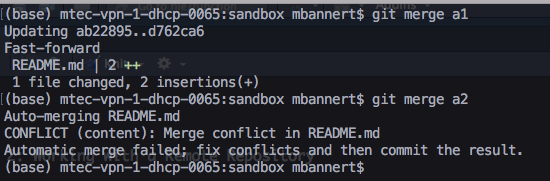
\includegraphics{./images/merge_conflict.png}

}

\caption{Ouch! We created a conflict by editing the same line in the
same file on different branches. Trying merge these branches created a
conflict. (Source: screenshot of own GitHub repository.)}

\end{figure}

Luckily, git marks the exact spot where the
conflict\index{merge conflict} happens. Good text editors/IDEs ship with
cool colors to highlight all our options. Some of the fancier editors
even have git conflict resolve plugins that let you walk through all
conflict points.

\begin{figure}

{\centering 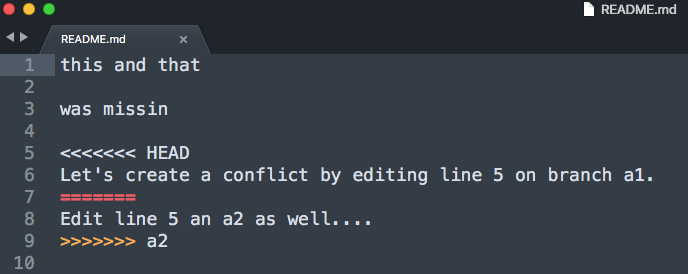
\includegraphics{./images/sublime_conflict.png}

}

\caption{Go for the current status or take what's coming in from the a2
branch? (Source: screenshot of Sublime text editor.)}

\end{figure}

\begin{figure}

{\centering 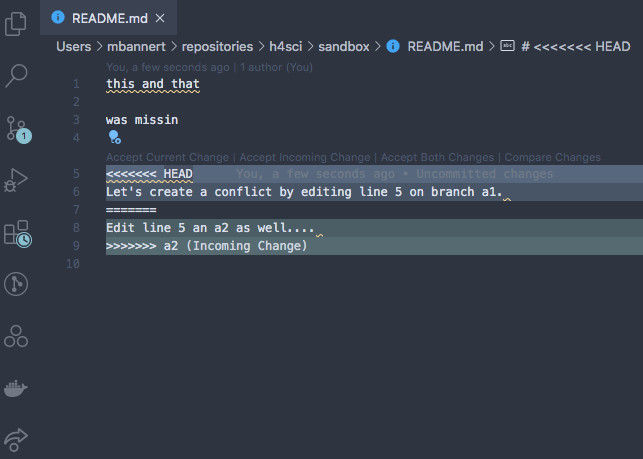
\includegraphics{./images/vscode_conflict.png}

}

\caption{In VS Code, you can even select the option by clicking.
(Source: screenshot VS Code IDE.)}

\end{figure}

At the end of the day, all do the same, i.e., remove the unwanted part,
including all the marker gibberish. After you have done so, save, commit
and push (if you are working with a remote repo) . Don't forget to make
sure you kinked out all conflicts.

\hypertarget{collaboration-workflow}{%
\section{Collaboration Workflow}\label{collaboration-workflow}}

The broad acceptance of git as a framework for collaboration has
certainly played an important role in git's establishment as an industry
standard.

\hypertarget{feature-branches}{%
\subsection{Feature Branches}\label{feature-branches}}

This section\index{feature branch} discusses real-world collaboration
workflows of modern open source software developers. Hence, the
prerequisites to benefitting the most from this section are bit
different. Make sure you are past the mere ability to describe and
explain git basics, make sure you can create and handle your own
repositories.

If you had only a handful of close collaborators so far, you may be fine
with staying on the main branch and trying not to step on each other's
feet. This is reasonable because, git aside, it is rarely efficient to
work asynchronously on exact the same lines of code anyway.
Nevertheless, there is a reason why
\emph{feature-branch-based}\index{feature branch} workflows became very
popular among developers: Imagine yourself collaborating in asynchronous
fashion, maybe with someone in another time zone. Or with a colleague,
who works on your project, but in a totally different month during the
year. Or, most obviously, with someone you have never met. Forks and
\emph{feature-branch-based} workflows are the way a lot of modern open
source projects tackle the above situations.

Forks are just a way to contribute via feature
branches\index{feature branch}, even in case you do not have write
access to a repository. But let's just have a look at the basic feature
branch case, in which you are part of the team first with full access to
the repository. Assume there is already some work done, some version of
the project is already up on a some remote GitHub account. You join as a
collaborator and are allowed to push changes now. It's certainly not a
good idea to simply add things without review to a project's production.
Like if you got access to modify the institute's website, and you made
your first changes and all your changes go straight to production. Like
this:

\textcolor{pink}{It used to be subtle and light gray. I swear!}

Bet everybody on the team took notice of the new team member by then. In
a feature branch workflow, you would start from the latest production
version. Remember, git is decentralized, and you have all versions of
your team's project on your local machine. Create a new branch named
indicative of the feature you are looking to work on.

\begin{verbatim}
git checkout -b colorways
\end{verbatim}

You are automatically being switched to the freshly created branch. Do
your thing now. It could be just a single commit, or several commits by
different persons. Once you are done, i.e., committed all
changes\index{git commands}, add your branch to the remote repository by
pushing.

\begin{verbatim}
git push -u origin colorways
\end{verbatim}

This will add your branch called \emph{colorways} to the remote
repository. If you are on any major git platform with your project, it
will come with a decent web GUI. Such a GUI is the most straightforward
way to do the next step: get your Pull Request\index{pull request} (PR)
out.

\begin{figure}

{\centering 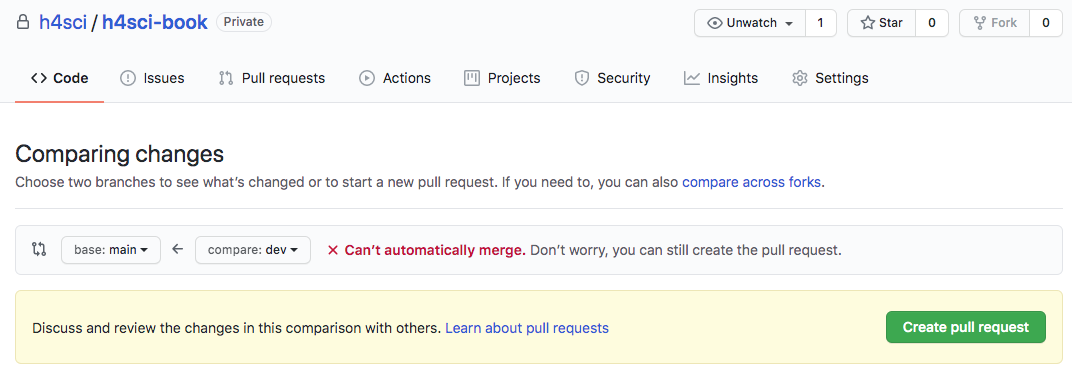
\includegraphics{./images/pr.png}

}

\caption{GitHub\index{GitHub} Pull Request dialog: Select the \emph{Pull
Request}; choose which branch you merge into which target branch.
(Source: own GitHub repository.)}

\end{figure}

As you can see, git will check whether it is possible to merge
automatically without interaction. Even if that is not possible, you can
still issue the pull request\index{pull request}. When you create the
request, you can also assign reviewers, but you could also do so at a
later stage.

Even after a PR\index{pull request} was issued, you can continue to add
commits to the branch about to be merged. As long as you do not merge
the branch through the PR, commits are added to the branch. In other
words, your existing PR gets updated. This is a very natural way to
account for reviewer comments.

\begin{tcolorbox}[enhanced jigsaw, left=2mm, arc=.35mm, colbacktitle=quarto-callout-note-color!10!white, breakable, colframe=quarto-callout-note-color-frame, bottomrule=.15mm, bottomtitle=1mm, colback=white, leftrule=.75mm, coltitle=black, toptitle=1mm, titlerule=0mm, title=\textcolor{quarto-callout-note-color}{\faInfo}\hspace{0.5em}{Note}, opacityback=0, rightrule=.15mm, toprule=.15mm, opacitybacktitle=0.6]

Use commit messages like `added join to SQL\index{SQL}query, closes
\#3'. The keyword `closes' or `fixes', will automatically close issues
referred to when merged into the main branch.

\end{tcolorbox}

Once the merge is done, all your changes are in the main branch, and you
and everyone else can pull the main branch that now contains your new
feature. Yay!

\hypertarget{pull-requests-from-forks}{%
\subsection{\texorpdfstring{Pull Requests\index{pull request} from
Forks}{Pull Requests from Forks}}\label{pull-requests-from-forks}}

Now, let's assume you are using an open source software created by
someone else. At some point, you miss a feature that you feel is not too
hard to implement. After googling and reading up a bit, you realize
others would like to have these features, too, but the original authors
did not find the time to implement it yet. Hence, you get to work.
Luckily, the project is open source and up on GitHub, so you can simply
get your version of it, i.e., \emph{fork} the project to your own GitHub
account (just click the \emph{fork} button and follow the instructions)
.

Now that you have your own version of the software with all the access
rights to modify it, you can implement your feature and push it to your
own remote git repository. Because you forked the repository, your
remote git platform will still remember where you got it from and allows
you to issue a pull request to the original author. The original authors
can now review the pull request\index{pull request}, see the changes,
and decide whether they are fine with the feature and its
implementation.

There may very well be some back and forth in the message board before
the pull requests gets merged. But usually these discussions are very
context-aware and sooner or later, you will get your first pull request
approved and merged. In that case, congratulations -- you have turned
yourself into a team-oriented open source collaborator!

\hypertarget{rebase-vs.-merge}{%
\subsection{\texorpdfstring{Rebase\index{git rebase}
vs.~Merge}{Rebase vs.~Merge}}\label{rebase-vs.-merge}}

Powerful systems often provide more than one way to achieve your goals.
In the case of git, putting together two branches of work -- a very
vital task, is exactly such a case: We can either \emph{merge} or
\emph{rebase} branches.

While \emph{merge} keeps the history intact, \emph{rebase} is a
history-altering command. Though most people are happy with the more
straightforward \emph{merge} approach, a bit of context is certainly
helpful.

Imagine the merge approach as a branch that goes away from the trunk at
some point and then grows alongside the trunk in parallel. In case both
histories become out of sync because someone else adds to the main
branch while you keep adding to the feature branch, you can either merge
or rebase to put the two together.

Sitting on a checkout of the feature branch\index{feature branch}, a
merge of the main branch would simply create an additional merge commit
sequentially after the last commit of the feature branch. This merge
commit contains the changes of both branches, no matter if they were
automatically merged using the standard recursive strategy or through
resolving a merge conflict.

As opposed to that, rebase would move all changes to main to before the
feature branch started, then sequentially add all commits of the feature
branch. That way your history remains linear, looks cleaner and does not
contain artificial merge commits.

So, when should we merge, and when should we rebase? There is no clear
rule to that other than to not use rebase on exposed branches such as
main because you would have a different main branch than other
developers. Rebase can ruin your collaborative workflow, yet it helps to
clean up. In my opinion, merging feature branches is just fine for most
people and teams. So unless you have too many people working on too many
different features at once and are in danger of not being able to move
through your history, simply go with the merge approach. The following
Atlassian tutorial\footnote{https://www.atlassian.com/git/tutorials/merging-vs-rebasing}
offers more insights and illustrations to deepen your understanding of
the matter.

\bookmarksetup{startatroot}

\hypertarget{sec-datamngmnt}{%
\chapter{Data Management}\label{sec-datamngmnt}}

\normalsize

\normalsize

Admittedly, I have said the same thing about Chapter~\ref{sec-git} on
version control, yet \emph{data management} may be the single most
impactful chapter of this book. This may be the case in particular if
you come from an environment that mostly organized data in spreadsheets
shared via e-mail or network drives. To contextualize data and think
about (long-term) data management is a step into a bigger world.

After decades of information engineering and computer science, some
can't help wondering why we have not found one perfect,
one-size-fits-all form of data. In fact, a substantial part of
programming with data deals with transforming data from one form into
another. This chapter intends to give an idea of the aspects of data
management most relevant for data analytics. Hopefully, this chapter
helps the reader to assess how far they wanted to dig into data
management.

\hypertarget{forms-of-data}{%
\section{Forms of Data}\label{forms-of-data}}

In research and analytics, data appear in a plethora of different forms.
Yet, most researchers and business analysts are mainly trained to handle
different flavors of two-dimensional data, as in
\textbf{one-observation-one-row}. Ad hoc studies conducted once result
in \emph{cross-sectional data}\index{cross-sectional}: one line per
observation; columns represent variables. Sensor data, server logs or
forecasts of official statistics are examples of single variable data
observed over time. These single variable, longitudinal data are also
known as \emph{time series\index{time series}}. Multivariate time
series\index{time series}, i.e., multivariable, longitudinal data are
often referred to as \emph{panel data}. In our heads, all of these forms
of data are typically represented as rectangular, two-dimensional
one-line-per-observation, spreadsheet-like tables. Here are a few
easy-to-reproduce examples using popular R demo datasets.

\tiny

\begin{Shaded}
\begin{Highlighting}[]
\NormalTok{h }\OtherTok{\textless{}{-}} \FunctionTok{head}\NormalTok{(mtcars)}
\NormalTok{h}
\end{Highlighting}
\end{Shaded}

\begin{verbatim}
                   mpg cyl disp  hp drat    wt  qsec vs am gear carb
Mazda RX4         21.0   6  160 110 3.90 2.620 16.46  0  1    4    4
Mazda RX4 Wag     21.0   6  160 110 3.90 2.875 17.02  0  1    4    4
Datsun 710        22.8   4  108  93 3.85 2.320 18.61  1  1    4    1
Hornet 4 Drive    21.4   6  258 110 3.08 3.215 19.44  1  0    3    1
Hornet Sportabout 18.7   8  360 175 3.15 3.440 17.02  0  0    3    2
Valiant           18.1   6  225 105 2.76 3.460 20.22  1  0    3    1
\end{verbatim}

\begin{Shaded}
\begin{Highlighting}[]
\FunctionTok{dim}\NormalTok{(h)}
\end{Highlighting}
\end{Shaded}

\begin{verbatim}
[1]  6 11
\end{verbatim}

\normalsize

The above output shows an excerpt of the \emph{mtcars}
\textbf{cross-sectional} dataset with 6 lines and 11 variables.
\emph{Airpassenger} is a \textbf{time series\index{time series}} dataset
represented in an R \emph{ts} object which is essentially a vector with
time-based index attribute.

\normalsize

\begin{Shaded}
\begin{Highlighting}[]
\NormalTok{AirPassengers}
\end{Highlighting}
\end{Shaded}

\begin{verbatim}
     Jan Feb Mar Apr May Jun Jul Aug Sep Oct Nov Dec
1949 112 118 132 129 121 135 148 148 136 119 104 118
1950 115 126 141 135 125 149 170 170 158 133 114 140
1951 145 150 178 163 172 178 199 199 184 162 146 166
1952 171 180 193 181 183 218 230 242 209 191 172 194
1953 196 196 236 235 229 243 264 272 237 211 180 201
1954 204 188 235 227 234 264 302 293 259 229 203 229
1955 242 233 267 269 270 315 364 347 312 274 237 278
1956 284 277 317 313 318 374 413 405 355 306 271 306
1957 315 301 356 348 355 422 465 467 404 347 305 336
1958 340 318 362 348 363 435 491 505 404 359 310 337
1959 360 342 406 396 420 472 548 559 463 407 362 405
1960 417 391 419 461 472 535 622 606 508 461 390 432
\end{verbatim}

\normalsize

Let's create \textbf{a multivariate time series\index{time series}
(panel)} dataset, i.e., multiple variables observed over time:

\normalsize

\begin{Shaded}
\begin{Highlighting}[]
\NormalTok{d }\OtherTok{\textless{}{-}} \FunctionTok{data.frame}\NormalTok{(}\AttributeTok{Var1 =} \FunctionTok{rnorm}\NormalTok{(}\DecValTok{10}\NormalTok{, }\DecValTok{0}\NormalTok{),}
           \AttributeTok{Var2 =} \FunctionTok{rnorm}\NormalTok{(}\DecValTok{10}\NormalTok{, }\DecValTok{10}\NormalTok{),}
           \AttributeTok{Var3 =} \FunctionTok{rnorm}\NormalTok{(}\DecValTok{10}\NormalTok{, }\DecValTok{30}\NormalTok{))}
\NormalTok{multi\_ts }\OtherTok{\textless{}{-}} \FunctionTok{ts}\NormalTok{(d, }\AttributeTok{start =} \FunctionTok{c}\NormalTok{(}\DecValTok{2000}\NormalTok{,}\DecValTok{1}\NormalTok{), }\AttributeTok{frequency =} \DecValTok{4}\NormalTok{)}
\NormalTok{multi\_ts}
\end{Highlighting}
\end{Shaded}

\begin{verbatim}
               Var1      Var2     Var3
2000 Q1  1.02029867  9.314696 29.39139
2000 Q2 -0.25724857  9.717470 29.12891
2000 Q3  0.08499734  8.912356 30.13268
2000 Q4  0.06576464 11.295424 30.21506
2001 Q1 -1.27416319  9.862073 27.39755
2001 Q2 -0.13777737  9.242336 29.21419
2001 Q3 -1.23388183  8.862098 29.79669
2001 Q4 -0.63959271 10.328949 30.05015
2002 Q1  0.68139081 10.504162 29.32984
2002 Q2 -0.94594788 10.443409 29.63181
\end{verbatim}

\normalsize

\begin{tcolorbox}[enhanced jigsaw, colback=white, leftrule=.75mm, breakable, colframe=quarto-callout-note-color-frame, bottomrule=.15mm, arc=.35mm, opacityback=0, rightrule=.15mm, toprule=.15mm, left=2mm]
\begin{minipage}[t]{5.5mm}
\textcolor{quarto-callout-note-color}{\faInfo}
\end{minipage}%
\begin{minipage}[t]{\textwidth - 5.5mm}

\textbf{A Note on Long Format vs.~Wide Format} The above multivariable
time series\index{time series} is shown in what the data science
community calls \emph{wide} format\index{wide format}. In this most
intuitive format, every column represents one variable, time is on the
Y-axis. The counterpart is the so-called \emph{long} format shown below.
The long format\index{long format} is a machine-friendly, flexible way
to represent multi-variable data without altering the number of columns
with more variables.

\end{minipage}%
\end{tcolorbox}

\normalsize

\begin{Shaded}
\begin{Highlighting}[]
\FunctionTok{library}\NormalTok{(tsbox)}
\FunctionTok{ts\_dt}\NormalTok{(multi\_ts)[}\DecValTok{1}\SpecialCharTok{:}\DecValTok{15}\NormalTok{,]}
\end{Highlighting}
\end{Shaded}

\begin{verbatim}
      id       time       value
 1: Var1 2000-01-01  1.02029867
 2: Var1 2000-04-01 -0.25724857
 3: Var1 2000-07-01  0.08499734
 4: Var1 2000-10-01  0.06576464
 5: Var1 2001-01-01 -1.27416319
 6: Var1 2001-04-01 -0.13777737
 7: Var1 2001-07-01 -1.23388183
 8: Var1 2001-10-01 -0.63959271
 9: Var1 2002-01-01  0.68139081
10: Var1 2002-04-01 -0.94594788
11: Var2 2000-01-01  9.31469594
12: Var2 2000-04-01  9.71747031
13: Var2 2000-07-01  8.91235581
14: Var2 2000-10-01 11.29542367
15: Var2 2001-01-01  9.86207339
\end{verbatim}

\normalsize

The ability to transform data from one format into the other and to
manipulate both formats is an essential skill for any data scientist or
data engineer. It is important to point out that the ability to do the
above transformations effortlessly is an absolute go-to skill for people
who want to use programming to run analysis. (Different analyses or
visualizations may require one form or the other and ask for quick
transformation).

Hence, popular data science programming languages offer great toolsets
to get the job done. Mastering these toolboxes is not the focus of this
book. R for Data Science and the Carpentries are good starting points if
you feel the need to catch up or solidify your know-how.

Yet, not all information suits a two-dimensional form. Handling
nested\index{nested data} or unstructured information is one of the
fields where the strength of a programming approach to data analysis and
visualization comes into play. Maps are a common form of information
that is often represented in nested\index{nested data} fashion. For an
example of nested data\footnote{The original GeoJSON file from the
  example can be found at
  https://raw.githubusercontent.com/mbannert/maps/master/ch\_bfs\_regions.geojson.},
let's take a look at the map file and code example case study in
Section~\ref{sec-map}. In memory, i.e., in our R session, the data is
represented in a list that contains multiple list elements and may
contain more lists nested inside.

\normalsize

\begin{Shaded}
\begin{Highlighting}[]
\FunctionTok{library}\NormalTok{(jsonlite)}

\NormalTok{json\_ch }\OtherTok{\textless{}{-}}\NormalTok{ jsonlite}\SpecialCharTok{::}\FunctionTok{read\_json}\NormalTok{(}
  \StringTok{"https://raw.githubusercontent.com/...."}
\NormalTok{)}
\FunctionTok{ls.str}\NormalTok{(json\_ch)}
\end{Highlighting}
\end{Shaded}

\normalsize

\normalsize

\begin{verbatim}
crs : List of 2
 $ type      : chr "name"
 $ properties:List of 1
features : List of 7
 $ :List of 3
 $ :List of 3
 $ :List of 3
 $ :List of 3
 $ :List of 3
 $ :List of 3
 $ :List of 3
type :  chr "FeatureCollection"
\end{verbatim}

\normalsize

Another example of nested but structured data is HTML\index{HTML} or XML
trees obtained from scraping websites. Typically, web scraping
approaches like rvest (Hadley Wickham 2022a) or BeautifulSoup (Zheng,
He, and Peng 2015) parse the hierarchical Document Object Model (DOM)
and turn it into an in-memory representation of a website's DOM. For a
DOM parsing example, see case study Section~\ref{sec-webscrape}.

\hypertarget{representing-data-in-files}{%
\section{Representing Data in Files}\label{representing-data-in-files}}

To create the above examples of different forms of data, it was mostly
sufficient to represent data in memory, in this case within an R
session. As an interpreted language, an R interpreter has to run at all
times when using R. The very same is true for Python. Users of these
languages can work interactively, very much like with a pocket
calculator on heavy steroids. All functions, all data, are in loaded
into a machine's RAM (memory) represented as objects of various classes.
This is convenient, but has an obvious limitation: once the sessions
ends, the information is gone. Hence, we need to have a way to store at
least the results of our computation in persistent fashion.

Just like in office or image editing software, the intuitive way to
store data persistently from a programming language is to store data
into files. The choice of the file format is much less straightforward
in our case, though. The different forms of data discussed above,
potential collaborators and interfaces are factors among others that
weigh into our choice of a file format.

\hypertarget{spreadsheets}{%
\subsection{Spreadsheets}\label{spreadsheets}}

Based on our two-dimensional focused intuition and training,
spreadsheets are the on-disk analog of data.frames, data.tables and
tibbles. Formats like \textbf{.csv} or \textbf{.xlsx} are the most
common way to represent two-dimensional data on disk.\\
On the programming side, the ubiquity of spreadsheets leads to a wide
variety of libraries to parse and write different spreadsheet formats.

\normalsize

\begin{Shaded}
\begin{Highlighting}[]
\ImportTok{import}\NormalTok{ csv}
\ImportTok{import}\NormalTok{ pandas }\ImportTok{as}\NormalTok{ pd}

\NormalTok{d }\OperatorTok{=}\NormalTok{ \{}\StringTok{\textquotesingle{}column1\textquotesingle{}}\NormalTok{: [}\DecValTok{1}\NormalTok{,}\DecValTok{2}\NormalTok{], }\StringTok{\textquotesingle{}column2\textquotesingle{}}\NormalTok{: [}\DecValTok{3}\NormalTok{,}\DecValTok{4}\NormalTok{]\}}
\NormalTok{df }\OperatorTok{=}\NormalTok{ pd.DataFrame(data}\OperatorTok{=}\NormalTok{d)}
\NormalTok{df.to\_csv(}\StringTok{"an\_example.csv"}\NormalTok{, sep}\OperatorTok{=}\StringTok{";"}\NormalTok{,encoding}\OperatorTok{=}\StringTok{\textquotesingle{}utf{-}8\textquotesingle{}}\NormalTok{)}
\end{Highlighting}
\end{Shaded}

\normalsize

Comma-separated values\index{csv} (.csv)\footnote{Note that commas are
  not always necessarily the separator in .csv files. Because of the use
  of commas as decimal delimiters in some regions, columns are also
  often separated by semicolons to avoid conflicts.} are a good and
simple option. Their text-based nature makes .csv files language
agnostic and human-readable through a text editor.

\begin{verbatim}
;column1;column2
0;1;3
1;2;4
\end{verbatim}

Though Excel spreadsheets are a convenient interface to office
environments that offer extras such organization into workbooks, the
simpler .csv format has advantages in machine-to-machine communication
and as an interface between different programming languages and tools.
For example, web visualization libraries such as highcharts or echarts
are most commonly written in JavaScript\index{JavaScript} and can
conveniently consume data from .csv files. The above example .csv file
was written in Python\index{Python} and is now easily read by R.

\normalsize

\begin{Shaded}
\begin{Highlighting}[]
\FunctionTok{library}\NormalTok{(readr)}
\NormalTok{csv }\OtherTok{\textless{}{-}}\NormalTok{ readr}\SpecialCharTok{::}\FunctionTok{read\_csv2}\NormalTok{(}\StringTok{"an\_example.csv"}\NormalTok{)}
\NormalTok{csv}
\end{Highlighting}
\end{Shaded}

\begin{verbatim}
# A tibble: 2 x 3
   ...1 column1 column2
  <dbl>   <dbl>   <dbl>
1     0       1       3
2     1       2       4
\end{verbatim}

\normalsize

\hypertarget{file-formats-for-nested-information}{%
\subsection{File Formats for Nested
Information}\label{file-formats-for-nested-information}}

For many data engineers and developers. JavaScript Object Notation
(JSON)\footnote{https://json.org}\index{JSON} has become the go-to file
format for nested data. Just like with .csv basically every programming
language used in data science and analytics has libraries to serialize
and deserialize JSON (read and write). Though harder to read for humans
than .csv, prettified JSON with a decent highlighting color scheme is
easy to read and gives the human reader a good understanding of the
hierarchy at hand. The added complexity comes mostly from the nested
nature of the data, not so much from the file format.

\normalsize

\begin{Shaded}
\begin{Highlighting}[]
\FunctionTok{library}\NormalTok{(jsonlite)}

\NormalTok{li }\OtherTok{\textless{}{-}} \FunctionTok{list}\NormalTok{(}
  \AttributeTok{element\_1 =} \FunctionTok{head}\NormalTok{(mtcars, }\DecValTok{2}\NormalTok{),}
  \AttributeTok{element\_2 =} \FunctionTok{head}\NormalTok{(iris, }\DecValTok{2}\NormalTok{)}
\NormalTok{)}

\FunctionTok{toJSON}\NormalTok{(li, }\AttributeTok{pretty =} \ConstantTok{TRUE}\NormalTok{)}
\end{Highlighting}
\end{Shaded}

\begin{verbatim}
{
  "element_1": [
    {
      "mpg": 21,
      "cyl": 6,
      "disp": 160,
      "hp": 110,
      "drat": 3.9,
      "wt": 2.62,
      "qsec": 16.46,
      "vs": 0,
      "am": 1,
      "gear": 4,
      "carb": 4,
      "_row": "Mazda RX4"
    },
    {
      "mpg": 21,
      "cyl": 6,
      "disp": 160,
      "hp": 110,
      "drat": 3.9,
      "wt": 2.875,
      "qsec": 17.02,
      "vs": 0,
      "am": 1,
      "gear": 4,
      "carb": 4,
      "_row": "Mazda RX4 Wag"
    }
  ],
  "element_2": [
    {
      "Sepal.Length": 5.1,
      "Sepal.Width": 3.5,
      "Petal.Length": 1.4,
      "Petal.Width": 0.2,
      "Species": "setosa"
    },
    {
      "Sepal.Length": 4.9,
      "Sepal.Width": 3,
      "Petal.Length": 1.4,
      "Petal.Width": 0.2,
      "Species": "setosa"
    }
  ]
} 
\end{verbatim}

\normalsize

The above example shows the first two lines of two different, unrelated
rectangular datasets. Thanks to the hierarchical nature of JSON, both
datasets can be stored in the same file albeit totally different
columns. Again, just like .csv, JSON works well as an interface, but it
is more flexible than the former.

Besides JSON, \textbf{XML} is the most common format to represent nested
data in files. Though there are a lot of overlapping use cases, there is
a bit of a different groove around both of these file formats. JSON is
perceived as more lightweight and close to ``the web'' while XML is the
traditional, very explicit no-nonsense format. XML\index{XML} has a
\textbf{Document Type Definition (DTD)} that defines the structure of
the document and which elements and attributes are legal. Higher level
formats use this more formal approach as XML-based definition.
SDMX\footnote{SDMX (https://sdmx.org)\index{SDMX} stands for Statistical
  Data and Metadata eXchange is an international initiative that aims at
  standardizing and modernizing (``industrializing'') the mechanisms and
  processes for the exchange of statistical data and metadata among
  international organizations and their member countries. SDMX is
  sponsored by seven international organizations including the Bank for
  International Settlements (BIS), the European Central Bank (ECB),
  Eurostat (Statistical Office of the European Union), the International
  Monetary Fund (IMF), the Organisation for Economic Co-operation and
  Development (OECD), the United Nations Statistical Division (UNSD),
  and the World Bank.}, a world-wide effort to provide a format for
exchange statistical data and metadata, is an example of such a higher
level format build on XML.

The above example shows an excerpt of the main economic forward-looking
indicator (FLI) for Switzerland, the KOF Economic Barometer, represented
in an SDMX\index{SDMX} XML\index{XML} file. Besides the value and the
date index, several attributes provide the consumer with an elaborate
data description. In addition, other nodes and their children provide
information like \emph{Contact} or \emph{ID} in the very same file. Note
that modern browsers often provide code folding for nodes and
highlighting to improve readability.

\hypertarget{a-word-on-binaries}{%
\subsection{A Word on Binaries}\label{a-word-on-binaries}}

Unlike all file formats discussed above, binaries cannot be read by
humans using a simple text editor. In other words, you will need the
software that wrote the binary to read it again. If that software was
expensive and/or exotic, your work is much less accessible, more
difficult to share and harder to reproduce. Though this disadvantage of
binaries is mitigated when you use freely available open source
software, storing data in binaries can still be a hurdle.

But, of course, binaries do have advantages, too: binaries can compress
their content and save space. Binaries can take on all sorts of
in-memory objects including functions, not just datasets. In other
words, binaries can bundle stuff. Consider the following load/save
operation in R:

\normalsize

\begin{Shaded}
\begin{Highlighting}[]
\NormalTok{bogus }\OtherTok{\textless{}{-}} \ControlFlowTok{function}\NormalTok{(a,b)\{}
\NormalTok{  a }\SpecialCharTok{+}\NormalTok{ b}
\NormalTok{\} }

\FunctionTok{data}\NormalTok{(Airpassengers)}
\FunctionTok{data}\NormalTok{(mtcars)}

\NormalTok{s }\OtherTok{\textless{}{-}} \FunctionTok{summary}\NormalTok{(mtcars)}

\FunctionTok{save}\NormalTok{(}\StringTok{"bogus"}\NormalTok{, }\StringTok{"Airpassengers"}\NormalTok{,}\StringTok{"s"}\NormalTok{,}
     \AttributeTok{file=}\StringTok{"bundle.RData"}\NormalTok{)}
\end{Highlighting}
\end{Shaded}

\normalsize

In memory, \emph{bogus} is a \emph{function}, Airpassengers is an R
\emph{time series\index{time series}} object and \emph{s} is a
\emph{list} based summary object. All of these objects can be stored in
a single binary RData file using \emph{save()}. A fresh R session can
now \emph{load()} everything stored in that file.

\normalsize

\begin{Shaded}
\begin{Highlighting}[]
\FunctionTok{load}\NormalTok{(}\StringTok{"bundle.RData"}\NormalTok{)}
\end{Highlighting}
\end{Shaded}

\normalsize

\begin{quote}
Notice that unlike reading a .csv or .json file, the call does not make
any assignments into a target object. This is because all objects are
loaded into an R environment (\emph{.globalEnv} by default) with their
original names.
\end{quote}

\hypertarget{interoperable-file-formats}{%
\subsection{Interoperable File
Formats}\label{interoperable-file-formats}}

Interoperable file formats\index{interoperable file formats} cover some
middle ground between the options described above. The
\emph{cross-language in-memory development platform} Apache
Arrow\footnote{https://arrow.apache.org/} is a well-established project
that also implements file formats that work across many popular (data
science) environments. Though the major contribution of the Apache Arrow
project is to allow sharing in-memory data store across environments, I
will just show it as an example for interoperable file formats here.
Nevertheless, if you're interested in a modern, yet established
cross-environment data science project, digging deeper into Apache
Arrow\index{Apache Arrow} is certainly a fun experience.

From the Apache Arrow documentation:

\normalsize

\begin{Shaded}
\begin{Highlighting}[]
\FunctionTok{library}\NormalTok{(dplyr)}
\FunctionTok{library}\NormalTok{(arrow)}
\FunctionTok{data}\NormalTok{(}\StringTok{"starwars"}\NormalTok{)}
\NormalTok{file\_path\_sw }\OtherTok{\textless{}{-}} \StringTok{"starwars.parquet"}
\FunctionTok{write\_parquet}\NormalTok{(starwars, file\_path\_sw)}
\end{Highlighting}
\end{Shaded}

\normalsize

The above R code writes the \emph{starwars} demo dataset from the
\emph{dplyr} R package to a temporary .parquet file. The \{arrow\} R
package (Richardson et al. 2022) comes with the necessary toolset to
write the open source columnar\footnote{see also} .parquet
format\index{Parquet}. Though they are not text files, .parquet files
can be read and written from different environments and consume the file
written with R. The below code uses the arrow library for Python to read
the file we have just written with R.

\normalsize

\begin{Shaded}
\begin{Highlighting}[]
\ImportTok{import}\NormalTok{ pyarrow.parquet }\ImportTok{as}\NormalTok{ pa}
\NormalTok{sw }\OperatorTok{=}\NormalTok{ pa.read\_table(}\StringTok{"starwars.parquet"}\NormalTok{)}
\BuiltInTok{print}\NormalTok{(}\OperatorTok{*}\NormalTok{sw.column\_names, sep}\OperatorTok{=}\StringTok{"}\CharTok{\textbackslash{}n}\StringTok{"}\NormalTok{)}
\end{Highlighting}
\end{Shaded}

\begin{verbatim}
name
height
mass
hair_color
skin_color
eye_color
birth_year
sex
gender
homeworld
species
films
vehicles
starships
\end{verbatim}

\normalsize

Here's Julia reading our Parquet file:

\normalsize

\begin{Shaded}
\begin{Highlighting}[]
\ImportTok{using} \BuiltInTok{Parquet}
\NormalTok{sw }\OperatorTok{=}\NormalTok{ Parquet.}\FunctionTok{File}\NormalTok{(}\StringTok{"starwars.parquet"}\NormalTok{)}
\end{Highlighting}
\end{Shaded}

\begin{verbatim}
Parquet file: starwars.parquet
    version: 2
    nrows: 87
    created by: parquet-cpp-arrow version 9.0.0
    cached: 0 column chunks
\end{verbatim}

\normalsize

When I composed this example, reading and writing \emph{Parquet} files
in different environments, I ran into several compatibility issues. This
shows that the level of interoperability\index{interoperability} is not
the same as the interoperability of text files.

\hypertarget{columnar}{%
\subsubsection{A Note on Overhead}\label{columnar}}

The \emph{parquet} format is designed to read and write files swiftly
and to consume less disk space than text files. Both features can become
particularly relevant in the cloud. Note though that \emph{Parquet}
comes with some overhead, which may eat up gains if datasets are small.
Consider our \emph{starwars} dataset. At 87 rows and 14 columns, the
dataset is rather small.

\normalsize

\begin{Shaded}
\begin{Highlighting}[]
\FunctionTok{library}\NormalTok{(readr)}
\FunctionTok{write\_csv}\NormalTok{(starwars, }\AttributeTok{file =} \StringTok{"starwars.csv"}\NormalTok{)}
\FunctionTok{dim}\NormalTok{(starwars)}
\end{Highlighting}
\end{Shaded}

\begin{verbatim}
[1] 87 14
\end{verbatim}

\begin{Shaded}
\begin{Highlighting}[]
\FunctionTok{round}\NormalTok{(}\FunctionTok{file.size}\NormalTok{(}\StringTok{"starwars.parquet"}\NormalTok{) }\SpecialCharTok{/} 
      \FunctionTok{file.size}\NormalTok{(}\StringTok{"starwars.csv"}\NormalTok{),}
      \AttributeTok{digits =} \DecValTok{2}\NormalTok{)}
\end{Highlighting}
\end{Shaded}

\begin{verbatim}
[1] 1.47
\end{verbatim}

\normalsize

Hence, the overhead of a schema implementation and other meta
information outweighs \emph{Parquet's} compression for such a small
dataset, leading to a \emph{Parquet} file that is almost 1.5 times
larger than the corresponding csv file. Yet, \emph{Parquet} already
turns the tables for the \emph{diamonds} demo dataset from the
\emph{ggplot2} R package, which is by no means a large dataset.

\normalsize

\begin{Shaded}
\begin{Highlighting}[]
\FunctionTok{library}\NormalTok{(ggplot2)}
\FunctionTok{data}\NormalTok{(diamonds)}
\FunctionTok{write\_csv}\NormalTok{(diamonds, }\AttributeTok{file =} \StringTok{"diamonds.csv"}\NormalTok{)}
\FunctionTok{write\_parquet}\NormalTok{(diamonds, }\StringTok{"diamonds.parquet"}\NormalTok{ )}
\FunctionTok{round}\NormalTok{(}\FunctionTok{file.size}\NormalTok{(}\StringTok{"diamonds.parquet"}\NormalTok{) }\SpecialCharTok{/}
      \FunctionTok{file.size}\NormalTok{(}\StringTok{"diamonds.csv"}\NormalTok{),}
      \AttributeTok{digits =} \DecValTok{2}\NormalTok{)}
\end{Highlighting}
\end{Shaded}

\begin{verbatim}
[1] 0.21
\end{verbatim}

\normalsize

The \emph{Parquet} file for the \emph{diamonds} dataset has roughly one
fifth of the size of the corresponding text file. This is a great
example of why there is not one single, perfect, one-size-fits all form
of data that emerged from decades of information engineering. So when
you choose how you are going to represent data in our project, think
about your goals, your most common use or query and a smooth data
transformation strategy for when the use cases or goals change.

\hypertarget{databases}{%
\section{\texorpdfstring{database\index{database}s}{databases}}\label{databases}}

Given the options that file-based approaches provide, what is (a) the
difference and (b) the added value of going for a
database\index{database} to manage data? The front-and-center difference
is the client interface, but there are many more differences and
benefits.

database\index{database} users use a client program and a query language
to send queries written to a database\index{database}. The client sends
these queries to the database\index{database} host and either performs
an operation on the database\index{database} quietly or returns a
result. The most common example of such a query language is the
Structured Query Language (SQL)\index{SQL}. Using such a query language
leads to a standard way of interaction with the data, no matter how the
dataset looks like in terms of dimensions, size
etc.SQL\index{SQL}database\index{database}s have been around much longer
than data science itself, and continue to be inevitable as application
backends and data archives for many use cases.

\normalsize

\begin{Shaded}
\begin{Highlighting}[]
\KeywordTok{SELECT} \OperatorTok{*} \KeywordTok{FROM}\NormalTok{ myschema.demotable}
\end{Highlighting}
\end{Shaded}

\normalsize

The above query would return all rows and all columns from a table
called \emph{demotable} in a schema called \emph{myschema}. Such a query
can easier be sent from a standalone database\index{database} client, a
database\index{database} specific IDE with a built in client such as
DataGrip\footnote{https://www.jetbrains.com/datagrip/} or a programming
language. Given the ubiquity of database\index{database}s most basically
any programming language has native interfaces to the most common
database\index{database}. And if that is not the case, there is the
database\index{database} management system agnostic ODBC standard that
is supported by all majorSQL\index{SQL}database\index{database}s. The
below code shows how to connect from R to PostgreSQL\index{PostgreSQL},
send queries from within R and receive results as R objects.

\normalsize

\begin{Shaded}
\begin{Highlighting}[]
\FunctionTok{library}\NormalTok{(RPostgres)}
\NormalTok{con }\OtherTok{\textless{}{-}} \FunctionTok{dbConnect}\NormalTok{(}
  \AttributeTok{host =} \StringTok{"localhost"}\NormalTok{,}
  \AttributeTok{user =} \StringTok{"bugsbunny"}\NormalTok{,}
  \CommentTok{\# only works within RStudio}
  \AttributeTok{passwd =} \FunctionTok{.rs.AskForPassword}\NormalTok{(}\StringTok{"Enter Pw"}\NormalTok{), }
  \AttributeTok{dbname =} \StringTok{"some\_db\_name"}
\NormalTok{)}

\CommentTok{\# the result is an R data.frame}
\NormalTok{res }\OtherTok{\textless{}{-}} \FunctionTok{dbSendQuery}\NormalTok{(con,}
 \StringTok{"SELECT * FROM myschema.demotable"}\NormalTok{)}

\CommentTok{\# and we can do R things with it}
\CommentTok{\# such as show the first 6 lines.}
\FunctionTok{head}\NormalTok{(res)}
\FunctionTok{dbDisconnect}\NormalTok{(con)}
\end{Highlighting}
\end{Shaded}

\normalsize

Obviously, the above example barely shows the tip of the iceberg, as it
is just meant to illustrate the way we interact with
database\index{database}s as opposed to a file system. To dig a little
deeper into database\index{database}s, I recommend getting a solid
understanding of the basic CREATE, SELECT, INSERT, UPDATE, DELETE,
TRUNCATE, DROP processes as well as basic JOINs and WHERE clauses. Also,
it is helpful to understand the concept of normalization up to the third
normal form.

\begin{figure}

{\centering 
\includegraphics{./images/postgres.png}

}

\caption{The iconic Postgres elephant logo}

\end{figure}

\hypertarget{relational-database-management-systems-rdbms}{%
\subsection{\texorpdfstring{Relational database\index{database}
Management Systems
(RDBMS)}{Relational database Management Systems (RDBMS)}}\label{relational-database-management-systems-rdbms}}

When you need to pick a concrete database\index{database} technology for
your project, the first major choice is whether to go for a relational
system or not. Unless you have a very compelling reason not to, you are
almost always better off with a relational database\index{database}:
Relational database\index{database}s are well established and accessible
from any programming language used in programming with data that one
could think of. In addition, modern RDBMS implementations offer many
non-relational features such as JSON field types and operations.

I would classify the most popular relational database\index{database}
implementations as follows. First, there is
\href{https://www.sqlite.org/index.html}{SQLite}. As the name
suggestions, \emph{SQLite} is a light-weight, stripped down, easy-to-use
and install implementation.

\begin{quote}
SQLite\index{SQLite} is a C-language library that implements a small,
fast, self-contained, high-reliability,
full-featured,SQL\index{SQL}database\index{database} engine. SQLite is
the most used database\index{database} engine in the world. SQLite is
built into all mobile phones and most computers and comes bundled inside
countless other applications that people use every day. -- SQLite.org
\end{quote}

\emph{SQLite} data lives in a single file that the user queries through
the \emph{SQLite\index{SQLite}} engine. Here is an example using that
engine from R.

\normalsize

\begin{Shaded}
\begin{Highlighting}[]
\FunctionTok{library}\NormalTok{(RSQLite)}
\NormalTok{db\_path }\OtherTok{\textless{}{-}} \StringTok{"rse.sqlite3"}
\NormalTok{con }\OtherTok{\textless{}{-}} \FunctionTok{dbConnect}\NormalTok{(RSQLite}\SpecialCharTok{::}\FunctionTok{SQLite}\NormalTok{(), db\_path)}
\FunctionTok{dbWriteTable}\NormalTok{(con, }\FunctionTok{dbQuoteIdentifier}\NormalTok{(con,}\StringTok{"mtcars"}\NormalTok{),}
\NormalTok{             mtcars, }\AttributeTok{overwrite =}\NormalTok{ T)}
\FunctionTok{dbWriteTable}\NormalTok{(con, }\FunctionTok{dbQuoteIdentifier}\NormalTok{(con,}\StringTok{"flowers"}\NormalTok{),}
\NormalTok{             iris, }\AttributeTok{overwrite =}\NormalTok{ T)}
\end{Highlighting}
\end{Shaded}

\normalsize

The above code initiates a \emph{SQLite\index{SQLite}}
database\index{database} and continues to write the built-in R demo
datasets into separate tables in that newly created
database\index{database}. Now we can useSQL\index{SQL}to query the data.
Return the first three rows of \emph{flowers}:

\scriptsize

\begin{Shaded}
\begin{Highlighting}[]
\FunctionTok{dbGetQuery}\NormalTok{(con, }\StringTok{"SELECT * FROM flowers LIMIT 3"}\NormalTok{)}
\end{Highlighting}
\end{Shaded}

\begin{verbatim}
  Sepal.Length Sepal.Width Petal.Length Petal.Width Species
1          5.1         3.5          1.4         0.2  setosa
2          4.9         3.0          1.4         0.2  setosa
3          4.7         3.2          1.3         0.2  setosa
\end{verbatim}

\normalsize

Return cars that are more fuel efficient than 30 miles per gallon:

\scriptsize

\begin{Shaded}
\begin{Highlighting}[]
\FunctionTok{dbGetQuery}\NormalTok{(con, }\StringTok{"SELECT * FROM mtcars WHERE mpg \textgreater{} 30"}\NormalTok{)}
\end{Highlighting}
\end{Shaded}

\begin{verbatim}
   mpg cyl disp  hp drat    wt  qsec vs am gear carb
1 32.4   4 78.7  66 4.08 2.200 19.47  1  1    4    1
2 30.4   4 75.7  52 4.93 1.615 18.52  1  1    4    2
3 33.9   4 71.1  65 4.22 1.835 19.90  1  1    4    1
4 30.4   4 95.1 113 3.77 1.513 16.90  1  1    5    2
\end{verbatim}

\normalsize

MySQL\footnote{https://www.mysql.com/}\index{MySQL} can do a little more
and is also immensely popular, particularly as a
database\index{database} backend for web content management systems and
other web-based applications. The so-called LAMP stack\index{stack}
(Linux, Apache, MySQL and PHP) contributed to its rise decades ago when
it fueled many smaller and medium-level web projects around the world.
In its early days, MySQL used to be an independent open source project,
but it was later on acquired by database\index{database} Juggernaut
Oracle as a light version to go with its flagship product.

While certainly doing its job in millions of installations, MySQL is not
in at the same level as {[}Microsoft SQL
Server\index{SQL Server}\footnote{https://www.microsoft.com/en-us/sql-server/sql-server-2019}
(MSSQL), PostgreSQL\footnote{https://www.postgresql.org/}\index{PostgreSQL}
and Oracle database\index{database}\footnote{https://www.oracle.com/database\index{database}/technologies/},
and I suggest one of these three enterprise-level
database\index{database}s as a data store for research projects that go
beyond hosting\index{hosting} a blog. Especially when it comes to
long-term conservation of data and enforcing consistency,
MSSQL\index{SQL Server}, PostgreSQL\index{PostgreSQL} and
Oracle\index{Oracle} are hard to beat. Among the three, personally I
would always lean toward the license cost free open source PostgreSQL,
but fitting into existing ecosystems is a good reason to go with either
MSSQL or Oracle if you can afford the licenses. For many use cases,
there is hardly any difference for the analyst or scientific end user.
PostgreSQL may have the coolest spatial support, MSSQL T-SQL dialect,
may have some extra convenient queries if your developers mastered the
dialect and Oracle may have the edge in performance and Java interaction
here and there, but none of these systems is a bad choice.

Another database\index{database} management that gets a lot of attention
recently (and rightfully so) is DuckDB\footnote{https://duckdb.org/}.
Because it is mentioned so positively and often, it is important to
understand what it is and when to use it. DuckDB is not yet another
competitor that tries to gain some ground from the big three of MSSQL,
PostgreSQL and Oracle. DuckDB does offer anSQL\index{SQL}interface, but
it is very different in its aims from the
traditionalSQL\index{SQL}database\index{database}s. DuckDB\index{DuckDB}
is serverless and allows accessing \emph{Parquet}\index{Parquet} files
via a very fastSQL\index{SQL}interface. This makes DuckDB a great tool
for interactive analysis and transfer of large result sets, but it is
not so suitable for enterprise data warehousing.

\hypertarget{a-word-on-non-relational-databases}{%
\subsection{\texorpdfstring{A Word on Non-Relational
database\index{database}s}{A Word on Non-Relational databases}}\label{a-word-on-non-relational-databases}}

Among other things, relational database\index{database}s are ACID
(Atomicity, Consistency, Isolation, and Durability) compliant and ask
for very little in return to provide us with a framework to keep our
data quality high for decades. So unless, you have a very specific use
case that translates to a compelling reason to use a non-relational
database\index{database} stick to SQL. Document-oriented storage or very
unstructured information could be such a reason to use non-relational
database\index{database}s, yet their JSON support allows to also handle
JSON in database\index{database} cells. About a decade ago,
mongoDB\footnote{https://www.mongodb.com/} gained traction, partly
piggybacking the success of JavaScript and server-side JavaScript in
particular. In web development, the MEAN (mongoDB, expressjs, angular
and node) stack\index{stack} become popular, and, with the bundle, the
idea of non-relational database\index{database}s as fast track to a
backend spread.

Columnar stores, which are also considered non-relational, are
conceptionally similar to relational database\index{database}s, though
denormalized and designed to structure sparse data.
database\index{database} systems like Apache Cassandra\footnote{https://cassandra.apache.org/}
are designed to scale horizontally and be highly available, managing
massive amounts of data. Cloud applications that distribute data across
multiple nodes for high availability benefit from such an approach.
Other options include Redis\footnote{https://redis.io/} or
Couchbase\footnote{https://www.couchbase.com/}. If you are not happy
with the ``beyond-the-scope-of-this-book'' argument, blogging experts
like Lukas Eder\footnote{https://blog.jooq.org/tag/nosql/} maybe biased
but much better educated (and fun) to educate you here.

\hypertarget{non-technical-aspects-of-managing-data}{%
\section{Non-Technical Aspects of Managing
Data}\label{non-technical-aspects-of-managing-data}}

The fact that we can do more data work single-handedly than ever before
does not only equate to more options. It also means we need to be aware
of new issues and responsibilities. Those responsibilities range from
leading by example when it comes to etiquette and ethical aspects, to
sticking to privacy rules and complying with security standards. In
addition, to normative restrictions that come with handling data, the
options and choices of data dissemination are a realm of their own. Just
like software publications, you should not just ``drop'' data without a
license and instructions on acceptable use of the data.

\hypertarget{etiquette}{%
\subsection{Etiquette}\label{etiquette}}

Just because content is publicly available on a website does not
automatically mean that bulk downloads, aggregation and republishing are
ok. For example, the ability to scrape a website daily and doing so with
good intent for science does not mean a website's Acceptable Use Policy
(AUP) allows to systematically archive its content.

\begin{tcolorbox}[enhanced jigsaw, colback=white, leftrule=.75mm, breakable, colframe=quarto-callout-important-color-frame, bottomrule=.15mm, arc=.35mm, opacityback=0, rightrule=.15mm, toprule=.15mm, left=2mm]
\begin{minipage}[t]{5.5mm}
\textcolor{quarto-callout-important-color}{\faExclamation}
\end{minipage}%
\begin{minipage}[t]{\textwidth - 5.5mm}

Be responsible when scraping data from websites by following polite
principles: introduce yourself, ask for permission, take slowly and
never ask twice. -- CRAN description of the \{polite\} R package
(Perepolkin 2023).

\end{minipage}%
\end{tcolorbox}

In other words, the new type of researcher discussed in this book needs
to be aware of potential legal and social consequences. The \{polite\} R
package quoted above is an example of an alternative approach that
favors etiquette over hiding IP addresses to avoid access denial.

\hypertarget{security}{%
\subsection{\texorpdfstring{Security\index{Security}}{Security}}\label{security}}

\begin{quote}
I ain't got nothing to hide. I don't care about people reading my stuff.
-- an argument I have heard about a zillion times.
\end{quote}

People who argue like that do not only endanger their environment, they
also contribute to a less secure internet at large, as they leave their
device open to contribute to malicious activity. It does not have to be
you who has been trusted to work with data that qualify as sensitive.
Someone on your team or within your network might have been, and that
person may trust you more than a stranger and may be less vigilant when
harmful actions are executed in your name. This is why you are
\emph{obliged} to care about security. As in, do \emph{not} store your
credentials in your scripts. As in, passwords are \emph{not} part of
your analysis. You may accidentally push your password to GitHub, where
it is not only publicly available but also hard to truly delete for
beginners. Make sure to choose secure passwords. Use a password manager,
so the passwords do not need to be your cat's name for you to remember.
Also, with a password manager you can afford \emph{not} to have the same
passwords for multiple applications. Use a password manager so you can
afford to change your passwords. Use key files where you can. The case
study chapter gives you a hands-on recipe to use RSA key pairs to
connect to remote servers, e.g., your GitHub account instead of a
username/password combination. This is also a good way to connect to a
remote server via SSH\index{SSH}.

In addition to the above Brainy Smurf advice, let me mention
security\index{security} as a reason to consider using a
database\index{database} to manage and archive your data for the long
haul. Enterprise-level database\index{database}s allow for granular
access management and help to stay ahead of users and their rights
regarding your database\index{database}'s entries.

\hypertarget{privacy}{%
\subsection{\texorpdfstring{Privacy\index{privacy}}{Privacy}}\label{privacy}}

Privacy in data science is a complex issue and could legitimately fill a
book on its own. Though I cannot comprehensively cover privacy in a
section, it is important to me to raise awareness and hopefully create
an entry point to the matter. When working with data, in its essence,
respecting privacy is about avoiding exposure of individual units
without their explicit prior consent. It is important to understand that
exposure does not stop at names. A single extraordinary feature or an
exotic combination of features can identify an individual within a
dataset, or at least expose a group. This is why merging multiple
datasets may also cause privacy concerns when datasets were not created
to be merged in the first place, and/or individuals were not aware that
merging was possible. So, what can we as researchers learn from here,
except from concerns and further complication of our work? First,
licenses and usage policies are a service to users of the data. Second,
awareness of what is sensitive data is a valuable skill to have on a
team. That being said, management of in-depth knowledge is rather easy
to organize in a centralized fashion. Most universities and larger
corporations will have an officer to run these things by.

\hypertarget{data-publications}{%
\subsection{Data Publications}\label{data-publications}}

Yet, there is more to managing your data's exposure than just making
sure everything is encrypted and locked up. Publication of data makes
your results reproducible and improves trust in said results. As a
consequence, there is a notable crescendo in the claim for reproducible
research. While reproducible research is great, I would like to raise
awareness that essentially all solutions created and advertised to
improve reproducibility implicitly assume the researcher deals with
datasets obtained through a study. In other words, it is implied that
your work is not about monitoring an ongoing process.

\hypertarget{data-archives}{%
\subsubsection*{Data Archives}\label{data-archives}}
\addcontentsline{toc}{subsubsection}{Data Archives}

Research repositories like Zenodo\footnote{https://zenodo.org}\index{Zenodo}
that allow to archive data follow a snapshot thinking: A catalog entry
refers to a particular version of an research paper, report, software or
dataset. Whenever there is an update, a new version is added to a
catalog entry. Adding datasets or software publications to catalogs like
Zenodo does not only improve reproducibility, it also helps data workers
get credit for their contribution. Fortunately, feeding research
repositories is a task that is easy to automate thanks to
\protect\hyperlink{datapub}{great integration, APIs and community work}.

\hypertarget{open-data}{%
\subsubsection*{Open Data}\label{open-data}}
\addcontentsline{toc}{subsubsection}{Open Data}

Open Data\index{Open Data} archives are a special form of repositories.
The term ``open data'' refers to publicly available data that are
available free of license costs and in machine-readable fashion.

\begin{quote}
``Open data and content can be freely used, modified, and shared by
anyone for any purpose'' -- opendefinition.org
\end{quote}

Because of approaches such as the Swiss government's ``open by
default,'' open government data (OGD) has become a common form of open
data. The basic idea that data generated from publicly funded processes
should be publicly available whenever no privacy rights are violated has
been the motor for many OGD projects out of public administration. From
small local governments to international organizations like the World
Bank or OECD, open data have become a valuable and growing source for
researchers. Open data initiatives of your country, as well as major
international organizations, will help you to create interoperable
datasets. In addition, open data organizations provide you with a
publication channel for your data or with a data catalog that stores the
data description. Initiatives like SDMX (Statistical Data and Meta
eXchange)\footnote{https://sdmx.org/}\index{SDMX} aim to improve
exchange of data \emph{and} data descriptions. Their XML-based format
has become an international standard which led to the implementation of
SDMX read and write routines in statistical software. Whether you think
about the conditions of your own data publications or about a source for
your own research project, make sure to consider open data. The
\emph{openwashdata} project I have been contributing to might be an
hands-on inspiration to get a more concrete understanding of what open
data is actually about. Among other things, the openwashdata project
collects datasets from publications and republishes them in machine
readable format alongside their meta information. The data manipulation
to reach this end is documented in reproducible fashion. The final
results, R data packages, are published in freely available git
repositories in the project's GitHub\index{GitHub} organization.

\begin{quote}
openwashdata is an active global community that applies FAIR
principles\index{FAIR principles} to data generated in the greater
water, sanitation, and hygiene (WASH) sector -- openwashdata.org
\end{quote}

\bookmarksetup{startatroot}

\hypertarget{infrastructure-1}{%
\chapter{Infrastructure}\label{infrastructure-1}}

Yes, there is a third area besides your research and carpentry-level
programming that I suppose you should get an idea about. Again, you do
not have to master hosting servers or even clusters, but a decent
overview and an idea of when to use what will help you tremendously to
plan ahead.

\begin{figure}

{\centering 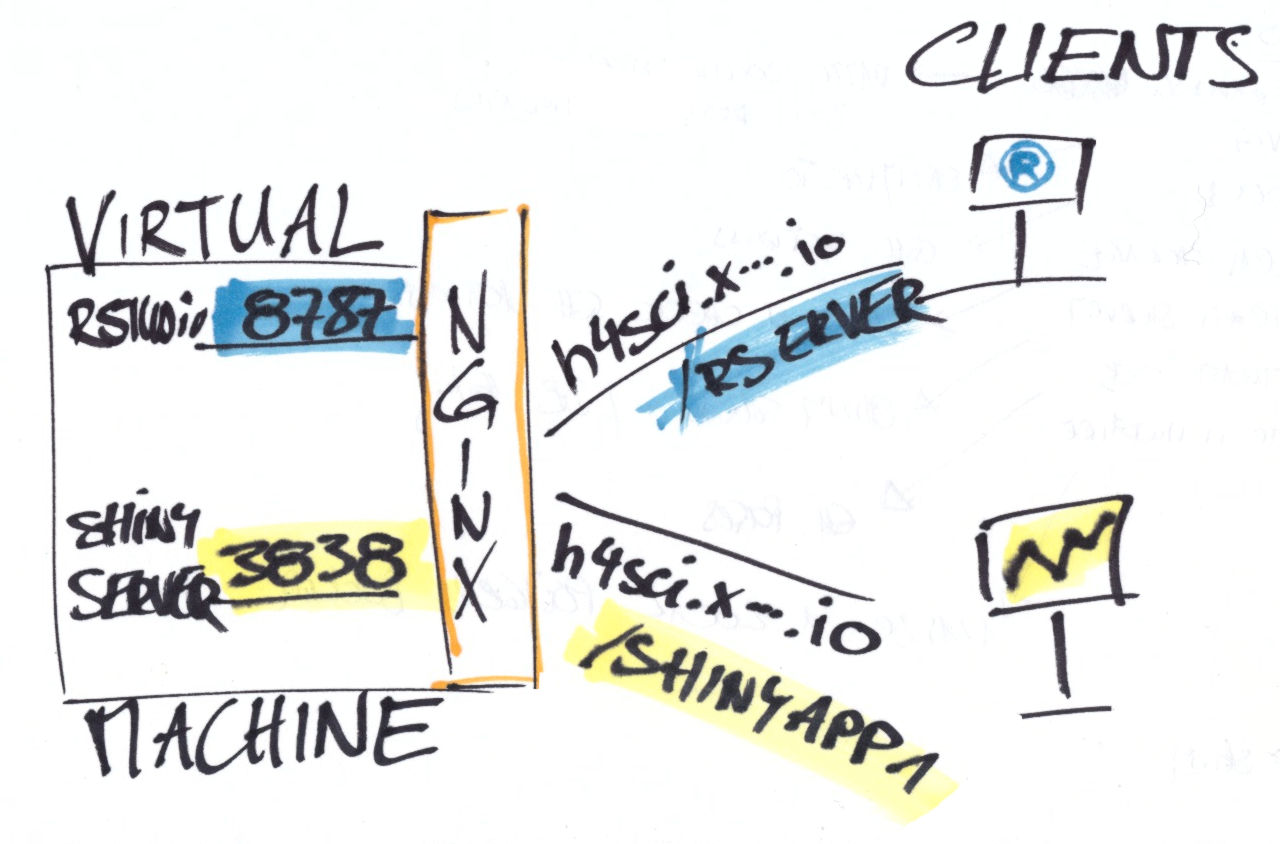
\includegraphics{./images/server-setup3.jpg}

}

\caption{Schematic illustration of a simple server setup for web-based
IDE and web application server. The setup would work well with virtual
machines as well as with docker\index{Docker} containers. (Source: own
illustration.)}

\end{figure}

\hypertarget{why-go-beyond-a-local-notebook}{%
\section{Why Go Beyond a Local
Notebook?}\label{why-go-beyond-a-local-notebook}}

Admittedly, unless you just always had a knack for Arduinos, Raspberry
Pis or the latest beta version of the software you use,
infrastructure\index{infrastructure} may be the one area you perceive as
distracting, none-of-your-business overhead. So, why leave the peaceful,
well-known shire of our local environment for the uncharted, rocky
territory of unwelcoming technical documentations and time-consuming
rabbit holes?

\begin{figure}

{\centering 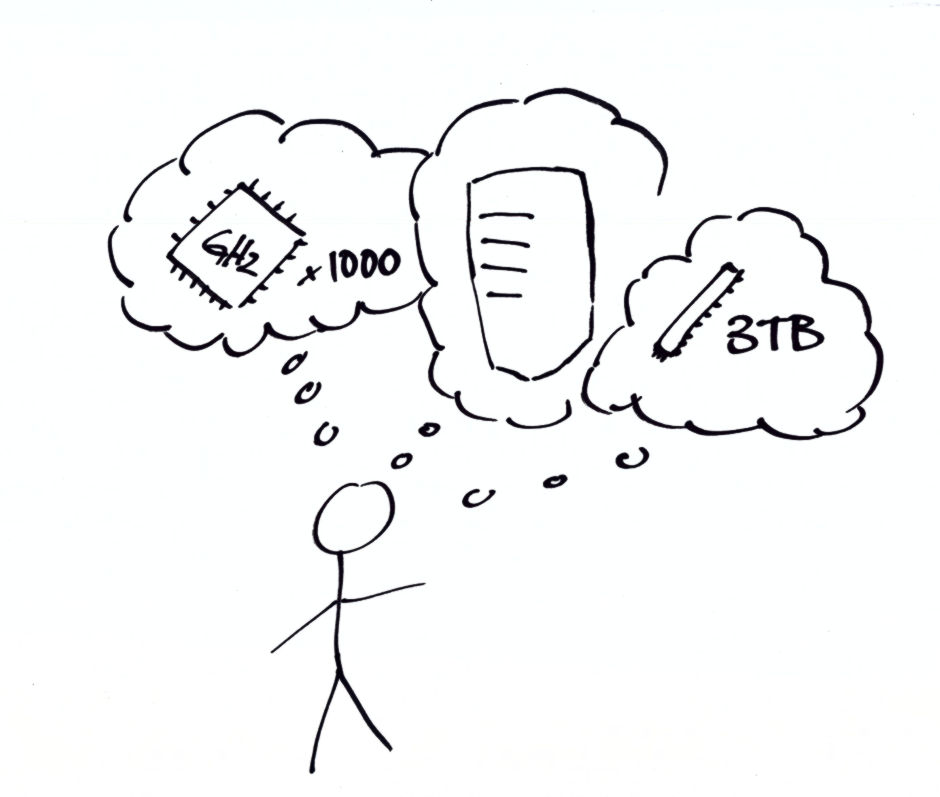
\includegraphics{./images/server-thinking.jpg}

}

\caption{Though servers can provide access to massive computing
resources, do not think of them as a data vault that looks like a
fridge. (Source: own illustration.)}

\end{figure}

Performance, particularly in terms of throughput, is one good reason to
look beyond desktop computers. Data protection regulations that prohibit
data downloads may simply force us to not work locally. Or we just do
not want a crashing office application to bring down a computation that
ran for hours or even days. Or we need a computer that is online 24/7 to
publish a report, website or data visualization.

\begin{figure}

{\centering 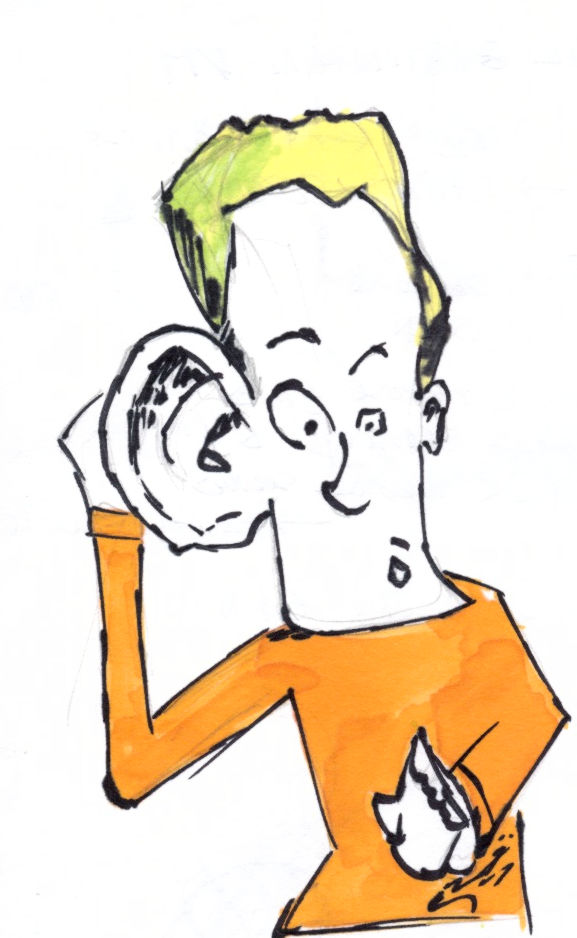
\includegraphics[width=3.125in,height=\textheight]{./images/listen.jpg}

}

\caption{Think of a server as a ``program that listens''. (Source: own
illustration.)}

\end{figure}

\hypertarget{hosting-options}{%
\section{Hosting Options}\label{hosting-options}}

So, where should we go with our project when it outgrows the local
environment of our notebooks? This has actually become a tough question
because of all the reasonable options out there. Technical advances,
almost unparalleled scalability and large profits for the biggest
players made modern infrastructure\index{infrastructure} providers offer
an incredible variety of products to choose from. Obviously, a
description of product offerings in a vastly evolving field is not well
suited for discussions in a book. Hence, \emph{Research Software
Engineering} intends to give an overview to classify the general options
and common business models.

\hypertarget{software-as-a-service}{%
\subsection{Software-as-a-Service}\label{software-as-a-service}}

The simplest solution and fastest time-to-market is almost always to go
for a Software-as-a-Service (SaaS)\index{SaaS} product -- particularly
if you are not experienced in hosting and just want to get started
without thinking about which Linux to use and how to maintain your
server. SaaS products abstract all of that away from the user and focus
on doing one single thing well. The shinyapps.io\footnote{https://shinyapps.io}
platform is a great example of such a service: users can sign up and
deploy their web applications within minutes. The shinyapps.io platform
is a particularly interesting example of a SaaS product because R
developers who come from field-specific backgrounds other than
programming are often not familiar with web development and hosting
websites. Some of these developers, for whom R might be their first
programming language, are suddenly empowered to develop and run online
content thanks to the R Shiny web application framework that uses R to
generate HTML\index{HTML}, CSS and JavaScript\index{JavaScript} based
applications. Still, those applications need to be hosted somewhere.
This is precisely what shinyapps.io does. The service solely hosts web
applications that were created with the Shiny web application framework.
This ease of use is also the biggest limitation of SaaS products. A
website generated with another tool cannot be deployed easily. In
addition, the mere bang-for-buck price is rather high compared to
self-hosting as users pay for a highly, standardized, managed hosting
product. Nevertheless, because of the low volume of most projects, SaaS
is feasible for many projects, especially at a proof of concept stage.

\begin{tcolorbox}[enhanced jigsaw, colback=white, leftrule=.75mm, breakable, colframe=quarto-callout-note-color-frame, bottomrule=.15mm, arc=.35mm, opacityback=0, rightrule=.15mm, toprule=.15mm, left=2mm]
\begin{minipage}[t]{5.5mm}
\textcolor{quarto-callout-note-color}{\faInfo}
\end{minipage}%
\begin{minipage}[t]{\textwidth - 5.5mm}

In case you are interested in getting started with Shiny, take a look at
the Shiny case study in this book. The study explains basic concepts of
Shiny to the user and walks readers through the creation and deployment
of a simple app.

\end{minipage}%
\end{tcolorbox}

SaaS, of course, is neither an R nor a data science idea. Modern
providers offer database\index{database}s, storage calendars, face
recognition and location services, among other things.

\hypertarget{self-hosted}{%
\subsection{Self-Hosted}\label{self-hosted}}

The alternative approach to buying multiple managed services, is to host
your applications by yourself. Since -- this applies to most users at
least -- you do not take your own hardware, connect to your home Wi-Fi
and aim to start your own hosting provider, we need to look at different
degrees of self-hosting. Larger organizations, e.g., universities, often
like to host applications on their own hardware, within their own
network to have full control of their data. Yet, self-hosting exposes
you to issues, such as attacks, that you would not need to worry about
as much in a software as a service setting (as long as you trust the
service).

Self-hosting allows you to host all the applications you want on a
dedicated machine. Self-hosters can configure their server depending on
their access rights. Offerings range from root access that allows users
to do anything to different shades of managed hosting with more
moderated access. Backed by virtual
infrastructure\index{infrastructure}, modern cloud providers offer a
very dynamic form of self-hosting: their clients can use a web GUIs
and/or APIs to add, remove, reboot and shut down nodes. Users can spin
up anything from pre-configured nodes optimized for different use cases
to containerized environments and entire Kubernetes (K8s) clusters in
the cloud. Flexible pricing models allow paying based on usage in a very
dynamic fashion.

\hypertarget{building-blocks}{%
\section{Building Blocks}\label{building-blocks}}

Exactly because of this dynamic described above and the ubiquity of the
cloud, it is good to know about the building blocks of modern IT
infrastructure\index{infrastructure}.

\hypertarget{virtual-machines}{%
\subsection{Virtual Machines}\label{virtual-machines}}

Virtual machines (VMs) remain the go-to building blocks for many
set-ups. Hence, university IT, private sector IT, independent hosting
providers and online giants all offer VMs. Virtual machines allow
running a virtual computer that has its own operating system on some
host machine. Running applications on such a virtual computer feels like
running an application on a standalone computer dedicated to run this
application.

\begin{tcolorbox}[enhanced jigsaw, colback=white, leftrule=.75mm, breakable, colframe=quarto-callout-note-color-frame, bottomrule=.15mm, arc=.35mm, opacityback=0, rightrule=.15mm, toprule=.15mm, left=2mm]
\begin{minipage}[t]{5.5mm}
\textcolor{quarto-callout-note-color}{\faInfo}
\end{minipage}%
\begin{minipage}[t]{\textwidth - 5.5mm}

Oracle's Virtual Box is a great tool to use and try virtual machines
locally. Virtual Box allows to run a Virtual Windows or Linux inside
macOS and vice versa. Running a virtual box locally may not be the most
performant solution, but it allows to have several test environments
without altering one's main environment.

\end{minipage}%
\end{tcolorbox}

\hypertarget{containers-and-images}{%
\subsection{Containers and Images}\label{containers-and-images}}

At the first glance, containers\index{container} look very much like
Virtual Machines\index{Virtual Machines} to the practitioner. The
difference is that every Virtual Machine has its own operating system,
while containers use the host OS to run a container engine on top of the
OS. By doing so, containers can be very lightweight and may take only a
few seconds to spin up, while spinning up Virtual Machines can take up
to a few minutes -- just like booting physical computers. Hence,
Docker\index{Docker} containers are often used as single-purpose
environments: Fire up a container, run a task in that environment, store
the results outside the container and shut down the
container\index{container} again.

Docker\index{Docker} (Why Docker?\footnote{https://www.docker.com/why-docker})
is the most popular containerized solution and quickly became synonymous
to container environments configured in a file. So-called Docker images
are built layer-by-layer based on other less specific Docker images. A
DOCKERFILE\index{DOCKERFILE} is the recipe for a new image. Images are
blueprints for containers\index{container}, an image's running instance.
A Docker runtime environment can build images from
DOCKERFILE\index{DOCKERFILE}s and distribute these images to an image
registry. The platform Docker Hub\footnote{https://dockerhub.com} hosts
a plethora of pre-built Docker images from ready-to-go
database\index{database}s to Python\index{Python} ML environments or
minimal Linux containers to run a simple shell script in a lab-type
environment.

Containers run in a Docker\index{Docker} runtime environment and can
either be used interactively or in batches which execute a single task
in an environment specifically built for this task. One of the reasons
why Docker is attractive to researchers is its open character:
DOCKERFILE\index{DOCKERFILE}s are a good way to share a configuration in
a simple, reproducible file, making it easy to reproduce setups. Less
experienced researchers can benefit from
\href{https://hub.docker.com/}{Docker Hub} which shares images for a
plethora of purposes, from mixed data science setups to
database\index{database} configuration. Side effect free working
environments for all sorts of tasks can especially be appealing in
exotic and/or dependency heavy cases.

Besides simplification of system administration, Docker\index{Docker} is
known for its ability to work in the cloud. All major cloud hosters
offer Docker environments and the ability to deploy Docker containers
that were previously developed and tested locally. You can also use
Docker to tackle \protect\hyperlink{glossary}{throughput problems} using
container orchestration tools like Docker Swarm\footnote{https://docs.docker.com/engine/swarm/swarm-tutorial/}
or K8s (say: Kubernetes)\footnote{https://kubernetes.io/} to run
hundreds of containers (depending on your virtual resources).

\hypertarget{kubernetes}{%
\subsection{Kubernetes}\label{kubernetes}}

Though hosting Kubernetes\index{Kubernetes} (K8s)\index{K8s} is clearly
beyond the scope of basic level DevOps\index{DevOps}, the ubiquity of
the term and technology as well as the touching points and similarities
with the previously introduced concept of containers justify a brief
positioning of Kubernetes. We cannot really see Kubernetes as a building
block like the technologies introduced above. K8s is a complete cluster
with plenty of features to manage the system and its applications.
Kubernetes is designed to run on multiple virtual nodes and distribute
processes running in so-called pods across its nodes.

Because a plain vanilla Kubernetes cluster is not easy to set up and
manage, the tech sector's big three and some of their smaller
alternatives offer their own flavors of cloud-based Kubernetes. The
basic idea of these offerings is to standardize and to take some of the
administrative burden from their clients through pre-configuration and
automation\index{automation} support. Red Hat's Openshift is a different
approach that targets enterprises who want to set up a cluster on their
own infrastructure\index{infrastructure} (on premise).

\hypertarget{applied-containerization-basics}{%
\section{Applied Containerization
Basics}\label{applied-containerization-basics}}

While the above \emph{Building Blocks} section contextualizes the
container\index{containerization} approaches, this section gives a
simple 101 into the basics of containerization\index{containerization},
enabling the readers to take their first steps in the container world.
One of the beautiful things about containers is that, due to their
isolated nature, one can go a long way trying out things as containers
get destroyed and recreated all the time. Also, because
containers\index{container} run in a standardized runtime environment,
locally developed images easily transfer to large remote machines and
clusters.

\hypertarget{dockerfiles}{%
\subsection{DOCKERFILEs}\label{dockerfiles}}

\emph{DOCKERFILE\index{DOCKERFILE}}s\index{Docker} are text file recipes
to create images, i.e., blueprints for containers. One great thing about
container\index{container} images is that they are layered. That is, one
can stack\index{stack} images and benefit from previously created
images. The below example DOCKERFILE\index{DOCKERFILE} uses a standard,
publicly available image from dockerhub.com and adds some custom
packages.

\begin{Shaded}
\begin{Highlighting}[]
\ExtensionTok{FROM}\NormalTok{ rocker/shiny:latest}
\ExtensionTok{RUN}\NormalTok{ apt{-}get update}
\ExtensionTok{RUN}\NormalTok{ apt{-}get install }\AttributeTok{{-}qq} \AttributeTok{{-}y}\NormalTok{ libpq{-}dev}
\ExtensionTok{RUN}\NormalTok{ install2.r ggplot2 shiny shinydashboard  }\DataTypeTok{\textbackslash{}}
\NormalTok{               shinydashboardPlus  }\DataTypeTok{\textbackslash{}}
\NormalTok{               dplyr RPostgres  }
\end{Highlighting}
\end{Shaded}

In this case, we make use of a pre-built image from the rocker project.
The rocker project designs useful images around the R language
ecosystem, builds them on a regular basis and makes them available via
Docker Hub. Here, our image allows running the open source version of
shiny server in a Docker container. We add a Postgres\index{PostgreSQL}
driver at the operating system level before we install several R
packages from CRAN.

\hypertarget{building-and-running-containers}{%
\subsection{Building and Running
Containers}\label{building-and-running-containers}}

There are plenty of ways to run and build containers\index{Docker}.
Online tools either offered as a service or self-hosted can build images
server-side. Yet, the easiest way to get started with containers is to
run and build them locally with Docker Desktop.\\
Even though Docker may not even be the best way to build containers to
some, Docker is by far the most known way and therefore comes with the
largest ecosystem and most community material. Docker Desktop is an
easy-to-use application available on Windows and OSX. With Docker
Desktop, one can execute Docker commands and build images, either in a
GUI or using its CLI. Table~\ref{tbl-dockerbasics} shows a few of the
most basic Docker commands.

\hypertarget{tbl-dockerbasics}{}
\begin{table}
\caption{\label{tbl-dockerbasics}Basic Docker Commands }\tabularnewline

\centering
\begin{tabular}{l>{\raggedright\arraybackslash}p{5.6cm}}
\toprule
Command & Description\\
\midrule
docker run & starts application\\
docker ps & lists containers\\
docker images & lists docker images\\
docker pull & pulls images from registry, e.g., dockerhub.com\\
docker run & runs container based on image\\
\addlinespace
docker kill & kills container\\
docker build <dir-with-docker-file> & builds image based on DOCKERFILE\\
docker exec <command> <container> & executes command inside container\\
\bottomrule
\end{tabular}
\end{table}

To learn what a container looks like, e.g., to find out how the
container was affected by changes to the DOCKERFILE\index{DOCKERFILE},
it can be very illustrative to walk around inside. To do so with a
container created from the above DOCKERFILE\index{DOCKERFILE}, start the
container and execute a bash with the interactive flag \texttt{-it}.

\begin{Shaded}
\begin{Highlighting}[]
\ExtensionTok{docker}\NormalTok{ run }\AttributeTok{{-}d}\NormalTok{ rocker/shiny}
\ExtensionTok{docker}\NormalTok{ exec }\AttributeTok{{-}it}\NormalTok{ rocker/shiny /bin/bash}

\CommentTok{\# alternative you could start R right away}
\CommentTok{\# note that you need to know the location }
\CommentTok{\# of the executable}
\ExtensionTok{docker}\NormalTok{ exec }\AttributeTok{{-}it}\NormalTok{ rocker/shiny /usr/local/bin/R}
\end{Highlighting}
\end{Shaded}

\hypertarget{docker-compose-manage-multiple-containers}{%
\subsection{Docker Compose -- Manage Multiple
Containers}\label{docker-compose-manage-multiple-containers}}

Docker\index{Docker} is a great way to give a new tool a spin without
affecting one's proven environment. So, even if you are a container
beginner, the time when you would like to spin up multiple containers at
once will come quickly. While you can start as many containers as your
local resources allow for, running containers at once does not
necessarily mean those containers are aware of each other, let alone
they could talk to each other.

Modern applications often follow modular architecture patterns, i.e.,
they have a front end, some middle layer such as a REST API and a
database\index{database} backend. A web application may have a
statically generated HTML\index{HTML} front and simply expose
HTML/CSS/JavaScript files and query a REST API. The REST API may use the
express.io framework and is served using a node server which talks to a
Postgres database\index{database} backend. Each of these three parts
could live in its own container. This is where docker could help to
create a development environment locally that essentially mimics the
production setup and therefore facilitates deployment to production.

Docker Compose allows defining how multiple containers play together.
Consider the following example file that creates two containers: a Shiny
web server and a database\index{database} which can be queried by the
Shiny server.

\begin{Shaded}
\begin{Highlighting}[]
\ExtensionTok{services:}
   \ExtensionTok{postgres:}
      \CommentTok{\# a name, e.g.,  db\_container is }
      \CommentTok{\# instrumental to be}
      \CommentTok{\# called as host from the shiny app}
      \ExtensionTok{container\_name:}\NormalTok{ db\_container}
      \ExtensionTok{build:}\NormalTok{ ./postgres}
      \ExtensionTok{restart:}\NormalTok{ always}
      \ExtensionTok{environment:}
         \ExtensionTok{{-}}\NormalTok{ POSTGRES\_USER=postgres}
         \ExtensionTok{{-}}\NormalTok{ POSTGRES\_PASSWORD=postgres}
      \CommentTok{\# This port mapping is only necessary }
      \CommentTok{\# to connect from the host, }
      \CommentTok{\# not to let containers talk to each other. }
      \ExtensionTok{ports:}
         \ExtensionTok{{-}} \StringTok{"5432:5432"}
      \ExtensionTok{volumes:}
         \ExtensionTok{{-}} \StringTok{"./pgdata:/var/lib/postgresql/data"}
   \ExtensionTok{shiny:} 
      \ExtensionTok{container\_name:}\NormalTok{ shiny}
      \ExtensionTok{depends\_on:} 
         \ExtensionTok{{-}}\NormalTok{ postgres}
      \ExtensionTok{build:}\NormalTok{ ./shiny}
      \ExtensionTok{volumes:}
         \ExtensionTok{{-}} \StringTok{"./shiny{-}logs:/var/log/shiny{-}server"}
         \ExtensionTok{{-}} \StringTok{"./shiny{-}home:/srv/shiny{-}server"}
      \ExtensionTok{ports:}
         \ExtensionTok{{-}} \StringTok{"3838:3838"}
\end{Highlighting}
\end{Shaded}

Note how images are built from local directories \texttt{postgres} and
\texttt{shiny} that contain DOCKERFILE\index{DOCKERFILE}s. It is also
possible to pull images directly from a registry. To run such a system
of multiple containers, simply use

\begin{Shaded}
\begin{Highlighting}[]
\ExtensionTok{docker}\NormalTok{ compose up }\AttributeTok{{-}{-}force{-}recreate}
\end{Highlighting}
\end{Shaded}

\begin{tcolorbox}[enhanced jigsaw, colback=white, leftrule=.75mm, breakable, colframe=quarto-callout-note-color-frame, bottomrule=.15mm, arc=.35mm, opacityback=0, rightrule=.15mm, toprule=.15mm, left=2mm]
\begin{minipage}[t]{5.5mm}
\textcolor{quarto-callout-note-color}{\faInfo}
\end{minipage}%
\begin{minipage}[t]{\textwidth - 5.5mm}

Note that \emph{docker-compose} does not replace an orchestrator and
cannot provide cluster functionality like Docker Swarm or even
Kubernetes.

\end{minipage}%
\end{tcolorbox}

\hypertarget{a-little-docker-debugging-tip}{%
\subsection{A Little Docker Debugging
Tip}\label{a-little-docker-debugging-tip}}

Sometimes containers keep crashing right after they start\index{Docker}.
This makes debugging a bit harder because we cannot simply use the
\texttt{-it} flag to get inside and stroll around to find the issue. In
such a case, even if you briefly log in, your container will shut down
before you can even reach the location in question inside your
container. Of course, there are log files

\begin{Shaded}
\begin{Highlighting}[]
\ExtensionTok{docker}\NormalTok{ logs }\OperatorTok{\textless{}}\NormalTok{container{-}name}\OperatorTok{\textgreater{}}
\end{Highlighting}
\end{Shaded}

Maybe though these logs are not verbose enough, or some permission issue
may not be fully covered. Hence, adding `command: ``sleep infinity'' to
your compose file prevents the service/container in question from
running into the problem and crashing immediately.

\bookmarksetup{startatroot}

\hypertarget{sec-auto}{%
\chapter{Automation}\label{sec-auto}}

\begin{quote}
Make repetitive work fun again!
\end{quote}

One aspect that makes a programming approach to data science and
analytics appealing is \emph{automation\index{automation}}. Data
ingestion, dissemination, reporting or even analysis itself can be
repetitive. Particularly shorter update cycles of one's data ask for a
way to make yet another iteration pain-free. The following sections look
at different forms of automation\index{automation} such as continuous
integration and deployment, different forms of workflow
automation\index{automation} as well as
infrastructure\index{infrastructure} as code.

\hypertarget{continuous-integrationcontinuous-deployment}{%
\section{Continuous Integration/Continuous
Deployment}\label{continuous-integrationcontinuous-deployment}}

Because of its origin in build, test and check
automation\index{automation}, Continuous Integration/Continuous
Deployment (CI/CD\index{CI/CD})\footnote{See also:
  https://www.atlassian.com/continuous-delivery/principles/continuous-integration-vs-delivery-vs-deployment}
may not be the first thing that comes into mind when one approaches
programming through the analytics route. Yet, thorough testing and
automated builds have not only become well-established parts of the data
science workflow, CI/CD\index{CI/CD} tools can also help to automate
tasks beyond testing and packaging your next release.

Modern \index{version control} software providers are an easy way to add
the tool chain that is often fuzzily called CI/CD\index{CI/CD}. While CI
stands for \emph{continuous integration} and simply refers to a workflow
in which the team tries to release new features to production as
continuously as possible, CD stands for either \emph{continuous
delivery} or \emph{continuous deployment}.

Thanks to infrastructure\index{infrastructure} as code and
containerization\index{containerization}, automation\index{automation}
of development and deployment workflows become much easier also because
local development can run in an environment very close to the production
setup. Git hosting powerhouses GitHub\index{GitHub} and
GitLab\index{GitHub} run their flavors of CI/CD\index{CI/CD} tools,
making the approach well documented and readily available by default to
a wide array of users: GitHub Actions\footnote{https://docs.github.com/en/actions}
and GitLab CI\footnote{https://docs.gitlab.com/ee/ci/}. In addition,
services like CircleCI\footnote{https://circleci.com/} offer this
toolchain independently of hosting git repositories.

Users of the above platforms can upload a simple text file that follows
a name convention and structure to trigger a step-based tool-chain based
on an event. An example of an event may be a push to a repository's main
branch. A common example would be to run tests and/or build a package
and upon success deploy the newly created package to some server -- all
triggered by a simple push to master. One particularly cool thing is,
that there are multiple services which allow running the testing on
their servers using container technologies. This leads to a great
variety of setups for testing. That way, software can easily be tested
on different operating systems/environments.

Here is a simple sketch of a \emph{.gitlab-ci.yml} configuration that
builds and tests on pushes to all branches and deploys a package after a
push to the main branch and successful build and test steps:

\begin{verbatim}
stages:
- buildncheck
- deploy_pack

test:
image:
name: some.docker.registry.com/some-image:0.2.0
entrypoint:
- ""
stage: buildncheck
artifacts:
untracked: true
script:
# we don't need it and it causes a hidden file NOTE
- rm .gitlab-ci.yml 
- install2.r --repos custom.mini.cran.ch .
- R CMD build . --no-build-vignettes --no-manual
- R CMD check --no-manual *.tar.gz

deploy_pack:
only: 
- main
stage: deploy_pack
image:
name: byrnedo/alpine-curl
entrypoint: [""]
dependencies:
- 'test'
script:
- do some more steps to login and deploy to server ...
\end{verbatim}

For more in depth examples of the above, Jim Hester's talk on
GitHub\index{GitHub} Actions for R\footnote{https://www.jimhester.com/talk/2020-rsc-github-actions/}
is an excellent starting point. CI/CD\index{CI/CD} tool chains are
useful for a plethora of actions beyond mere building, testing and
deployment of software. The publication chapter covers another common
use case: rendering and deployment of static websites. That is, websites
that are updated by re-rendering their content at build time, creating
static files (artifacts) that are uploaded to web host. Outlets like the
GitHub Actions Marketplace, the r-lib collections for R specific actions
and the plethora of readily available actions are a great showcase of
the broad use of CI/CD\index{CI/CD} applications.

\hypertarget{cron-jobs}{%
\section{\texorpdfstring{Cron
Jobs\index{cron job}}{Cron Jobs}}\label{cron-jobs}}

Cron syntax is very common in the Unix world and is also useful in the
context of the CI/CD\index{CI/CD} tools explained above. Instead of
\emph{on dispatch} or \emph{event based} triggers, CI/CD\index{CI/CD}
processes can also be triggered based on time.

Named after the Unix job scheduler \emph{cron}, a cron job is a task
that runs periodically at fixed times. Pre-installed in most Linux
server setups, data analysts often use cronjobs\index{cron job} to
regularly run batch jobs on remote servers. Cron jobs use a funny syntax
to determine when jobs run.

\begin{Shaded}
\begin{Highlighting}[]
\CommentTok{\#min hour day month weekday}
\ExtensionTok{15}\NormalTok{ 5,11 }\PreprocessorTok{*} \PreprocessorTok{*}\NormalTok{ 1 Rscript run\_me.R}
\end{Highlighting}
\end{Shaded}

The first position denotes the minute mark at which the job runs -- in
our case 15 minutes after the new hour started. The second mark denotes
hours during the day -- in our case the 5th and 11th hour. The asterisk
* is a wildcard expression for running the job on every day of the month
and in every month throughout the year. The last position denotes the
weekday, in this example we run our job solely on Mondays.

More advanced expressions can also handle running a job at much shorter
intervals, e.g., every 5 minutes.

\begin{Shaded}
\begin{Highlighting}[]
\ExtensionTok{*/5} \PreprocessorTok{*} \PreprocessorTok{*} \PreprocessorTok{*} \PreprocessorTok{*}\NormalTok{ Rscript check\_status.R}
\end{Highlighting}
\end{Shaded}

To learn and play with more expressions, check crontab guru\footnote{https://crontab.guru/}.
If you have more sophisticated use cases, like overseeing a larger
number of jobs or execution on different nodes, consider using Apache
Airflow\index{Apache Airflow}\footnote{https://airflow.apache.org/} as a
workflow scheduler.

\hypertarget{workflow-scheduling-apache-airflow-dags}{%
\section{\texorpdfstring{Workflow Scheduling: Apache
Airflow\index{Apache Airflow}
DAGs}{Workflow Scheduling: Apache Airflow DAGs}}\label{workflow-scheduling-apache-airflow-dags}}

Though much less common than the above tools,
\href{https://airflow.apache.org/}{Apache Airflow} has earned a mention
because of its ability to help researchers keep an overview of regularly
running processes. Examples of such processes could be daily or monthly
data sourcing or timely publication of a regularly published indicator.
I often referred to Airflow as ``cronjobs\footnote{https://en.wikipedia.org/wiki/Cron}
on steroids.'' Airflow ships with a dashboard to keep track of many
timed processes, plus a ton of other logs and reporting features, which
are worth a lot when maintaining reoccurring processes. Airflow has its
own \emph{Airflow Summit} conference, a solid community and Docker
compose setup to get you started quickly. The setup consists of a
container image for the web frontend and another image for the
PostgreSQL\index{PostgreSQL} backend. The fact that there is also a
\emph{Managed Workflow for Apache Airflow\index{Apache Airflow}}
offering in the Amazon cloud at the time of writing shows the broad
acceptance of the tool. Airflow also runs on Kubernetes in case you are
interested in hosting Airflow in a more robust production setup.

So, what does Airflow look like in practice? Airflow uses the
Python\index{Python} language to define directed acyclic graphs (DAGs).
Essentially, a DAG pictures a process that has -- unlike a cycle -- a
clear start and ending. DAGs can be one-dimensional and fully
sequential, but they can also run tasks in parallel.

\begin{Shaded}
\begin{Highlighting}[]
\ImportTok{from}\NormalTok{ datetime }\ImportTok{import}\NormalTok{ datetime, timedelta}
\ImportTok{from}\NormalTok{ airflow }\ImportTok{import}\NormalTok{ DAG}
\CommentTok{\# Operators; we need this to operate!}
\ImportTok{import}\NormalTok{ BashOperator}
\ControlFlowTok{with}\NormalTok{ DAG(}
\NormalTok{    default\_args}\OperatorTok{=}\NormalTok{\{}
        \StringTok{"depends\_on\_past"}\NormalTok{: }\VariableTok{False}\NormalTok{,}
        \StringTok{"email"}\NormalTok{: [}\StringTok{"airflow{-}admin@your{-}site.com"}\NormalTok{],}
        \StringTok{"email\_on\_failure"}\NormalTok{: }\VariableTok{False}\NormalTok{,}
        \StringTok{"email\_on\_retry"}\NormalTok{: }\VariableTok{False}\NormalTok{,}
        \StringTok{"retries"}\NormalTok{: }\DecValTok{1}\NormalTok{,}
        \StringTok{"retry\_delay"}\NormalTok{: timedelta(minutes}\OperatorTok{=}\DecValTok{5}\NormalTok{)}
\NormalTok{    \},}
\NormalTok{    description}\OperatorTok{=}\StringTok{"Bash Operator"}
\NormalTok{    schedule}\OperatorTok{=}\StringTok{\textquotesingle{}5 11 * * *\textquotesingle{}}\NormalTok{,}
\NormalTok{    start\_date}\OperatorTok{=}\NormalTok{datetime(}\DecValTok{2023}\NormalTok{, }\DecValTok{1}\NormalTok{, }\DecValTok{1}\NormalTok{),}
\NormalTok{    catchup}\OperatorTok{=}\VariableTok{False}\NormalTok{,}
\NormalTok{    tags}\OperatorTok{=}\NormalTok{[}\StringTok{"example"}\NormalTok{],}
\NormalTok{) }\ImportTok{as}\NormalTok{ dag:}
    \CommentTok{\# t1, t2 and t3 are examples of tasks}
    \CommentTok{\# created by instantiating operators}
\NormalTok{    t1 }\OperatorTok{=}\NormalTok{ BashOperator(}
\NormalTok{        task\_id}\OperatorTok{=}\StringTok{"print\_date"}\NormalTok{,}
\NormalTok{        bash\_command}\OperatorTok{=}\StringTok{"date \textgreater{} date.txt"}\NormalTok{,}
\NormalTok{    )}

\NormalTok{    t2 }\OperatorTok{=}\NormalTok{ BashOperator(}
\NormalTok{        task\_id}\OperatorTok{=}\StringTok{"sleep"}\NormalTok{,}
\NormalTok{        depends\_on\_past}\OperatorTok{=}\VariableTok{False}\NormalTok{,}
\NormalTok{        bash\_command}\OperatorTok{=}\StringTok{"sleep 5"}\NormalTok{,}
\NormalTok{        retries}\OperatorTok{=}\DecValTok{3}\NormalTok{,}
\NormalTok{    )}
    
\NormalTok{    t3 }\OperatorTok{=}\NormalTok{ BashOperator(}
\NormalTok{        task\_id}\OperatorTok{=}\StringTok{"2 dates"}\NormalTok{,}
\NormalTok{        depends\_on\_past}\OperatorTok{=}\VariableTok{False}\NormalTok{,}
\NormalTok{        bash\_command}\OperatorTok{=}\StringTok{"cat date.txt \& date"}\NormalTok{,}
\NormalTok{    )}

\NormalTok{    t1 }\OperatorTok{\textgreater{}\textgreater{}}\NormalTok{ t2 }\OperatorTok{\textgreater{}\textgreater{}}\NormalTok{ t3}
\end{Highlighting}
\end{Shaded}

The above code shows an example of a simple DAG that combines three
strictly sequential tasks. Task \emph{t1} depends on tasks \emph{t2} and
\emph{t3}. In this simple example, all tasks use the Airflow
\emph{BashOperator} to execute Bash commands, but Airflow provides
plenty of other operators from its \emph{PythonOperator}\index{Python},
to \emph{Docker} or \emph{Kubernetes} operators.\\
Such operators also allow executing tasks on remote machine or clusters,
not solely the machine or container that serves Airflow itself.

\hypertarget{make-like-workflows}{%
\section{\texorpdfstring{Make-Like
Workflows\index{Makefile}}{Make-Like Workflows}}\label{make-like-workflows}}

\emph{Makefiles} and the \emph{make} software that made them popular are
the classic of build automation\index{automation}. Best known for its
support in the compilation of C programs, Makefiles became popular
across programming languages thanks to their straightforward concept and
readable approach. A Makefile contains a \emph{target}, an optional
prerequisite, and a recipe to get there.

\begin{Shaded}
\begin{Highlighting}[]
\ExtensionTok{target:}\NormalTok{ prerequisite}
    \ExtensionTok{recipe}
\end{Highlighting}
\end{Shaded}

Like this:

\begin{Shaded}
\begin{Highlighting}[]
\ExtensionTok{say\_yo:}\NormalTok{ store\_yo}
    \FunctionTok{cat}\NormalTok{ echo.txt}

\ExtensionTok{store\_yo:} 
    \BuiltInTok{echo} \StringTok{"yo!"} \OperatorTok{\textgreater{}}\NormalTok{ echo.txt}
\end{Highlighting}
\end{Shaded}

This will simply print

\begin{Shaded}
\begin{Highlighting}[]
\BuiltInTok{echo} \StringTok{"yo!"} \OperatorTok{\textgreater{}}\NormalTok{ echo.txt}
\FunctionTok{cat}\NormalTok{ echo.txt}
\ExtensionTok{yo!}
\end{Highlighting}
\end{Shaded}

in your terminal. Very much like Apache Airflow\index{Apache Airflow}
and its DAGs which were introduced above, Makefiles allow declaring and
managing dependencies. The ability of make and make-like approaches such
as the \{targets\} R package (Landau 2021) goes well beyond the simple
sequential definitions like the basic example above. Parallel execution
of independent tasks, cherry-picking execution of single tasks from a
larger workflow, variables and caching are highly useful when runtime
increases. Consider, a multistep workflow, parts of which are running
for quite a while but hardly change while other swift parts change all
the time, and it becomes obvious how a simple CLI-based workflow
helps.\\
Modern implementation like the target R package ship with network
visualizations of the execution path and its dependencies. The
walkthrough provided in R OpenSci's book\footnote{https://books.ropensci.org/targets/walkthrough.html}
on target is a great summary available as text, code example and video.

\hypertarget{infrastructure-as-code}{%
\section{\texorpdfstring{infrastructure\index{infrastructure} as
Code}{infrastructure as Code}}\label{infrastructure-as-code}}

In recent years, declarative approaches helped to make task
automation\index{automation} more inclusive and appealing to a wider
audience. Not only a workflow itself, but also the environment a
workflow should live and run in is often defined in declarative fashion.
This development does not only make maintenance easier, it also helps to
make a setting reproducible and shareable.

Do not think infrastructure\index{infrastructure} as code is only
relevant for system admins or other infrastructure\index{infrastructure}
professionals who make use of it every day. The ability to reproduce and
tweak infrastructure\index{infrastructure} at essentially no costs
enables other forms of automation\index{automation} such as
CI/CD\index{CI/CD}. Just like a flat rate with your mobile carrier will
lead to more calls.

infrastructure\index{infrastructure} as code approaches do not only
describe infrastructure\index{infrastructure} in declarative and
reproducible fashion as stated above;
infrastructure\index{infrastructure}-as-code can also be seen as a way
to automate setting up the environment you work with. The
infrastructure\index{infrastructure} section explains in greater detail
how such definitions look like and containers are building blocks of
modern infrastructure\index{infrastructure} defined in code.

automation\index{automation} is more complex for cluster setups because
among other things, applications need to be robust against pods getting
shut down on one node and spawned on another node allowing to host
applications in \emph{high availability} mode. On Kubernetes clusters,
Helm\footnote{https://helm.sh/}, Kubernetes' package manager, is part of
the solution to tackle this added complexity. Helm is, as the Helm
website defines ``the best way to find share and use software built for
Kubernetes''. Terraform\footnote{https://www.terraform.io/} can manage
Kubernetes clusters on clouds like Amazon's AWS, Google's GPC,
Microsoft's Azure and many other cloud systems using declarative
configuration files. Again, a console-based client interface is used to
apply a declarative configuration plan to a particular cloud.

\bookmarksetup{startatroot}

\hypertarget{community}{%
\chapter{Community}\label{community}}

Besides the free-of-license-costs argument, the open source community
may be the most popular argument in favor of open source software. And
the added value of the community is almost certainly much more valuable
than a few green bucks saved on licenses. The support of some of the
best communities is so good it may very well outperform an internal IT
department specialized elsewhere. Still, developer communities do have
their idiosyncrasies. This section intends to help overcome entry
barriers and encourage the reader to connect to the developer
communities -- even if one is not a regular active contributor.

\begin{figure}

{\centering 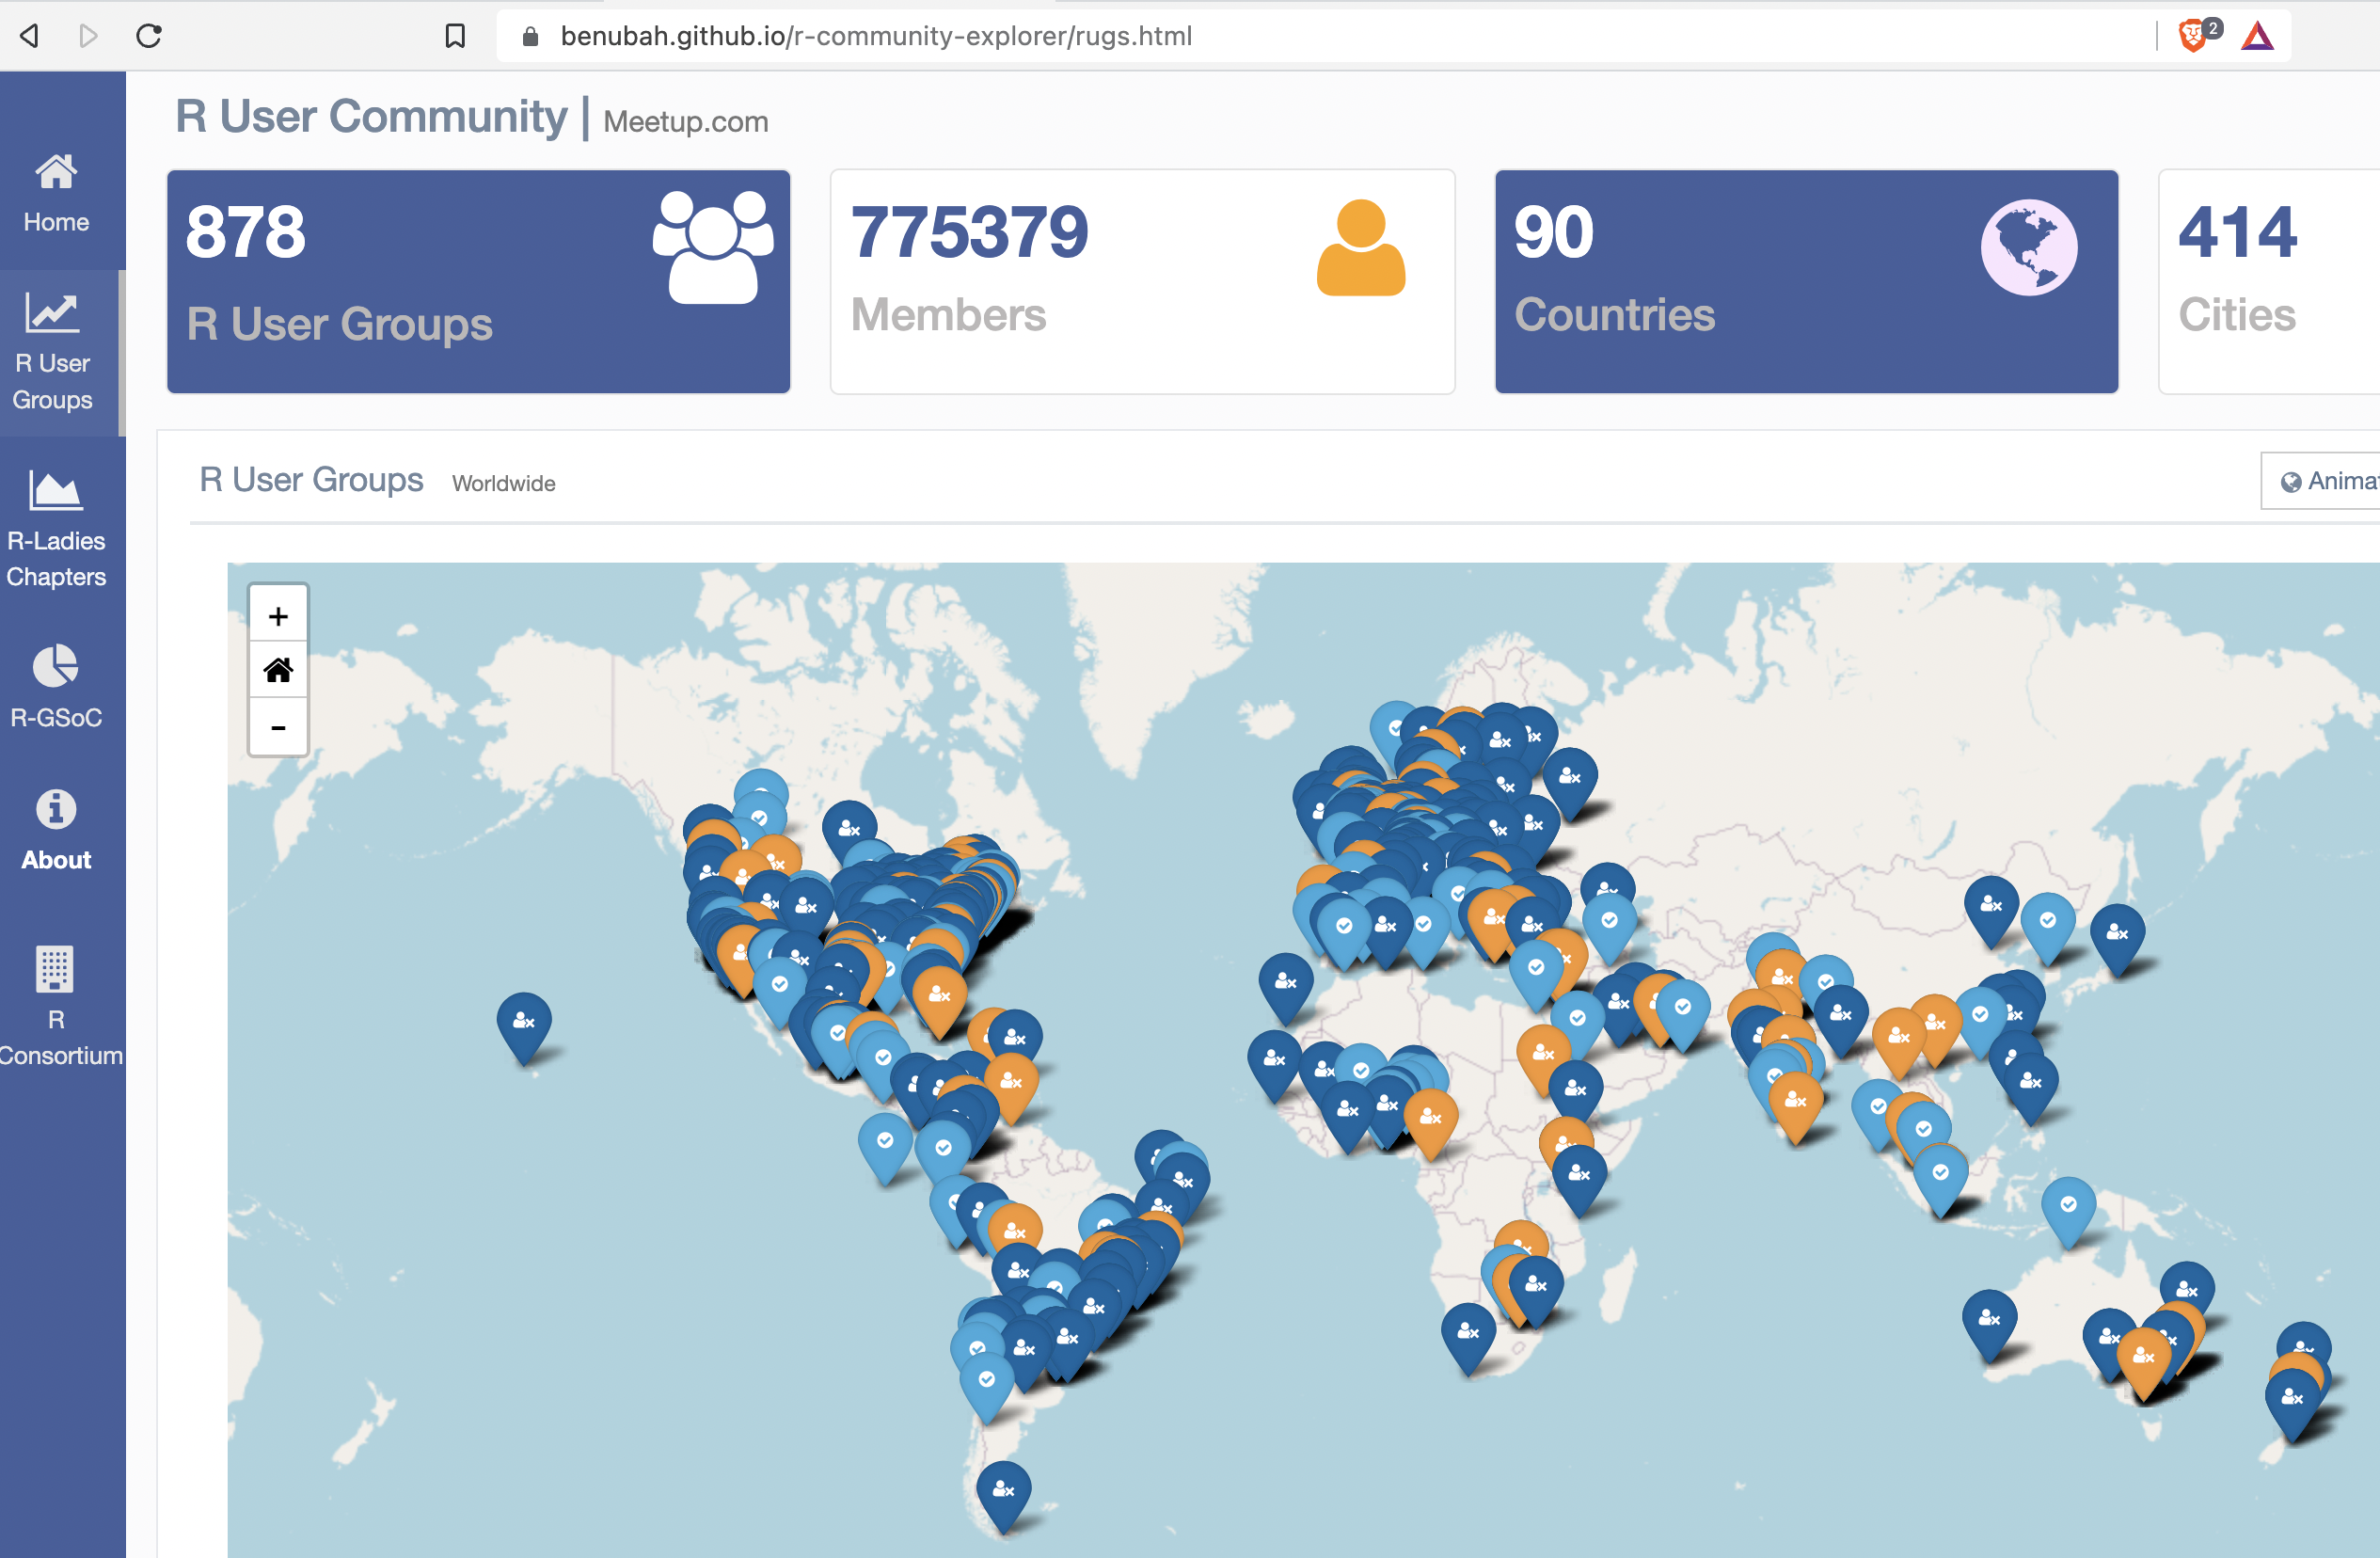
\includegraphics{./images/community_explorer.png}

}

\caption{R Community Explorer by Ben Ubah. (Source:
benubah.github.io/r-community-explorer/rugs.html)}

\end{figure}

The above figure shows a screenshot of an interactive community explorer
tool for the R community. Users can explore user groups and such as R
user groups or RLadies chapters around the world. At the time of
writing, the tool counted more than 775,000 members of R user groups
worldwide and more than 100,000 members of RLadies. The explorer tool
and its numbers should not only show you the size of the community, but
also help to connect to what has become a very global community.

Apart from user groups of programming languages, the Society of Research
Software
Engineering\footnote{https://society-rse.org/}\index{Society of Research Software Engineering}
is a good way to connect. In addition to the UK-based origin, the
society has expanded to other countries and has derivatives in, e.g.,
the United States\footnote{https://us-rse.org/} or Germany\footnote{https://de-rse.org/de/index.html}.
The main idea of research software engineering societies is to work on a
role of software engineering in academia that accounts for the
importance and impact of software on modern research. This goes from
education in programming to lobbying for acknowledgement of software
engineering in academic resumés.

The below sections introduce different channels to connect and interact
with the community. Of course, we do not have to use all of these tools
and be active in all of these communities, but rather pick some that
suit our way of communication.

\hypertarget{stay-up-to-date-in-a-vastly-evolving-field-social-media}{%
\section{Stay Up-to-Date in a Vastly Evolving Field -- Social
Media}\label{stay-up-to-date-in-a-vastly-evolving-field-social-media}}

I hate to admit it because I am not a big fan of social media, but it
has definitely become an important channel for professional use also to
me. Social media is a great way to get my regular dose of what's new in
tech. The popularity of platforms varies locally but also evolves pretty
dynamically over time. \emph{X}, back when it was called Twitter, had
been the platform of choice for many engineers around data science for
almost a decade, before large chunks turned their back on the chirping
platform. I am still there\footnote{https://x.com/whatsgoodio}, but I
may have to find a new tool to get feedback and bookmark good reads. No
matter the platform, make sure not to get caught in politics, memes or
cat pictures if you use it professionally. Because once you strictly
limit your time and avoid going down too many rabbit holes, you will get
a programming tip here, a nice shortcut there and, more importantly, get
a sense of trends and dynamics.

Start with a few accounts to follow, adapt them regularly and use lists
in case you need to organize your input a bit more. For \emph{X}, Tweet
Deck is a good standard option for a more advanced use of the platform.
If you plan to build some following of your own, learn how to schedule
posts and put some thought into the timing of your outlet, regarding
time zone and audience.

\hypertarget{knowledge-sharing-platforms}{%
\section{Knowledge-Sharing
Platforms}\label{knowledge-sharing-platforms}}

The most popular knowledge-sharing platform for programmers,
stack\index{stack}overflow.com, has made itself a name for being the
first hit in your favorite search engine to any questions or error
messages remotely related to source code. The platform has accumulated
millions of questions and answers to programming questions across
languages. Through a mix of quality content, a community rating system
and a healthy mix of gamification, the platform managed to become a
mainstay of the programming community. The platform's crowd-based rating
system does not only assess the quality of questions and answers, a
solid stack\index{stack} Overflow score and reach have also become a
notch on programmers' resumés.

\hypertarget{look-out-for-local-community-group}{%
\section{Look Out for Local Community
Group}\label{look-out-for-local-community-group}}

Speaking of job market opportunities, look out for a local R,
Python\index{Python}\} or data science user group. Local user groups
around programming languages do not only host interesting talks or other
formats, they often provide an opportunity to network or even have
dedicated time to advertise open positions. Besides the community
explorer mentioned in the introduction of this chapter, the
meetup\footnote{https://www.meetup.com/} platform that has become
synonymous with special interest groups coming together locally, is a
good place to start your research.

\hypertarget{attend-conferences---online-can-be-a-viable-option}{%
\section{Attend Conferences - Online Can Be a Viable
Option!}\label{attend-conferences---online-can-be-a-viable-option}}

In similar fashion, conferences are a good channel to stay connected and
up-to-date. A conference like PiConf\footnote{https://piconf.net/},
Posit Conf or useR!\footnote{https://x.com/\_useRconf} is basically a
bulk meetup: potentially hundreds of talks, thousands of potential
contacts, and quite a bit of time to digest a large conference. In
recent years, conferences often provide an option to attend online.
While, to some, most of the fun and networking will be missing online,
the ability to attend online can also be a great chance for a conference
and its attendance. Online conferences have the chance to be a lot more
inclusive than their in-person counterparts. Even costs aside, i.e.,
covered by scholarships, many cannot afford the time to leave their jobs
and families to travel internationally for an entire week. Online
conferences also give people a chance to attend who may not be involved
enough to attend a software development conference for an entire week,
but who want to catch a glimpse and evaluate. In any case, the entry
hurdle is lower than ever. These paragraphs are meant to convince you to
take your time, to prepare, attend and debrief a major open source
software conference -- online or in-person.

\hypertarget{join-a-chat-space}{%
\section{Join a Chat Space}\label{join-a-chat-space}}

Community chat spaces run by conference organizers, local user groups or
societies are another way to stay connected to the community. More
dynamic than message boards and forums, chats allow for both
asynchronous and live communication. Usually chat spaces are more
domain- or even topic-specific than local meetups or social media.
Popular software to participate or even run one's own community is
Slack\footnote{https://slack.com}, Discord\footnote{https://discord.com/},
Mattermost\footnote{https://mattermost.com/} or Matrix\footnote{https://matrix.org/}.
Slack is available as a service run by a company of the same name. Slack
users can start new workspaces for free for hundreds of members, but
will have to pay when they want to keep their communities messages
beyond the last 10,000 messages. Just like Slack, \emph{Discord} works
in our web browsers or as a standalone Desktop or mobile client. Popular
among gamers, Discord does not quite have the business attire of Slack,
but it certainly has its fans. Mattermost is an open source alternative
to the former two. It is also available as a service, but is rather
known as a package to self-host one's independent chat space. Matrix has
a different approach, labelling itself \emph{an open network for secure,
decentralized communication}. Reminiscent of the Internet Relay Chat
(IRC)\footnote{https://en.wikipedia.org/wiki/Internet\_Relay\_Chat} of
the old days, Matrix is server software and network of the same name.
Just like IRC, Matrix is not bound to a single client and therefore
appears modular to the end users allowing to choose between different
clients such as Element\footnote{https://element.io/} to connect to
established and self-hosted networks alike.

\bookmarksetup{startatroot}

\hypertarget{publishing-and-reporting-1}{%
\chapter{Publishing and Reporting}\label{publishing-and-reporting-1}}

Business analysts are used to reporting to management and/or clients
regularly. Modern academic research has a similar need for regular
updates: Data might get revised or otherwise updated, journals,
reviewers and readers will ask for reproducible research. Dissemination
of datasets and results in visually appealing as well as
machine-readable fashion are important academic, private and public data
workers alike.

Because of frequent updates and reproducibility, manually composed
outlets become less sustainable. Luckily, Markdown-based reporting
offers great solutions for presentations, websites, reports, blogs,
office documents or even printed output. Document converters can turn
Markdown into HTML/CSS/JavaScript \index{JavaScript} output for flexible
use in a standard web browser. Likewise, Markdown renders to PDF or even
Microsoft Word.

Approaches\index{Quarto} such as Quarto\footnote{https://Quarto.org} (J.
J. Allaire et al. 2022), RMarkdown\index{RMarkdown} (J. Allaire et al.
2022) or Jupyter Notebooks\index{Jupyter} (Beg et al. 2021) mix plain
text with dynamically rendered code chunks that create tables or figures
and embed these into the document in the right size and spot. Such a
setup is the basis to fully automate the way from analysis to report no
matter whether the outlet is printed, a Word document, a presentation,
blog or website.

\hypertarget{getting-started-with-a-simple-report}{%
\section{Getting Started with a Simple
Report}\label{getting-started-with-a-simple-report}}

The simplest form of such a Markdown-based output, is a simple
HTML\index{HTML} report.\\
To those of us without a web development past or present, HTML may
rather sound daunting than simple. But hear me out: HTML\index{HTML} is
(a) a lot more useful and flexible than newcomers might think and (b)
simple indeed: HTML is text, does not need LaTeX to be rendered from
Markdown like PDF, and can be displayed by web browsers on a plethora of
devices. Plus, based on HTML, you can create (fancy) presentations,
websites or simple reports. With the self-contained option, you can even
embed included files such as images into one single HTML document using
byte encoding. That way, you can easily share a report that can be
viewed on any device with a web browser across different operating
systems and setups.\\
To see a Markdown process in action, consider the following basic
example of Markdown syntax:

\begin{Shaded}
\begin{Highlighting}[]
\NormalTok{\#| output: asis}


\FunctionTok{\#\# This is a level two header \{.unlisted\}}

\NormalTok{This is plain text *this is italic*}
\NormalTok{and **this is bold**}

\FunctionTok{\#\#\# This is a level three header \{.unlisted\}}

\NormalTok{more text}
\end{Highlighting}
\end{Shaded}

When rendered, the above Markdown turns into the below output, stored in
HTML and CSS files.

\hypertarget{this-is-a-level-two-header}{%
\section{This is a level two header}\label{this-is-a-level-two-header}}

This is plain text \emph{this is italic} and \textbf{this is bold}

\hypertarget{this-is-a-level-three-header}{%
\subsection{This is a level three
header}\label{this-is-a-level-three-header}}

more text

\hypertarget{static-website-generators}{%
\section{\texorpdfstring{Static Website
Generators\index{Static Website Generator}}{Static Website Generators}}\label{static-website-generators}}

Once we understood how the output files are created, let's take a more
in-depth look at how a report goes online in fully automated fashion
from computation to a website. In a nutshell, static website generators
turn Markdown code into a combination of HTML\index{HTML}, CSS and
JavaScript, so a web browser can display the result. The Go
based\index{Hugo} Hugo\footnote{https://gohugo.io/} or the
classic\index{Jekyll} Jekyll\footnote{https://jekyllrb.com/} are popular
static website generator approaches to run a website or blog.

Approaches such as the \{distill\} R package (Dervieux et al. 2022) or
Quarto\index{Quarto}, the new kid on the block, add a data science and
analytics flavor to the static website generator approach: Those
implementations allow running analytics' code at render time.
Quarto\index{Quarto} documents, for example, are text files that contain
Markdown text and possibly code chunks in the same documents. When
rendered, the analytics code runs first, potentially creating output
such as tables or figures. If necessary, this output is stored in
separate files and smoothly integrated into the main document that is
about to be rendered afterward.

Rendered output often consists of multiple files such as HTML documents,
CSS style information, JavaScript code or images. Because this may be
fine for websites but inconvenient for presentations or the exchange of
reports, analytics-minded renderers such as Quarto\index{Quarto} offer a
\textbf{self-contained} option. When enabled, Quarto\index{Quarto}
renders a single self-contained, encoded HTML file that contains
everything from JavaScript\index{JavaScript} to images.

\hypertarget{hosting-static-websites}{%
\section{Hosting Static Websites}\label{hosting-static-websites}}

Because the requirements of a static website are minimal, we can
essentially use the simplest website host possible to host our static
site. Unlike with content management system approaches such as
WordPress, static websites do not need server side scripting languages
or database\index{database}s. This simplicity allows hosting static
websites on a plethora of cheap hosters, including many free plans.

\hypertarget{github-pages}{%
\subsection{GitHub Pages}\label{github-pages}}

One excellent and simple solution to host blogs, personal websites,
online documentation or presentations is to use the offerings of major
git providers such as GitHub's GitHub\index{GitHub} Pages\footnote{https://pages.github.com/}.
Though originally meant to be used with themes provided by GitHub and
Markdown rendered by Jekyll on GitHub's servers, GitHub Pages became the
home of an abundance of static sites rendered by a wide array of static
website generators.

All you need is a repository on GitHub to host the static files. You can
activate GitHub Pages for your repository and choose whether you rather
want the rendered files to be on a separate branch named \emph{gh-pages}
or in a subfolder of your root directory (mostly docs). Personally, I
favor using a separate \emph{gh-pages} branch because git would track
every single change made to the automatically rendered content, leading
to a messy git history.

By convention, the corresponding static website of a git repository is
exposed at
\texttt{\textless{}username\textgreater{}.github.io/\textless{}repository-name\textgreater{}}.
For GitHub organizations which are popular to group repositories, the
exposed URL would be
\texttt{\textless{}orgname\textgreater{}.github.io/\textless{}repository-name\textgreater{}}.

\begin{tcolorbox}[enhanced jigsaw, left=2mm, arc=.35mm, colbacktitle=quarto-callout-note-color!10!white, breakable, colframe=quarto-callout-note-color-frame, bottomrule=.15mm, bottomtitle=1mm, colback=white, leftrule=.75mm, coltitle=black, toptitle=1mm, titlerule=0mm, title=\textcolor{quarto-callout-note-color}{\faInfo}\hspace{0.5em}{Note}, opacityback=0, rightrule=.15mm, toprule=.15mm, opacitybacktitle=0.6]

Note that the online version of the book you are currently reading is
hosted in very similar fashion: \texttt{rse-book.github.io}

\end{tcolorbox}

\hypertarget{github-actions}{%
\subsection{\texorpdfstring{GitHub\index{GitHub}
Actions}{GitHub Actions}}\label{github-actions}}

Hosting a website on a modern git platform comes with an intriguing
option: the use of continuous integration tools, as discussed in
Chapter~\ref{sec-auto} on automation\index{automation}.
CI/CD\index{CI/CD} is capable of not only rendering Markdown, but can
even run computations and virtually any prerequisite step thanks to the
underlying docker\index{Docker} technology. CI/CD\index{CI/CD} certainly
introduces a setup hurdle, but it allows integrating users who do not
have the necessary stack\index{stack} installed to execute the render
process locally.

\hypertarget{netlify}{%
\subsection{Netlify}\label{netlify}}

The Netlify\footnote{https://netlify.app/} platform does not host git
repositories like GitHub\index{GitHub} or Bitbucket, but it rather
focuses on the \emph{build} part. Netlify supports the user in setting
up the build process and offers a few add-ons such as Netlify forms to
allow for website features that can process user interaction such as
online forms. Also, unlike git platforms, Netlify integrates domain
purchase into its own platform. Note that Netlify and git are
complementary, not mutually exclusive approaches. Platforms like Netlify
and GitHub\index{GitHub} use application programming interfaces (APIs)
to communicate with each other, allowing to trigger Netlify builds based
on changes to a GitHub repositories.

Basic GitHub\index{GitHub} Pages setups are good enough for online
documentation of most software or other sites that simply display static
content. Netlify cannot only improve convenience when using advanced
features, but it can also extend possibilities for static websites when
needed.

\hypertarget{visualization}{%
\section{Visualization}\label{visualization}}

Visualization is a powerful tool to communicate insights derived from
data analysis. Good visual communication can not only summarize large
datasets, but it also can make your report -- and therefore your
insights -- accessible to a wider audience. No matter if you are working
on an online outlet or a printed publication of your analysis, it is
safe to say that either channel benefits from aesthetically pleasant and
concise visualization. Proficiency in data visualization is an
indispensable part of a researcher's or analyst's toolbox.

Although plots may look similar across channels, opportunities and
challenges plots optimized for online use and traditional printed
figures are substantially different. Obviously, the beholder cannot
interactively adjust parameters in printed images, while online
visualization can be interactive and needs to adapt to varying screens
and devices. Hence, the visualization toolbox offers libraries with very
different approaches.

\hypertarget{rendered-graphs}{%
\subsection{Rendered Graphs}\label{rendered-graphs}}

The idea of visualization libraries that create rendered graphs is
straightforward to understand. Libraries such as R's ggplot2 (Hadley
Wickham 2016) or Python's\index{Python} matplotlib (Hunter 2007) fix the
dots per inch (dpi) at render time. When writing to disk, such a graph
is typically saved as a .png or .jpg file\footnote{When file size is not
  relevant, .png is usually preferred because it allows for transparent
  backgrounds.}. To the end user, handling such graphs is rather
intuitive, as it feels similar to handling photos or screenshots: We
have to handle single image files that we can easily preview with
onboard tools of all major operating systems. But just like with a
photo, if the resolution of an existing image is too small for our next
use case, scaling the image up will lead to interpolation, i.e., loss in
quality. To see the effect, take a closer look at the two .png files
below: The second image doubles the width of the first image. Because of
interpolation, the text looks blurred, particularly in its curves.


\includegraphics[width=2.60417in,height=\textheight]{./images/rendered.png}


\includegraphics[width=4.89583in,height=\textheight]{./images/rendered.png}

A streamlined publication workflow, such as the
Quarto\index{Quarto}-based approach described above, mitigates the
problem because this type of workflow automation\index{automation}
reduces the effort of resizing, re-rendering and fitting graphs into the
current document. Further mitigation comes from extensions packages such
as R's gganimate (Pedersen and Robinson 2022) that allows to animate
graphs created with ggplot2. Though you might miss out on bleeding-edge
interaction and the maximum flexibility of libraries with an online
focus, rendered graphs created with a powerful library such as ggplot or
matplotlib are a solid way to go for most people's use cases. The likes
of ggplot2 have home court advantage in all things printed and still
look decent in most online outlets.

\hypertarget{javascript-visualization-libraries}{%
\subsection{\texorpdfstring{JavaScript Visualization
Libraries\index{JavaScript}}{JavaScript Visualization Libraries}}\label{javascript-visualization-libraries}}

To those old enough to remember, JavaScript visualization may be
reminiscent of a Japanese game convention at night: colorful and
blinking. But the visualization knowledge embedded in modern JavaScript
libraries and the maximum out-of-the-box opportunities of libraries like
Apache echarts (Li et al. 2018), Data Driven Documents\index{D3}
(d3js.org) (Bostock, Ogievetsky, and Heer 2011) or Highcharts\footnote{https://www.highcharts.com/}
have very little in common with the JavaScript of the web of the
late-90s. In 2022, online communication can take your data visualization
to another level.

Today, there are basically two popular JavaScript-based approaches to
data visualization: SVG\index{SVG} manipulation and HTML5 drawing. No
matter whether which one you choose, the opportunities are just off the
charts (pun intended): From basic bar charts, scatter plots, candle
stick and radar charts to heatmaps, treemaps, 3D and spatial charts,
there is hardly anything web based visualization cannot do. And if you
really needed special treatment, there is an API to extend your
possibilities even. Let us quickly dive into both options.

With the advent of widespread Scalable Vector Graphics (SVG)\index{SVG}
support in mainstream web browsers about a decade ago, the online
ecosystem enabled numerous options to add channel-specific value to
visualization. Unlike formats with fixed resolutions like .gif, .jpg or
.png formats, vector graphics are not only scalable without loss, but
they are also defined inside your HTML document. This opens up the
possibility to manipulate them easily using JavaScript as if they were
objects of the DOM\footnote{The Document Object Model (DOM) is the
  hierarchical definition of an HTML website, which in today's web is
  modified by JavaScript.}. Mapping data to SVG aesthetics is the exact
idea of the {[}Data Driven Documents (D3)\index{D3}, one of the most
popular and powerful visualization libraries. For example, your data may
drive the size of dots or any other object, e.g., a car pictogram for
when you want to visualize the number of car registrations. The above
example shows a strength of the SVG approach: one can use existing SVGs
without having to draw them from scratch using JavaScript.

HTML5, on the other hand, is the latest approach and offers more options
to support varying screen sizes and device types. While a look into
mobile friendliness is beyond the scope of this book, I would like to
show an example of how a screen medium (compared to print) can add
value. Consider an interactive time series\index{time series} chart of a
long-term economic indicator. Depending on the question at hand, you may
be interested in the indicator's development over decades or rather look
at the last couple of years or months. Add a zoom window to not only
switch between views, but to also continuously zoom in or out on some
crisis or boom or draw an intertemporal comparison between different
peaks and lows.

\begin{Shaded}
\begin{Highlighting}[]
\FunctionTok{library}\NormalTok{(echarts4r)}
\FunctionTok{library}\NormalTok{(kofdata)}
\FunctionTok{library}\NormalTok{(tsbox)}

\NormalTok{tsl }\OtherTok{\textless{}{-}} \FunctionTok{get\_time\_series}\NormalTok{(}\StringTok{\textquotesingle{}ch.kof.barometer\textquotesingle{}}\NormalTok{)}
\NormalTok{t\_df }\OtherTok{\textless{}{-}} \FunctionTok{ts\_df}\NormalTok{(tsl}\SpecialCharTok{$}\NormalTok{ch.kof.barometer)}
\NormalTok{t\_df }\SpecialCharTok{|\textgreater{}}
   \FunctionTok{e\_charts}\NormalTok{(time) }\SpecialCharTok{|\textgreater{}}
   \FunctionTok{e\_line}\NormalTok{(value, }\AttributeTok{symbol =} \StringTok{"none"}\NormalTok{) }\SpecialCharTok{|\textgreater{}}
   \FunctionTok{e\_datazoom}\NormalTok{(}\AttributeTok{type =} \StringTok{"slider"}\NormalTok{) }\SpecialCharTok{|\textgreater{}}
   \FunctionTok{e\_title}\NormalTok{(}\StringTok{"Demo: Interactivity Adds Value"}\NormalTok{)}
\end{Highlighting}
\end{Shaded}

\begin{figure}

{\centering 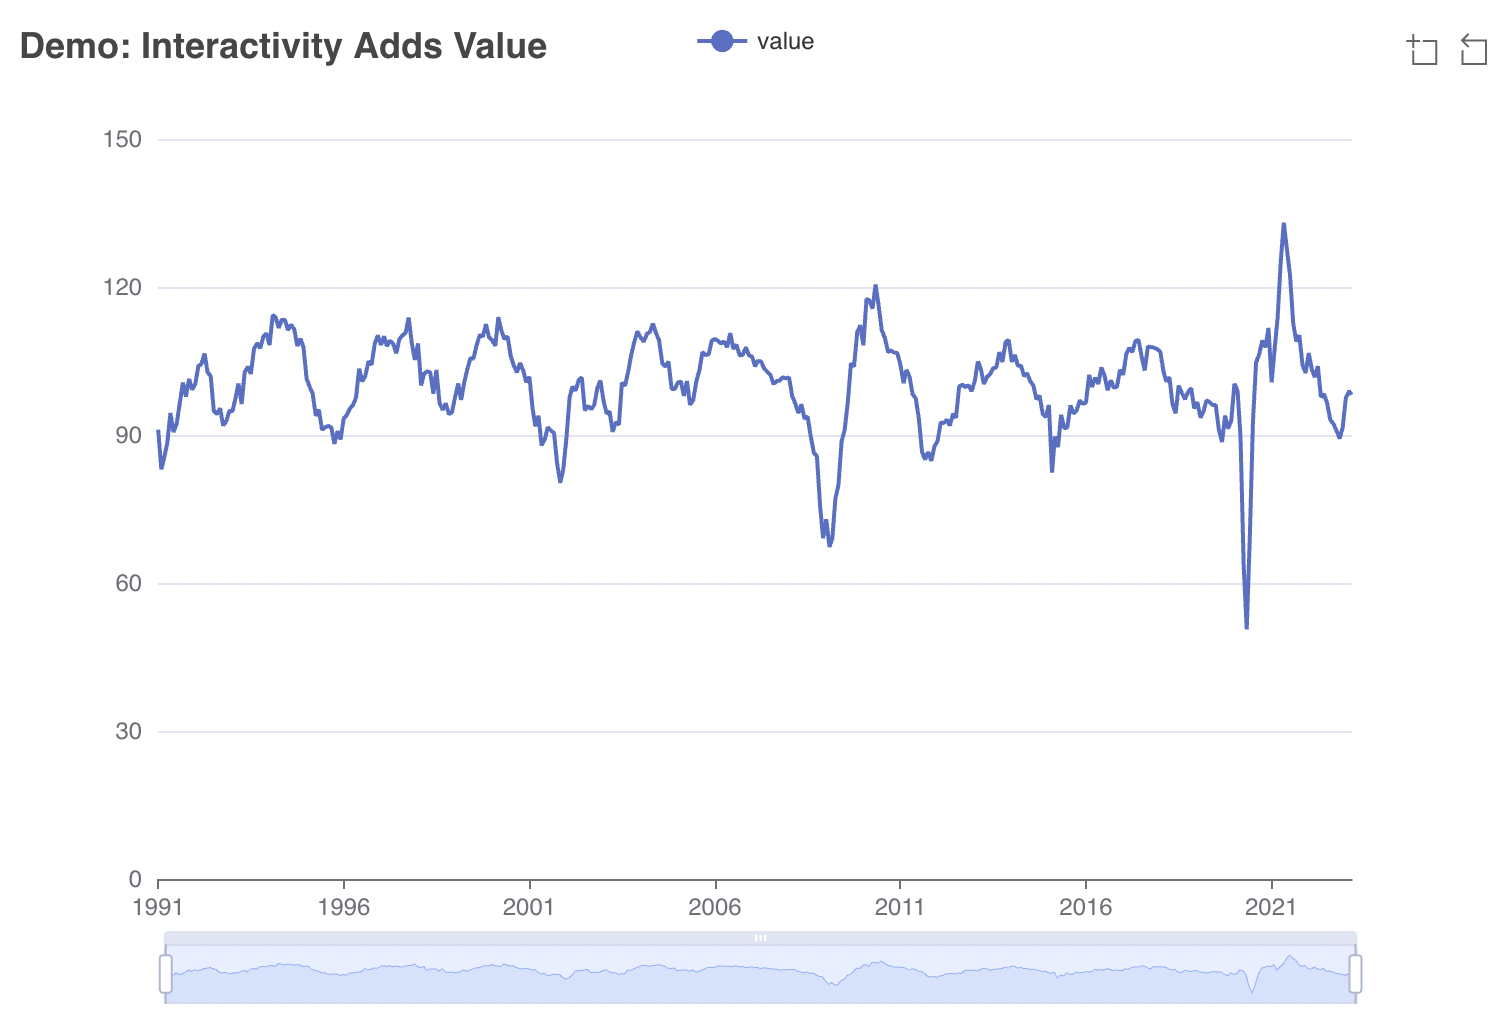
\includegraphics{./images/echart-ts-pdf.png}

}

\caption{Screenshot of an interactive chart created with echarts. Check
the online book for the interactive version:
https://rse-book.github.io/publishing.html\#visualization}

\end{figure}

Besides more universal libraries like D3\index{D3} or echarts with all
their options and opportunities, there are a few smaller libraries that
are much less powerful but a lot simpler to master. Libraries like
\href{}{dygraphs} are limited to, e.g., time series\index{time series}
but are focused on making that one thing as convenient and inclusive as
possible. Depending on your needs, such a smaller library may be an
excellent option. Also, when creating a wrapper package, it is obviously
easier to implement and maintain only a couple of graphics types as
opposed to several hundreds.

\hypertarget{datapub}{%
\section{Data Publications}\label{datapub}}

As mentioned in Chapter~\ref{sec-datamngmnt}, publishing data on
research repositories and catalogs is important not only to make
research reproducible, but to help data workers to get credit for their
contribution to research. Archives like Zenodo\footnote{https://zenodo.org}
provide GitHub integration to automate data releases and versioning of
data. In addition, archives can parse the citation file format
(.cff)\footnote{https://citation-file-format.github.io/} and generate
unique object identification (DOI) numbers for your dataset as well a
meta information for the archive entry. Thanks to rOpenSci, there is
also curated R package called \{cffr\} (Hernangómez 2021) to help
generate citation files.

\bookmarksetup{startatroot}

\hypertarget{case-studies}{%
\chapter{Case Studies}\label{case-studies}}

While the rest of the book provided more of a big
picture\index{big picture} type of insight, this section is all about
application-minded examples that most of the time feature code to
reproduce.

\hypertarget{sec-rsa}{%
\section{SSH Key Pair Authentication}\label{sec-rsa}}

This section could be headed ``log in like a developer''. SSH\index{SSH}
Key Pairs (often referred to as ``RSA key pairs\index{RSA}'' because of
the popular RSA encryption process) are a convenient, relatively secure
way to log into an account. SSH-based connections, including secure copy
(SCP), often make use of SSH Key Pairs instead of using a combination of
username and password. Also, most git platforms use this form of
authentication. The basic idea of key pairs is to have a public key and
a private key. While the private key is never shared with anyone, the
public key is shared with any server you want to log in to. It's like
getting a custom door for any house that you are allowed to enter: share
your public key with the server admin/web portal, and you'll be allowed
in when you show your private key. In case you lose your private key or
suspect it has been stolen, simply inform the admin, so they can remove
the door (public key). This is where a little detail comes into play:
you can password protect the authentication process. Doing so buys you
time to remove the key from the server before your password gets
brute-forced. The downside of this additional password is its need for
interaction. So, when you are setting up a batch that talks to a remote
server, that is when you do \emph{not} want a key without a password.

Step one en route to logging in like a grown up, is to create an RSA key
pair. GitHub\index{GitHub} has a {[}1-2-3 type of manual\footnote{https://docs.github.com/en/free-pro-team@latest/github/authenticating-to-github/generating-a-new-ssh-key-and-adding-it-to-the-ssh-agent}
to get it done. Nevertheless, I would like to show the TL;DR R Studio
(Server) specific way here.

\begin{enumerate}
\def\labelenumi{\arabic{enumi}.}
\tightlist
\item
  Login to your Posit Workbench, RStudio Server or start your Desktop
  RStudio IDE.
\item
  Go to \emph{Tools} → \emph{Global Options} → \emph{Git/SVN}.
\item
  Hit Create RSA KEY (When you have some crazy ASCII art reminiscent of
  a rabbit, it's just ok.)
\item
  Click `View Public Key'.
\item
  Copy this key to your clipboard.
\item
  You can paste the key you obtained to your GitHub\index{GitHub}
  settings or put it into your server's authorized keys file.
\item
  Doing so allows your SSH agent to clone and interact with remote git
  repositories via SSH or log in to a server if your user is allowed to
  use a login shell by the server.
\end{enumerate}

\begin{figure}

{\centering 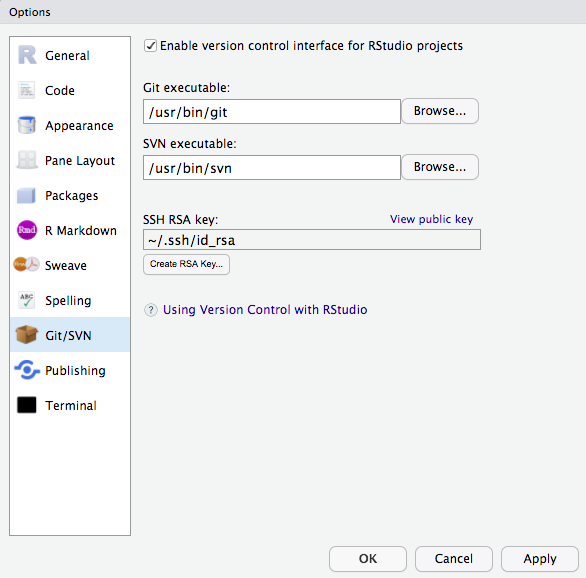
\includegraphics{./images/rsa.png}

}

\caption{The R Studio GUI is an easy way to create a key pair. (Source:
screenshot RStudio IDE taken in 2021.)}

\end{figure}

\hypertarget{application-programming-interfaces}{%
\section{Application Programming
Interfaces}\label{application-programming-interfaces}}

An Application Programming Interface (API)\index{API} is an interface to
facilitate machine-to-machine communication. An interface can be
anything, any protocol or pre-defined process. But, of course, there are
standard and not-so-standard ways to communicate. Plus some
matter-of-taste types of decisions. But security and standard compliance
are none of the latter. There are standards such as the popular,
URL-based REST\index{REST} that make developers' lives a lot easier --
regardless of the language they prefer.

Many services such as Google Cloud, Amazon Webservices (AWS), your
university library, your favorite social media platform or your local
metro operator provide an API. Often, either the platform itself or the
community provides what's called an API wrapper: A simple program wraps
the process of using the interface through dynamic URLs into a
parameterized function. Because the hard work is done server-side by the
API backend, building API wrappers is fairly easy, and, if you're lucky,
wrappers for your favorite languages exit already. If that is the case,
end users can simply use functions like
\texttt{get\_dataset(dataset\_id)} to download data programmatically.

\hypertarget{example-1-the-kofdata-r-package}{%
\subsection{Example 1: The \{kofdata\} R
Package}\label{example-1-the-kofdata-r-package}}

The KOF Swiss Economic Institute at ETH Zurich provides such a wrapper
in the \{kofdata\} R package (Bannert and Thoeni 2022). The underlying
API allows access to the KOF time series\index{time series} archive
database\index{database} and to obtain data and meta information alike.
The below code snippet gets data from the API and uses another KOF built
library (the \{tstools\} R package (Bannert, Thoeni, and Bisinger 2023))
to visualize the returned time series\index{time series}.

\begin{Shaded}
\begin{Highlighting}[]
\FunctionTok{library}\NormalTok{(kofdata)}
\CommentTok{\# just for viz}
\FunctionTok{library}\NormalTok{(tstools)}
\NormalTok{tsl }\OtherTok{\textless{}{-}} \FunctionTok{get\_time\_series}\NormalTok{(}\StringTok{"ch.kof.barometer"}\NormalTok{)}
\FunctionTok{tsplot}\NormalTok{(tsl)}
\end{Highlighting}
\end{Shaded}

\begin{figure}[H]

{\centering 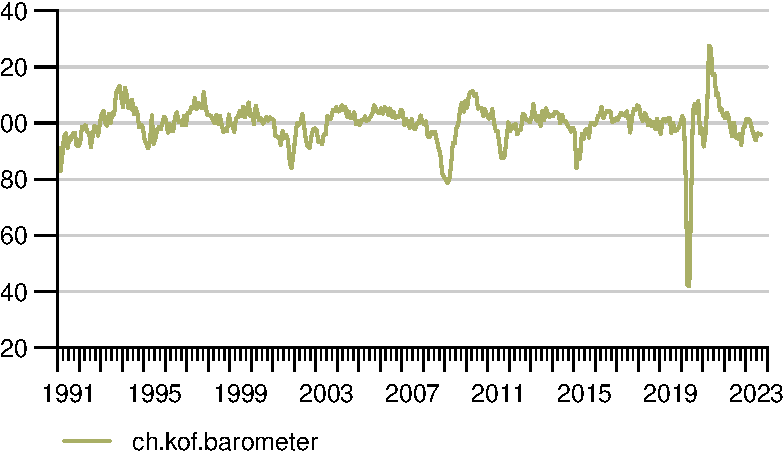
\includegraphics{./case-studies_files/figure-pdf/kofdata-1.pdf}

}

\end{figure}

\hypertarget{build-your-own-api-wrapper}{%
\subsection{\texorpdfstring{Build Your Own API
Wrapper\index{API}}{Build Your Own API Wrapper}}\label{build-your-own-api-wrapper}}

Here's an example of an elementary API\index{API} wrapper that makes use
of the Metropolitan Museum of Modern Art's API to obtain identifiers of
pictures based on a simple search\footnote{Full URL used in the below
  code example:
  https://collectionapi.metmuseum.org/public/collection/v1/search?q=\%s}.

\begin{Shaded}
\begin{Highlighting}[]
\FunctionTok{library}\NormalTok{(jsonlite)}
\CommentTok{\# Visit this example query}
\CommentTok{\# https://collectionapi.metmuseum.org/}
\CommentTok{\# public/collection/v1/search?q=umbrella}
\CommentTok{\# returns a json containing quite a few}
\CommentTok{\# ids of pictures that were tagged \textquotesingle{}umbrella\textquotesingle{}}

\CommentTok{\#\textquotesingle{} Search MET}
\CommentTok{\#\textquotesingle{}}
\CommentTok{\#\textquotesingle{} This function searches the MET\textquotesingle{}s archive}
\CommentTok{\#\textquotesingle{} for keywords and returns object ids of}
\CommentTok{\#\textquotesingle{} search hits. It is a simple wrapper}
\CommentTok{\#\textquotesingle{} around the MET\textquotesingle{}s Application Programming}
\CommentTok{\#\textquotesingle{} interface (API). The function is designed }
\CommentTok{\#\textquotesingle{} to work with other API wrappers}
\CommentTok{\#\textquotesingle{} and use object ids as an input.}
\CommentTok{\#\textquotesingle{} @param character search term}
\CommentTok{\#\textquotesingle{} @return list containing the total }
\CommentTok{\#\textquotesingle{} number of objects found and a }
\CommentTok{\#\textquotesingle{} vector of object ids.}
\CommentTok{\#\textquotesingle{}}
\CommentTok{\# Note these declarations are not relevant}
\CommentTok{\# when code is not part of a package, }
\CommentTok{\# hence you need to call library(jsonlite)}
\CommentTok{\# in order to make this function work if}
\CommentTok{\# you are not building a package.}
\CommentTok{\#\textquotesingle{} @examples}
\CommentTok{\#\textquotesingle{} search\_met("umbrella")}
\CommentTok{\#\textquotesingle{} @importFrom jsonlite formJSON}
\CommentTok{\#\textquotesingle{} @export}
\NormalTok{search\_met }\OtherTok{\textless{}{-}} \ControlFlowTok{function}\NormalTok{(keyword)\{}
  \CommentTok{\# note how URLencode improves this function}
  \CommentTok{\# because spaces are common in searches}
  \CommentTok{\# but are not allowed in URLs}
\NormalTok{  uri }\OtherTok{\textless{}{-}} \StringTok{"https://collect..."}
\NormalTok{  url }\OtherTok{\textless{}{-}} \FunctionTok{sprintf}\NormalTok{(uri,}
  \FunctionTok{URLencode}\NormalTok{(keyword))}
  \FunctionTok{fromJSON}\NormalTok{(url)}
\NormalTok{\}}
\end{Highlighting}
\end{Shaded}

You can use these IDs with another \href{glossary.qmd}{endpoint} to
receive the pictures themselves\footnote{Full URL used in the below code
  example:
  https://collectionapi.metmuseum.org/public/collection/v1/objects/\%d}.

\begin{Shaded}
\begin{Highlighting}[]
\NormalTok{download\_met\_images\_by\_id }\OtherTok{\textless{}{-}} 
  \ControlFlowTok{function}\NormalTok{(ids,}
           \AttributeTok{download =} \StringTok{"primaryImage"}\NormalTok{,}
           \AttributeTok{path =} \StringTok{"met"}\NormalTok{) \{}
  \CommentTok{\# Obtain meta description objects from MET API}
\NormalTok{  obj\_list }\OtherTok{\textless{}{-}} \FunctionTok{lapply}\NormalTok{(ids, }\ControlFlowTok{function}\NormalTok{(x) \{}
\NormalTok{    uri }\OtherTok{\textless{}{-}} \StringTok{"https://collect..."}
\NormalTok{    req }\OtherTok{\textless{}{-}} \FunctionTok{download.file}\NormalTok{(}\FunctionTok{sprintf}\NormalTok{(uri,}
\NormalTok{    x),}\AttributeTok{destfile =} \StringTok{"temp.json"}\NormalTok{)}
    \FunctionTok{fromJSON}\NormalTok{(}\StringTok{"temp.json"}\NormalTok{)}
\NormalTok{  \})}
  
  
\NormalTok{  public }\OtherTok{\textless{}{-}} \FunctionTok{sapply}\NormalTok{(obj\_list, }\StringTok{"[["}\NormalTok{, }\StringTok{"isPublicDomain"}\NormalTok{)}
  
  
  \CommentTok{\# Extract the list elements that contains}
  \CommentTok{\# img URLs in order to pass it to the download function}
\NormalTok{  img\_urls }\OtherTok{\textless{}{-}} \FunctionTok{lapply}\NormalTok{(obj\_list, }\StringTok{"[["}\NormalTok{, download)}
  
  \CommentTok{\# Note the implicit return, no return statement needed}
  \CommentTok{\# last un{-}assigned statement is returned}
  \CommentTok{\# from the function}
  \ControlFlowTok{for}\NormalTok{ (x }\ControlFlowTok{in} \FunctionTok{unlist}\NormalTok{(img\_urls[public]))\{}
    \FunctionTok{download.file}\NormalTok{(x, }\AttributeTok{destfile =} \FunctionTok{sprintf}\NormalTok{(}\StringTok{"\%s/\%s"}\NormalTok{,}
\NormalTok{     path, }\FunctionTok{basename}\NormalTok{(x)))}
\NormalTok{  \}}
  
  
  \FunctionTok{message}\NormalTok{(}
    \FunctionTok{sprintf}\NormalTok{(}\StringTok{"}
\StringTok{    The following images ids were not public}
\StringTok{    domain and could not be downloaded:}\SpecialCharTok{\textbackslash{}n}\StringTok{ \%s"}\NormalTok{,}
            \FunctionTok{paste}\NormalTok{(ids[}\SpecialCharTok{!}\NormalTok{public], }\AttributeTok{collapse =} \StringTok{","}\NormalTok{)}
\NormalTok{  ))}
  
  \FunctionTok{message}\NormalTok{(}
    \FunctionTok{sprintf}\NormalTok{(}\StringTok{"}
\StringTok{    The following images ids were public}
\StringTok{    domain and could be downloaded to}\SpecialCharTok{\textbackslash{}n}\StringTok{ \%s: \%s"}\NormalTok{,}
\NormalTok{            path, }\FunctionTok{paste}\NormalTok{(ids[public], }\AttributeTok{collapse =} \StringTok{","}\NormalTok{)}
\NormalTok{  ))}
  
\NormalTok{\}}
\end{Highlighting}
\end{Shaded}

Finally, execute the functions: first, search for images with umbrellas,
second, download these images by ID. Note that even if I do not display
the image itself in the book to err on the side of caution w.r.t. to
image property rights, the below code shows availability is checked, and
an image is actually downloaded to a previously created folder called
\emph{met}.

\begin{Shaded}
\begin{Highlighting}[]
\CommentTok{\# Step 4: Use the Wrapper}
\NormalTok{umbrella\_ids }\OtherTok{\textless{}{-}} \FunctionTok{search\_met}\NormalTok{(}\StringTok{"umbrella"}\NormalTok{)}
\NormalTok{umbrella\_ids}\SpecialCharTok{$}\NormalTok{total}
\end{Highlighting}
\end{Shaded}

\begin{verbatim}
[1] 722
\end{verbatim}

\begin{Shaded}
\begin{Highlighting}[]
\FunctionTok{head}\NormalTok{(umbrella\_ids}\SpecialCharTok{$}\NormalTok{objectIDs)}
\end{Highlighting}
\end{Shaded}

\begin{verbatim}
[1] 491511  19840  19958   9167 122311 121842
\end{verbatim}

\begin{Shaded}
\begin{Highlighting}[]
\FunctionTok{download\_met\_images\_by\_id}\NormalTok{(umbrella\_ids}\SpecialCharTok{$}\NormalTok{objectIDs[}\DecValTok{30}\SpecialCharTok{:}\DecValTok{33}\NormalTok{])}
\end{Highlighting}
\end{Shaded}

\begin{verbatim}

    The following images ids were not public
    domain and could not be downloaded:
 121919,121922,121809
\end{verbatim}

\begin{verbatim}

    The following images ids were public
    domain and could be downloaded to
 met: 157159
\end{verbatim}

\begin{Shaded}
\begin{Highlighting}[]
\FunctionTok{dir}\NormalTok{(}\StringTok{"met"}\NormalTok{)}
\end{Highlighting}
\end{Shaded}

\begin{verbatim}
character(0)
\end{verbatim}

Wonder what's really in the image? Umbrella or not :) ? Try to reproduce
this example or come up with your own wrapper from scratch \ldots{}

\hypertarget{create-your-own-api}{%
\section{\texorpdfstring{Create Your Own
API\index{API}}{Create Your Own API}}\label{create-your-own-api}}

The ability to expose data is a go-to skill to make research
reproducible and credible. Especially when data get complex and require
thorough description in order to remain reproducible for others, a
programmatic, machine-readable approach is the way to go.

\hypertarget{github-to-serve-static-files}{%
\subsection{\texorpdfstring{GitHub\index{GitHub} to Serve Static
Files\index{static websites}}{GitHub to Serve Static Files}}\label{github-to-serve-static-files}}

Exposing your data through an API is not something for which you would
necessarily need a software engineer, let alone your own server
infrastructure\index{infrastructure} for. Simply hosting a bunch of .csv
spreadsheets alongside a good description (in separate files!!) on,
e.g., GitHub\index{GitHub} for free is an easy and highly available
solution.

The swissdata project\footnote{https://github.com/swissdata} proposes an
implementation of such an approach. The project transforms all sorts of
datasets into .csv spreadsheets to contain a cleaned version of the data
alongside .json files that contain the data descriptions. The
demo\footnote{https://github.com/swissdata/demo} describes the
implementation in a greater detail and hands on fashion.

If you add a naming convention for your files to such an implementation,
you already have a solid interface to a data science environment.
Consider the following simple R wrapper that downloads both data and
metadata first and then reads both into R\footnote{Full URL of the below
  code example:
  https://raw.githubusercontent.com/swissdata/demo/master/data}.
(Alternatively, direct streaming would be possible, too.)

\begin{Shaded}
\begin{Highlighting}[]
\FunctionTok{library}\NormalTok{(jsonlite)}
\NormalTok{download\_swissdata }\OtherTok{\textless{}{-}} \ControlFlowTok{function}\NormalTok{(dataset)\{}
\NormalTok{  d\_ext }\OtherTok{\textless{}{-}} \StringTok{".csv"}  
\NormalTok{  m\_ext }\OtherTok{\textless{}{-}} \StringTok{".json"}
\NormalTok{  d }\OtherTok{\textless{}{-}} \FunctionTok{sprintf}\NormalTok{(}\StringTok{"\%s\%s"}\NormalTok{, dataset, d\_ext)}
\NormalTok{  m }\OtherTok{\textless{}{-}} \FunctionTok{sprintf}\NormalTok{(}\StringTok{"\%s\%s"}\NormalTok{, dataset, m\_ext)}
\NormalTok{  gh\_url }\OtherTok{\textless{}{-}} \StringTok{"https://raw.git..."}\ErrorTok{)}
  \FunctionTok{download.file}\NormalTok{(}\FunctionTok{file.path}\NormalTok{(gh\_url, d), d)}
  \FunctionTok{download.file}\NormalTok{(}\FunctionTok{file.path}\NormalTok{(gh\_url, m), m)}
\NormalTok{\}}


\FunctionTok{download\_swissdata}\NormalTok{(}\StringTok{"ch\_adecco\_sjmi"}\NormalTok{)}
\end{Highlighting}
\end{Shaded}

Now, read the data from disk into your R session

\begin{Shaded}
\begin{Highlighting}[]
\NormalTok{d }\OtherTok{\textless{}{-}} \FunctionTok{read.csv}\NormalTok{(}\StringTok{"ch\_adecco\_sjmi.csv"}\NormalTok{)}
\FunctionTok{head}\NormalTok{(d)}
\end{Highlighting}
\end{Shaded}

\begin{verbatim}
  idx_type       date value
1      sch 2003-03-01  31.9
2     pzua 2003-03-01  12.9
3      ins 2003-03-01   4.9
4      unw 2003-03-01  14.2
5      sch 2004-03-01  36.4
6     pzua 2004-03-01  12.2
\end{verbatim}

As well as the nested meta information\{nested data\}. JSON maps 1:1 to
R lists. Hence, both the on-disk representation and the
in-memory\index{in-memory} representation are equally well suited for
nested data. The below example shows a sub-label element containing
description in multiple languages.

\begin{Shaded}
\begin{Highlighting}[]
\NormalTok{m }\OtherTok{\textless{}{-}} \FunctionTok{fromJSON}\NormalTok{(}\StringTok{"ch\_adecco\_sjmi.json"}\NormalTok{)}
\NormalTok{m}\SpecialCharTok{$}\NormalTok{labels}\SpecialCharTok{$}\NormalTok{idx\_type}\SpecialCharTok{$}\NormalTok{unw}
\end{Highlighting}
\end{Shaded}

\begin{verbatim}
$en
[1] "Company websites"

$de
[1] "Unternehmens-Webseiten"

$fr
named list()

$it
named list()
\end{verbatim}

\begin{tcolorbox}[enhanced jigsaw, left=2mm, arc=.35mm, colbacktitle=quarto-callout-note-color!10!white, breakable, colframe=quarto-callout-note-color-frame, bottomrule=.15mm, bottomtitle=1mm, colback=white, leftrule=.75mm, coltitle=black, toptitle=1mm, titlerule=0mm, title=\textcolor{quarto-callout-note-color}{\faInfo}\hspace{0.5em}{Note}, opacityback=0, rightrule=.15mm, toprule=.15mm, opacitybacktitle=0.6]

Note, standard GitHub\index{GitHub} repositories are not well suited to
host larger files or binaries. Check out their file hosting offering or
consider other services focused on files.

\end{tcolorbox}

\hypertarget{simple-dynamic-apis}{%
\subsection{\texorpdfstring{Simple Dynamic
APIs\index{API}}{Simple Dynamic APIs}}\label{simple-dynamic-apis}}

Even, going past serving static files, does not require much software
development expertise. Thanks to frameworks such as express.js or the
\{plumbr\} package in the R ecosystem, it is easy to create an API that
turns an URL into a parameterized server-side action. Before we look at
one of those frameworks in greater detail, let's take a look at the two
most common HTTP request methods\footnote{https://developer.mozilla.org/en-US/docs/Web/HTTP/Methods}
GET and POST.

According to Mozilla's definition, the GET method ``requests a
representation of the specified resource. Requests using GET should only
retrieve data,'' while POST ``submits an entity to the specified
resource, often causing a change in state or side effects on the
server''. Obviously, there are many other methods for the HTTP protocol,
but the above two should help to understand the idea behind standard
compliant REST\index{REST} web application programming interfaces.

Let's assume you have a working nodejs\footnote{https://nodejs.org/en/}
JavaScript\index{JavaScript} runtime environment installed on your local
development machine, so you can run JavaScript files outside a web
browser. Such a setup mimics the situation on a web server with Node.js
installed. Also, let's assume you have npm\footnote{https://npmjs.com}
installed as a package manager to facilitate installing node packages
from the npm open source package registry.

First, create a folder \texttt{api}, go to the freshly created directory
and initiate a node package.

\begin{verbatim}
# run initialization in a dedicated folder
mkdir api
cd api
mkdir public 
npm init
\end{verbatim}

Just sleepwalk through the interactive dialog accepting all defaults.
This created a package.json file to keep track of dependencies and their
package versions used in your project. Once done, add express using the
npm package manager.

\begin{verbatim}
npm install express
\end{verbatim}

Now, that we installed the JavaScript framework Express.js, we can use
the framework to create a minimal web application that serves an API
endpoint using the node runtime environment. Consider a minimal
hello-world example that does about the same as the static file example
of the previous action:

\begin{Shaded}
\begin{Highlighting}[]
\KeywordTok{const}\NormalTok{ express }\OperatorTok{=} \PreprocessorTok{require}\NormalTok{(}\StringTok{\textquotesingle{}express\textquotesingle{}}\NormalTok{)}
\KeywordTok{const}\NormalTok{ app }\OperatorTok{=} \FunctionTok{express}\NormalTok{()}
\KeywordTok{const}\NormalTok{ port }\OperatorTok{=} \DecValTok{3000}

\NormalTok{app}\OperatorTok{.}\FunctionTok{get}\NormalTok{(}\StringTok{\textquotesingle{}/\textquotesingle{}}\OperatorTok{,}\NormalTok{ (req}\OperatorTok{,}\NormalTok{ res) }\KeywordTok{=\textgreater{}}\NormalTok{ \{}
\NormalTok{  res}\OperatorTok{.}\FunctionTok{send}\NormalTok{(}\StringTok{\textquotesingle{}Hello World!\textquotesingle{}}\NormalTok{)}
\NormalTok{\})}

\NormalTok{app}\OperatorTok{.}\FunctionTok{use}\NormalTok{(}\StringTok{\textquotesingle{}/static\textquotesingle{}}\OperatorTok{,}\NormalTok{ express}\OperatorTok{.}\FunctionTok{static}\NormalTok{(}\StringTok{\textquotesingle{}public\textquotesingle{}}\NormalTok{))}


\NormalTok{app}\OperatorTok{.}\FunctionTok{listen}\NormalTok{(port}\OperatorTok{,}\NormalTok{ () }\KeywordTok{=\textgreater{}}\NormalTok{ \{}
  \BuiltInTok{console}\OperatorTok{.}\FunctionTok{log}\NormalTok{(}\VerbatimStringTok{\textasciigrave{}RSE demo app listening on port }\SpecialCharTok{$\{}\NormalTok{port}\SpecialCharTok{\}}\VerbatimStringTok{\textasciigrave{}}\NormalTok{)}
\NormalTok{\})}
\end{Highlighting}
\end{Shaded}

The first \texttt{app.get} route simply maps the root, a plain,
un-nested starting point so to say, in our case \texttt{localhost:3000/}
to the output of the \texttt{res.send} call. The second \texttt{app}
command serves the content of the \texttt{public} folder to visitor's of
\texttt{localhost:3000/static}. So if a \texttt{public/} folder inside
the app folder contained a cover image of my \emph{Hacking for Science}
courses, this would be served at
\texttt{localhost:3000/static/h4sci.jpeg}.

\begin{figure}

{\centering 
\includegraphics{./images/h4sci.png}

}

\caption{Cover illustration of the Hacking for Science Courses. (Source:
own illustration.)}

\end{figure}

Now let us make use of server-side features beyond simply serving static
files and add the need for an API key to get the picture.

\begin{Shaded}
\begin{Highlighting}[]
\KeywordTok{const}\NormalTok{ express }\OperatorTok{=} \PreprocessorTok{require}\NormalTok{(}\StringTok{\textquotesingle{}express\textquotesingle{}}\NormalTok{)}
\KeywordTok{const}\NormalTok{ app }\OperatorTok{=} \FunctionTok{express}\NormalTok{()}
\KeywordTok{const}\NormalTok{ port }\OperatorTok{=} \DecValTok{3000}

\NormalTok{app}\OperatorTok{.}\FunctionTok{get}\NormalTok{(}\StringTok{\textquotesingle{}/\textquotesingle{}}\OperatorTok{,}\NormalTok{ (req}\OperatorTok{,}\NormalTok{ res) }\KeywordTok{=\textgreater{}}\NormalTok{ \{}
\NormalTok{  res}\OperatorTok{.}\FunctionTok{send}\NormalTok{(}\StringTok{\textquotesingle{}Hello World!\textquotesingle{}}\NormalTok{)}
\NormalTok{\})}

\NormalTok{app}\OperatorTok{.}\FunctionTok{use}\NormalTok{(}\StringTok{\textquotesingle{}/static\textquotesingle{}}\OperatorTok{,}\NormalTok{ (req}\OperatorTok{,}\NormalTok{ res}\OperatorTok{,}\NormalTok{ next) }\KeywordTok{=\textgreater{}}\NormalTok{ \{  }
  \KeywordTok{var}\NormalTok{ key }\OperatorTok{=}\NormalTok{ req}\OperatorTok{.}\AttributeTok{query}\NormalTok{[}\StringTok{\textquotesingle{}api\_key\textquotesingle{}}\NormalTok{]}\OperatorTok{;}
  \ControlFlowTok{if}\NormalTok{ (}\OperatorTok{!}\NormalTok{key) res}\OperatorTok{.}\FunctionTok{send}\NormalTok{(}\StringTok{\textquotesingle{}api key required\textquotesingle{}}\NormalTok{)}\OperatorTok{;}
  \ControlFlowTok{if}\NormalTok{ (apiKeys}\OperatorTok{.}\FunctionTok{indexOf}\NormalTok{(key) }\OperatorTok{===} \OperatorTok{{-}}\DecValTok{1}\NormalTok{)  res}\OperatorTok{.}\FunctionTok{send}\NormalTok{(}\StringTok{\textquotesingle{}eh{-}eh,}
\NormalTok{   wrong key}\OperatorTok{.}\StringTok{\textquotesingle{});}
\NormalTok{  req}\OperatorTok{.}\AttributeTok{key} \OperatorTok{=}\NormalTok{ key}\OperatorTok{;}
  \FunctionTok{next}\NormalTok{()}\OperatorTok{;}
\NormalTok{\})}


\CommentTok{// }\AlertTok{NOTE}\CommentTok{ THAT this is only a }
\CommentTok{// demo example (!)}
\CommentTok{// DO NOT use insecure passwords}
\CommentTok{// in production.}
\CommentTok{// Make sure to find better ways}
\CommentTok{// to secure your keys! }
\CommentTok{// also transferring keys in URLs}
\CommentTok{// via GET is not optimal, }
\CommentTok{// consider using an upfront}
\CommentTok{// authentication method}
\KeywordTok{var}\NormalTok{ apiKeys }\OperatorTok{=}\NormalTok{ [}\StringTok{\textquotesingle{}abc\textquotesingle{}}\OperatorTok{,}\StringTok{\textquotesingle{}123\textquotesingle{}}\NormalTok{]}\OperatorTok{;}
\NormalTok{app}\OperatorTok{.}\FunctionTok{use}\NormalTok{(}\StringTok{\textquotesingle{}/static\textquotesingle{}}\OperatorTok{,}\NormalTok{ express}\OperatorTok{.}\FunctionTok{static}\NormalTok{(}\StringTok{\textquotesingle{}public\textquotesingle{}}\NormalTok{))}

\NormalTok{app}\OperatorTok{.}\FunctionTok{listen}\NormalTok{(port}\OperatorTok{,}\NormalTok{ () }\KeywordTok{=\textgreater{}}\NormalTok{ \{}
  \BuiltInTok{console}\OperatorTok{.}\FunctionTok{log}\NormalTok{(}\VerbatimStringTok{\textasciigrave{}RSE demo api listening on port }\SpecialCharTok{$\{}\NormalTok{port}\SpecialCharTok{\}}\VerbatimStringTok{\textasciigrave{}}\NormalTok{)}
\NormalTok{\})}
\end{Highlighting}
\end{Shaded}

We simply added a mount point using \texttt{app.use} (instead of
\texttt{app.get}) which makes sure that everything past \texttt{/static}
is affected by the logic added to this mount. So, our
\texttt{Hello\ World!} greeting is out there for anybody to see, while
displaying the picture whose URL starts with \texttt{/static} needs an
API key. Though this is only one, admittedly made up example of mapping
URLs and parameters to functions via HTTP(S), it hints at the
possibilities of dynamic APIs from database\index{database} queries to
web forms and many other applications. The above example shows also how
frameworks like Express JavaScript\footnote{https://expressjs.com/} or
plumber (Schloerke and Allen 2022) facilitate the definition of
machine-to-machine interfaces even for less experienced developers. The
impact of frameworks is not limited to the technical implementation,
though. Developers benefit from comprehensive approaches like Swagger
and the OpenAPI specification during the conceptual part of creating
machine to machine interfaces.

\hypertarget{sec-webscrape}{%
\section{\texorpdfstring{A Minimal Webscraper\index{webscraping}:
Extracting Publication
Dates}{A Minimal Webscraper: Extracting Publication Dates}}\label{sec-webscrape}}

Even though KOF Swiss Economic Institute offers a REST API to consume
publicly available data, publication dates are unfortunately not
available through in API just yet. Hence, to automate data consumption
based on varying publication dates, we need to extract upcoming
publication dates of the Barometer from KOF's media release calendar.
Fortunately, all future releases are presented online in an
easy-to-scrape table. So, here's the plan:

\begin{enumerate}
\def\labelenumi{\arabic{enumi}.}
\item
  Use Google Chrome's \emph{inspect element} developer feature to find
  the X-Path (location in the Document Object Model) of the table.
\item
  Read the web page into R using \texttt{rvest}.
\item
  Copy the X-Path string to R to turn the table into a data.frame
\item
  Use a regular expression to filter the description for what we need.
\end{enumerate}

First, let's take a look at our starting point, the media releases
sub-page, first.

\begin{figure}

{\centering 
\includegraphics{./images/agenda.png}

}

\caption{The KOF Swiss Economic Institute's media agenda in 2021.
(Source: screenshot Google Chrome browser.)}

\end{figure}

The website looks fairly simple, and the jackpot is not hard, presented
in a table right in front of us. Can't you smell the data.frame already?

Right-click the table to see a Chrome context window pop up. Select
\emph{inspect}.

\begin{figure}

{\centering 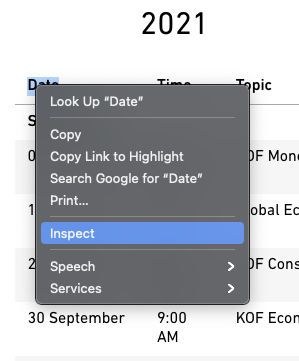
\includegraphics{./images/inspect.png}

}

\caption{Modern browsers come with developer tools built in to help you
expect a website's source code. (Source: screenshot Google Chrome
browser.)}

\end{figure}

Hover over the highlighted line in the source code at the bottom. Make
sure the selected line marks the table. Right click again, select copy →
copy X-Path\footnote{Full URL used in the below code example:
  https://kof.ethz.ch/news-und-veranstaltungen/medien/medienagenda.html}.

\begin{figure}

{\centering 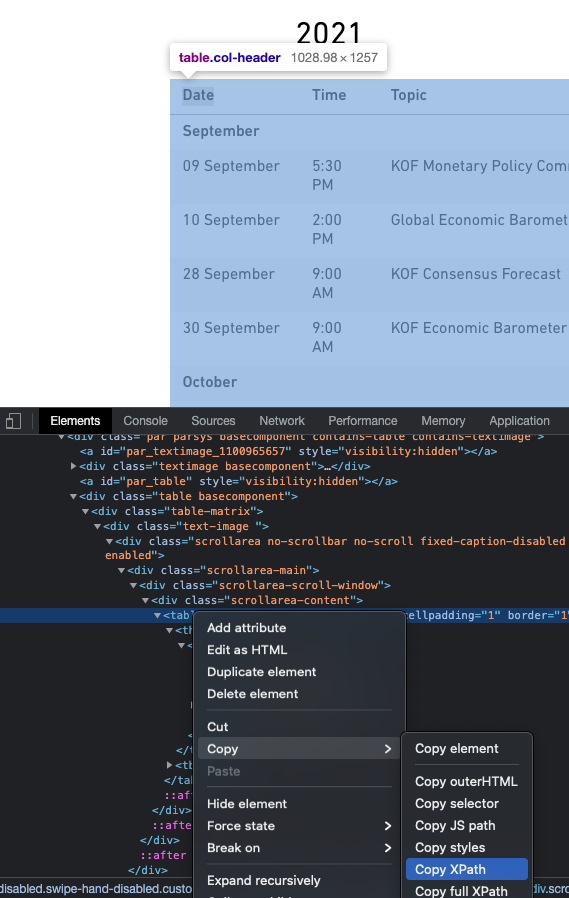
\includegraphics{./images/xpath.png}

}

\caption{Browser tools help you explore the hierarchical structure of a
website in interactive fashion. (Source: screenshot Google Chrome
browser.)}

\end{figure}

On to R!

\begin{Shaded}
\begin{Highlighting}[]
\FunctionTok{library}\NormalTok{(rvest)}
\CommentTok{\# URL of the media release subsite}
\NormalTok{url }\OtherTok{\textless{}{-}} \StringTok{"https://kof.ethz.ch..."}
\CommentTok{\# Extract the DOM object from the path we\textquotesingle{}ve }
\CommentTok{\# previously detected using }
\CommentTok{\# Chrome\textquotesingle{}s inspect feature}
\NormalTok{table\_list }\OtherTok{\textless{}{-}}\NormalTok{ url }\SpecialCharTok{\%\textgreater{}\%}
  \FunctionTok{read\_html}\NormalTok{() }\SpecialCharTok{\%\textgreater{}\%}
  \FunctionTok{html\_nodes}\NormalTok{(}\AttributeTok{xpath =} \StringTok{\textquotesingle{}}
\StringTok{  //html/body/div[6]/section/div/section}
\StringTok{  /div[2]/div/div[3]/div/div/div/}
\StringTok{  div/div/div/div/table\textquotesingle{}}\NormalTok{) }\SpecialCharTok{\%\textgreater{}\%}
  \CommentTok{\# turn the HTML table into an R data.frame}
  \FunctionTok{html\_table}\NormalTok{()}
\CommentTok{\# because the above result may potentially contain}
\CommentTok{\# multiple tables, we just use }
\CommentTok{\# the first table. We know from visual}
\CommentTok{\# inspection of the site that this is the}
\CommentTok{\# right table. }
\NormalTok{agenda\_table }\OtherTok{\textless{}{-}}\NormalTok{ table\_list[[}\DecValTok{1}\NormalTok{]]}

\CommentTok{\# *[@id="t{-}6b2da0b4{-}cec0{-}47a4{-}bf9d{-}}
\CommentTok{\#   bbfa5338fec8{-}tbody{-}row{-}2{-}cell{-}2"]}

\CommentTok{\# extract KOF barometer lines}
\NormalTok{pub\_date }\OtherTok{\textless{}{-}}\NormalTok{ agenda\_table[}\FunctionTok{grep}\NormalTok{(}\StringTok{"barometer"}\NormalTok{,}
\NormalTok{                         agenda\_table}\SpecialCharTok{$}\NormalTok{X3),]}
\NormalTok{pub\_date}
\end{Highlighting}
\end{Shaded}

Yay! We got everything we wanted. Ready to process.

\hypertarget{automate-script-execution-an-example-with-github-actions}{%
\section{\texorpdfstring{Automate Script Execution: An Example with
GitHub\index{GitHub}
Actions\index{CI/CD}}{Automate Script Execution: An Example with GitHub Actions}}\label{automate-script-execution-an-example-with-github-actions}}

containerization\index{containerization} as described in the
infrastructure\index{infrastructure} section has standardized virtual
hardware into building blocks that are available across different
platforms and providers. This development has led to a wide array of
offerings that allow us to run our code in a language-agnostic
environment. In addition to the major cloud platforms, git providers
that offer a CI/CD\index{CI/CD} tool chain are a good option to run our
code on a remote container\index{container}. Though originally designed
mostly for build automation\index{automation}, CI/CD\index{CI/CD} such
as GitHub actions can be used to automate a variety of tasks by running
them on a container\index{container}. Consider the following minimal R
script that we will run on GitHub\index{GitHub} actions.

\begin{Shaded}
\begin{Highlighting}[]
\CommentTok{\#!/usr/bin/env Rscript}

\FunctionTok{library}\NormalTok{(knitr)}
\FunctionTok{knit}\NormalTok{(}\StringTok{"README.Rmd"}\NormalTok{)}
\end{Highlighting}
\end{Shaded}

The script uses \{knitr\} to render an RMarkdown document to a Markdown
document that is automatically rendered to a pretty HTML file when
pushed to a repository hosted on GitHub\index{GitHub}.

\begin{tcolorbox}[enhanced jigsaw, left=2mm, arc=.35mm, colbacktitle=quarto-callout-note-color!10!white, breakable, colframe=quarto-callout-note-color-frame, bottomrule=.15mm, bottomtitle=1mm, colback=white, leftrule=.75mm, coltitle=black, toptitle=1mm, titlerule=0mm, title=\textcolor{quarto-callout-note-color}{\faInfo}\hspace{0.5em}{Note}, opacityback=0, rightrule=.15mm, toprule=.15mm, opacitybacktitle=0.6]

Notice the common \emph{shebang} comment that defines the executable for
batch execution of a script file -- in this case \emph{Rscript} to run R
outside of an interactive R session.

\end{tcolorbox}

Embedded in a bit of descriptive text before and after the code, the
main code chunk of the .Rmd template file is equally straightforward:

\begin{Shaded}
\begin{Highlighting}[]
\FunctionTok{library}\NormalTok{(kofdata)}
\FunctionTok{library}\NormalTok{(tsbox)}
\NormalTok{tsl }\OtherTok{\textless{}{-}} \FunctionTok{get\_time\_series}\NormalTok{(}\StringTok{"ch.kof.barometer"}\NormalTok{)}
\FunctionTok{ts\_plot}\NormalTok{(tsl}\SpecialCharTok{$}\NormalTok{ch.kof.barometer)}
\FunctionTok{cat}\NormalTok{(}\FunctionTok{sprintf}\NormalTok{(}\StringTok{"last update on \%s."}\NormalTok{,}
 \FunctionTok{as.character}\NormalTok{(}\FunctionTok{Sys.Date}\NormalTok{())))}
\end{Highlighting}
\end{Shaded}

We make use of the \{kofdata\} API wrapper to obtain data from the KOF
Data API and use the \{tsbox\} to visualize the time
series\index{time series} data we received. Finally, we print the system
date of the runtime environment -- in our case the GitHub Actions
Docker\index{Docker} container. Running the README.\textbf{Rmd} file
yields two artifacts: (1) a README.\textbf{md} file and a (2) .png graph
located in a \texttt{figure/} folder. Because the above runs inside a
temporary single purpose container, our workflow needs to make sure
those artifacts are stored persistently.

The below .yaml file defines the environment and workflow for GitHub
Actions. When located properly according to GitHub's\index{GitHub}
convention, i.e., in a hidden \texttt{github/worflows} folder, GitHub
identifies the .yaml file as input and allows executing the workflow.
(Standalone build tools like Woodpecker\index{Woodpecker} or other
integrated CI/CD\index{CI/CD} tools like GitLab\index{GitLab}
CI/CD\index{CI/CD} use very similar workflow definitions).

\begin{Shaded}
\begin{Highlighting}[]
\CommentTok{\# Simple data transformation workflow}
\FunctionTok{name}\KeywordTok{:}\AttributeTok{ KOF Economic Barometer}

\CommentTok{\# Controls when the action will run. }
\CommentTok{\# Triggers the workflow on push or pull request}
\CommentTok{\# events but only for the main branch}
\FunctionTok{on}\KeywordTok{:}
\AttributeTok{  workflow\_dispatch}

\FunctionTok{jobs}\KeywordTok{:}
\AttributeTok{  }\FunctionTok{kof}\KeywordTok{:}
\AttributeTok{    }\FunctionTok{runs{-}on}\KeywordTok{:}\AttributeTok{ ubuntu{-}latest}
\AttributeTok{    }\FunctionTok{container}\KeywordTok{:}\AttributeTok{ rocker/verse}
\AttributeTok{    }\FunctionTok{steps}\KeywordTok{:}
\AttributeTok{      }\KeywordTok{{-}}\AttributeTok{ }\FunctionTok{uses}\KeywordTok{:}\AttributeTok{ actions/checkout@v3}
\AttributeTok{      }\KeywordTok{{-}}\AttributeTok{ }\FunctionTok{run}\KeywordTok{:}\AttributeTok{ git version}
\AttributeTok{      }\KeywordTok{{-}}\AttributeTok{ }\FunctionTok{run}\KeywordTok{:}\AttributeTok{ rm {-}rf README.md}
\KeywordTok{      {-} }\FunctionTok{run}\KeywordTok{:}\AttributeTok{ }\CharTok{|}
\NormalTok{          Rscript {-}e \textbackslash{} }
\NormalTok{          \&\& \textquotesingle{}install.packages(c("kofdata","tsbox"))\textquotesingle{}}
\NormalTok{          chmod +x demo\_gha.R}
\NormalTok{          ./demo\_gha.R}
\AttributeTok{      }\KeywordTok{{-}}\AttributeTok{ }\FunctionTok{run}\KeywordTok{:}\AttributeTok{ ls {-}lah}
\KeywordTok{      {-} }\FunctionTok{run}\KeywordTok{:}\AttributeTok{ }\CharTok{|}
\NormalTok{          git config {-}{-}global {-}{-}add safe.directory \textbackslash{}}
\NormalTok{          \&\& /\_\_w/h4sci{-}gha{-}demo/h4sci{-}gha{-}demo}
\NormalTok{          git config {-}{-}global user.name \textbackslash{}}
\NormalTok{          \&\& "Matt Bannert"}
\NormalTok{          git config {-}{-}global user.email \textbackslash{}}
\NormalTok{          \&\& "mbannert@users.noreply.github.com"}
\NormalTok{          git add figure README.md}
\NormalTok{          git commit {-}m \textbackslash{}}
\NormalTok{          \&\& "Update README.md via GH Actions"}
\NormalTok{          git push}
\end{Highlighting}
\end{Shaded}

First, the below file gives our workflow a name to identify the workflow
among other workflows defined within the same repository. The
\texttt{on} block defines what triggers the workflow. The
\texttt{workflow\_dispatch} option is a rather uncommon trigger, as it
simply means the workflow can be triggered by pressing a button in
GitHub's Web GUI. Cronjob-based triggers or triggers based on git
actions such as pushes to a certain branch are more common as we are
looking to avoid interaction at runtime. Inside the job definitions
itself, we first define the operating system of the host and the
Docker\index{Docker} image in which our process should run.

Then, walk through the single steps of our workflow. Notice that
\texttt{actions/checkout@v3} is different from the other steps because
it is taken from GitHub's marketplace for actions. Instead of writing
standard operations, namely checking out the git repository we're
working with to the container that runs the action, from scratch, we use
the marketplace action for that. Be aware though that there is a
trade-off between convenience and transparency. When I was teaching this
year and wanted to recycle an example from the previous year, it was not
all that convenient. Only one year later, my example that leaned heavily
on marketplace actions was not working anymore. What's worse is that it
was also relatively hard to debug because I had to deal with the inner
workings of a dependency heavy implementation that I would not have
implemented this way. If we look at the above steps after the checkout
action, we see a list of simple steps that are easy to read: first,
simply print the git version to make sure git is working inside the
container, and we know its version in case we need to debug. Second, we
remove the README.md file we have just checked out. This file will be
replaced anyway, and we want to avoid any rights conflicts overwriting
the file. Then we run R in batch to install two more specific packages
to the R environment running inside the container. Because we use a
pre-built \emph{tidyverse} images from the rocker project, we do not
have to install R itself and many common packages. We continue to use
the \emph{chmod} Linux command to change the access rights of our
minimal R script. With the \emph{shebang} comment inside the file, we
can directly execute the .R file with the \texttt{./} prefix because it
knows which executable to use to run it. Finally, we take a look at the
content of the current folder before we commit and push all the files we
generated back to our GitHub repository. After the process is done, the
container will stop and removed.

\begin{tcolorbox}[enhanced jigsaw, left=2mm, arc=.35mm, colbacktitle=quarto-callout-note-color!10!white, breakable, colframe=quarto-callout-note-color-frame, bottomrule=.15mm, bottomtitle=1mm, colback=white, leftrule=.75mm, coltitle=black, toptitle=1mm, titlerule=0mm, title=\textcolor{quarto-callout-note-color}{\faInfo}\hspace{0.5em}{Note}, opacityback=0, rightrule=.15mm, toprule=.15mm, opacitybacktitle=0.6]

Note that we can see all the output of the process from the
GitHub\index{GitHub} actions menu on our repository's website. This is
why it's useful to print outputs of intermediate steps.

\end{tcolorbox}

\hypertarget{sec-map}{%
\section{\texorpdfstring{Choropleth Map: Link Data to a
GeoJSON\index{GeoJSON} Map
File}{Choropleth Map: Link Data to a GeoJSON Map File}}\label{sec-map}}

\begin{figure}

{\centering 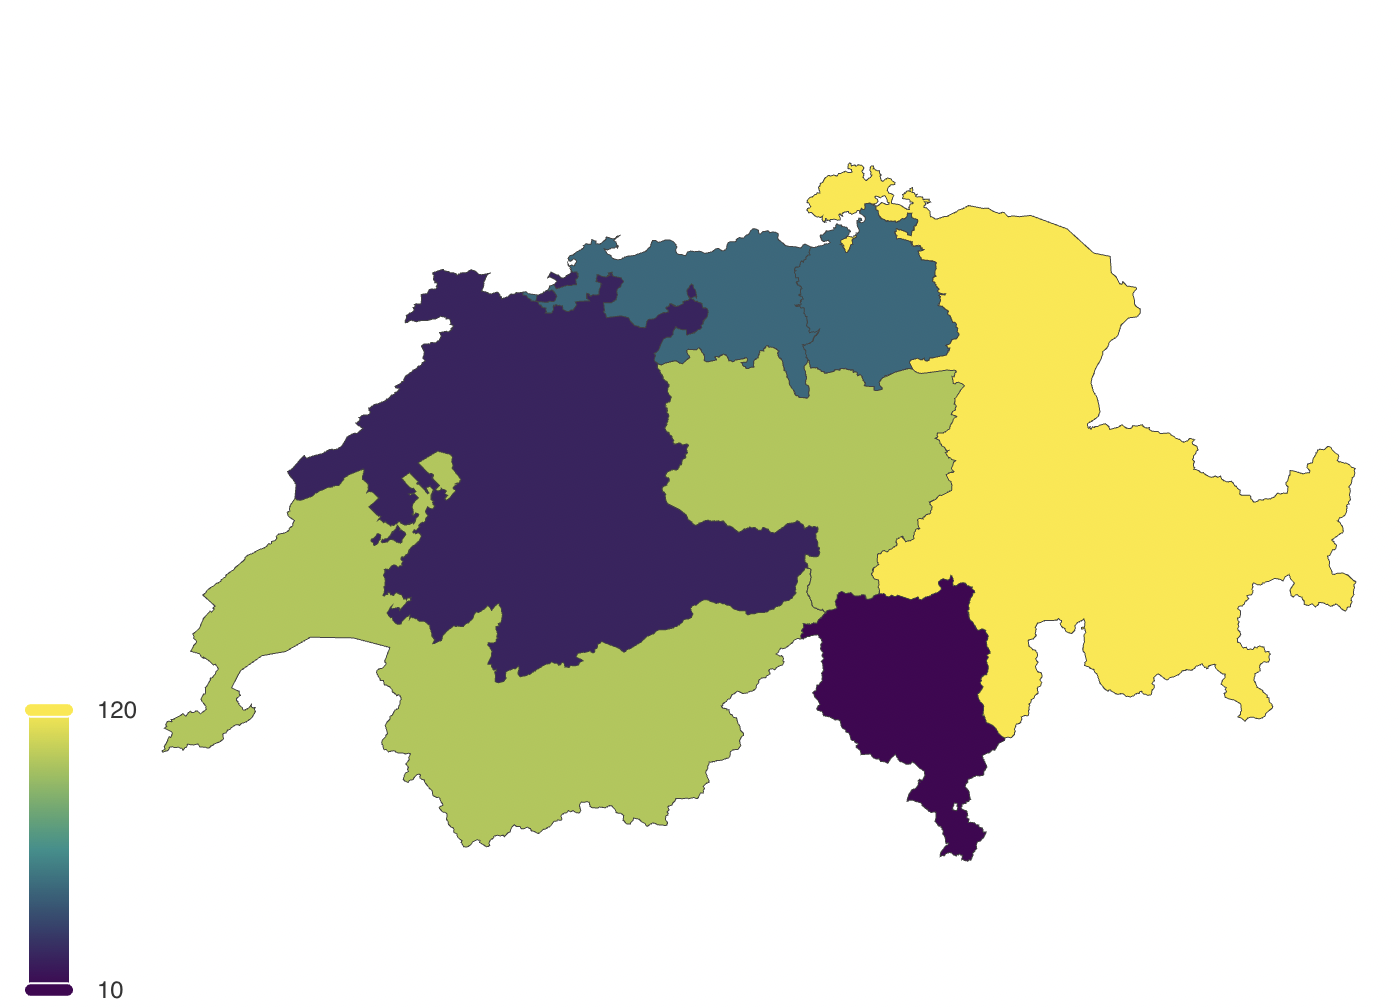
\includegraphics{./images/case-choropleth.png}

}

\caption{Screenshot of an interactive choropleth; for the actual,
interactive visit https://rse-book.github.io/case-studies.html\#sec-map}

\end{figure}

Data visualization is a big reason for researchers and data analysts to
look into programming languages. Programming languages do not only
provide unparalleled flexibility, but they also make data visualization
reproducible and allow placing charts in different contexts, e.g.,
websites, printed outlets or social media.

One of the more popular types of plots that can be created smoothly
using a programming language is the so-called
\emph{choropleth}\index{choropleth}. A \emph{choropleth} maps values of
a variable that is available by region to a given continuous color
palette on a map. Let's break down the ingredients of the below map of
Switzerland\footnote{Full URL used in the below example
  https://raw.githubusercontent.com/mbannert/maps/master/ch\_bfs\_regions.geojson}.

First, we need a \emph{definition of a country's shape}. Those
definitions come in various formats, from traditional \emph{shape files}
to web-friendly \emph{GeoJSON}. Edzer Pebesma's useR! 2021
keynote\footnote{https://www.youtube.com/watch?v=cK08bxUJn5A} has a more
thorough insight.

Second, we need some data.frame that simply connects values to regions.
In this case, we use regions defined by the Swiss Federal Statistical
Office (FSO). Because our charting library makes use of the
GeoJSON\index{GeoJSON} convention to call the region label ``name'' we
need to call the column that holds the region names ``name'' as well.
That way, we can safely use defaults when plotting. Ah, and note that
the values are absolutely bogus that came to my mind while writing this
(so please do not mull over how these values were picked).

\begin{Shaded}
\begin{Highlighting}[]
\NormalTok{d }\OtherTok{\textless{}{-}} \FunctionTok{data.frame}\NormalTok{(}
  \AttributeTok{name =} \FunctionTok{c}\NormalTok{(}\StringTok{"Zürich"}\NormalTok{,}
           \StringTok{"Ticino"}\NormalTok{,}
           \StringTok{"Zentralschweiz"}\NormalTok{,}
           \StringTok{"Nordwestschweiz"}\NormalTok{,}
           \StringTok{"Espace Mittelland"}\NormalTok{,}
           \StringTok{"Région lémanique"}\NormalTok{,}
           \StringTok{"Ostschweiz"}\NormalTok{),}
  \AttributeTok{values =} \FunctionTok{c}\NormalTok{(}\DecValTok{50}\NormalTok{,}\DecValTok{10}\NormalTok{,}\DecValTok{100}\NormalTok{,}\DecValTok{50}\NormalTok{,}\DecValTok{23}\NormalTok{,}\DecValTok{100}\NormalTok{,}\DecValTok{120}\NormalTok{)}
\NormalTok{)}
\end{Highlighting}
\end{Shaded}

Finally, we are calling our charting function from the \emph{echarts4r}
package. \{echarts4r\} (Li et al. 2018) is an R wrapper for the
feature-rich Apache Echarts JavaScript plotting library. The example
uses the base R pipes (available from 4+ on, former versions needed to
use pipes via extension packages.). Pipes take the result of one
previous line and feed it as input into the next line. So, the
data.frame \emph{d} is linked to a charts instance and the \emph{name}
column is used as the link. Then a map is registered as \emph{CH} and
previously read JSON\index{JSON} content is used to describe the shape.

\begin{Shaded}
\begin{Highlighting}[]
\NormalTok{d }\SpecialCharTok{|\textgreater{}}
  \FunctionTok{e\_charts}\NormalTok{(name) }\SpecialCharTok{|\textgreater{}}
  \FunctionTok{e\_map\_register}\NormalTok{(}\StringTok{"CH"}\NormalTok{, json\_ch) }\SpecialCharTok{|\textgreater{}}
  \FunctionTok{e\_map}\NormalTok{(}\AttributeTok{serie =}\NormalTok{ values, }\AttributeTok{map =} \StringTok{"CH"}\NormalTok{) }\SpecialCharTok{|\textgreater{}}
  \FunctionTok{e\_visual\_map}\NormalTok{(values,}
               \AttributeTok{inRange =} \FunctionTok{list}\NormalTok{(}\AttributeTok{color =} \FunctionTok{viridis}\NormalTok{(}\DecValTok{3}\NormalTok{)))}
\end{Highlighting}
\end{Shaded}

Also note the use of the viridis functions which returns three values
from the famous, colorblind friendly viridis color palette.

\begin{Shaded}
\begin{Highlighting}[]
\FunctionTok{viridis}\NormalTok{(}\DecValTok{3}\NormalTok{)}
\end{Highlighting}
\end{Shaded}

\begin{verbatim}
[1] "#440154FF" "#21908CFF" "#FDE725FF"
\end{verbatim}

Here's the full example:

\begin{Shaded}
\begin{Highlighting}[]
\FunctionTok{library}\NormalTok{(echarts4r)}
\FunctionTok{library}\NormalTok{(viridisLite)}
\FunctionTok{library}\NormalTok{(jsonlite)}

\NormalTok{json\_ch }\OtherTok{\textless{}{-}}\NormalTok{ jsonlite}\SpecialCharTok{::}\FunctionTok{read\_json}\NormalTok{(}
  \StringTok{"https://raw.github..."}
\NormalTok{)}



\NormalTok{d }\OtherTok{\textless{}{-}} \FunctionTok{data.frame}\NormalTok{(}
  \AttributeTok{name =} \FunctionTok{c}\NormalTok{(}\StringTok{"Zürich"}\NormalTok{,}
           \StringTok{"Ticino"}\NormalTok{,}
           \StringTok{"Zentralschweiz"}\NormalTok{,}
           \StringTok{"Nordwestschweiz"}\NormalTok{,}
           \StringTok{"Espace Mittelland"}\NormalTok{,}
           \StringTok{"Région lémanique"}\NormalTok{,}
           \StringTok{"Ostschweiz"}\NormalTok{),}
  \AttributeTok{values =} \FunctionTok{c}\NormalTok{(}\DecValTok{50}\NormalTok{,}\DecValTok{10}\NormalTok{,}\DecValTok{100}\NormalTok{,}\DecValTok{50}\NormalTok{,}\DecValTok{23}\NormalTok{,}\DecValTok{100}\NormalTok{,}\DecValTok{120}\NormalTok{)}
\NormalTok{)}

\NormalTok{d }\SpecialCharTok{|\textgreater{}}
  \FunctionTok{e\_charts}\NormalTok{(name) }\SpecialCharTok{|\textgreater{}}
  \FunctionTok{e\_map\_register}\NormalTok{(}\StringTok{"CH"}\NormalTok{, json\_ch) }\SpecialCharTok{|\textgreater{}}
  \FunctionTok{e\_map}\NormalTok{(}\AttributeTok{serie =}\NormalTok{ values, }\AttributeTok{map =} \StringTok{"CH"}\NormalTok{) }\SpecialCharTok{|\textgreater{}}
  \FunctionTok{e\_visual\_map}\NormalTok{(values,}
               \AttributeTok{inRange =} \FunctionTok{list}\NormalTok{(}\AttributeTok{color =} \FunctionTok{viridis}\NormalTok{(}\DecValTok{3}\NormalTok{)))}
\end{Highlighting}
\end{Shaded}

\hypertarget{web-applications-with-r-shiny}{%
\section{Web Applications with R
Shiny}\label{web-applications-with-r-shiny}}

To start, let me demystify the \{shiny\} R package\index{Shiny} (Chang
et al. 2022). There are basically two reasons why so many inside data
science and analytics have Shiny on their bucket list of things to
learn. First, it gives researchers and analysts home court advantage on
a web server. Second, it gives our online appearances a kick start in
the dressing room.

Don't be surprised though if your web development professional friend
outside data science and analytics never heard of it. Compared to web
frontend framework juggernauts such as \emph{react}, \emph{angular} or
\emph{vue.js} the Shiny\index{Shiny} web application framework for R is
rather a niche ecosystem.

Inside the data science and analytics communities, fancy dashboards and
the promise of an easy, low hurdle way to create nifty interactive
visualizations have made \{shiny\} app development a sought-after skill.
Thanks to pioneers, developers and teachers like Dean Attali, John
Coene, David Granjon, Colin Fay and Hadley Wickham, the sky seems the
limit for R Shiny\index{Shiny} applications nowadays.

This case study does not intend to rewrite \{shiny\}'s great
documentation or blogs and books around it. I'd rather intend to help
you get your first app running asap and explain a few basics along the
way.

\hypertarget{the-web-frontend}{%
\subsection{The Web Frontend}\label{the-web-frontend}}

\begin{figure}

{\centering 
\includegraphics{./images/johnny.png}

}

\caption{Maybe I am late, but I look goood. Johnny representing the
frontend. (Source: own illustration.)}

\end{figure}

Stats and figures put together by academic researchers or business
analysts are not used to spending a lot of time in front of the mirror.
(Often, for the same reason as their creators: perceived opportunity
costs.)

Shiny\index{Shiny} bundles years worth of limelight experience and
online catwalk professionalism into an R package. Doing so allows us to
use all this design expertise through an R interface, abstracting away
the need to dig deep into web programming and frontend design (you know
the HTML/CSS/JavaScript)\index{HTML}.

Let's consider the following web frontend put together with a few lines
of R code. Consider the following, simple web fronted that lives in a
dedicated user interface R file, called \emph{ui.R}:

\begin{Shaded}
\begin{Highlighting}[]
\FunctionTok{library}\NormalTok{(shiny)}
\FunctionTok{library}\NormalTok{(shinydashboard)}

\FunctionTok{dashboardPage}\NormalTok{(}
  \FunctionTok{dashboardHeader}\NormalTok{(}\AttributeTok{title =} \StringTok{"Empty App"}\NormalTok{),}
  \FunctionTok{dashboardSidebar}\NormalTok{(),}
  \FunctionTok{dashboardBody}\NormalTok{(}
    \FunctionTok{fluidPage}\NormalTok{(}
      \FunctionTok{fluidRow}\NormalTok{(}
        \FunctionTok{box}\NormalTok{(}\AttributeTok{title =} \StringTok{"Configuration"}\NormalTok{,}
            \FunctionTok{sliderInput}\NormalTok{(}\StringTok{"nobs"}\NormalTok{,}
                        \StringTok{"Number of Observations"}\NormalTok{,}
                        \AttributeTok{min =} \DecValTok{100}\NormalTok{,}
                        \AttributeTok{max =} \DecValTok{10000}\NormalTok{,}
                        \AttributeTok{value =} \DecValTok{500}\NormalTok{),}
            \FunctionTok{sliderInput}\NormalTok{(}\StringTok{"mean\_in"}\NormalTok{,}\StringTok{"Mean"}\NormalTok{,}
                        \AttributeTok{min =} \DecValTok{0}\NormalTok{,}
                        \AttributeTok{max =} \DecValTok{10}\NormalTok{,}
                        \AttributeTok{value =} \DecValTok{0}\NormalTok{),}
            \FunctionTok{sliderInput}\NormalTok{(}\StringTok{"sd\_in"}\NormalTok{,}\StringTok{"SD"}\NormalTok{,}
                        \AttributeTok{min =} \DecValTok{1}\NormalTok{,}
                        \AttributeTok{max =} \DecValTok{5}\NormalTok{,}
                        \AttributeTok{value =} \DecValTok{1}\NormalTok{),}
            \AttributeTok{width =} \DecValTok{4}\NormalTok{),}
        \FunctionTok{box}\NormalTok{(}\AttributeTok{title =} \StringTok{"Distribution"}\NormalTok{,}
            \FunctionTok{plotOutput}\NormalTok{(}\StringTok{"dist"}\NormalTok{),}
            \AttributeTok{width =} \DecValTok{8}\NormalTok{)}
\NormalTok{      ),}
      \FunctionTok{fluidRow}\NormalTok{(}
        \FunctionTok{box}\NormalTok{(}\StringTok{"Tabelle"}\NormalTok{,}
            \FunctionTok{dataTableOutput}\NormalTok{(}\StringTok{"tab"}\NormalTok{),}
            \AttributeTok{width=}\DecValTok{12}
\NormalTok{            )}
\NormalTok{      )}
\NormalTok{    )}
\NormalTok{  )}
\NormalTok{)}
\end{Highlighting}
\end{Shaded}

Besides the \{shiny\}\index{Shiny} package itself, the ecosystem around
Shiny brings popular frontend frameworks from the world outside data
science to R. In the above case, a boilerplate library for dashboards is
made available through the add-on package \{shinydashboard\} (Chang and
Borges Ribeiro 2021).

Take a moment to consider what we get readily available at our
fingertips: Pleasant user experience (UX) comes from many things. Fonts,
readability, the ability to adapt to different screens and devices
(responsiveness), a clean, intuitive design and many other aspects. The
\{shinydashboard\} package adds components like \emph{fluidPages} or
\emph{fluidRow} to implement a responsive (Google me!), grid-based
design using R. Note also how similar the hierarchical,
nested\index{nested data} structure of the above code is to
HTML\index{HTML} tagging. (Here's some unrelated minimal HTML)

\begin{Shaded}
\begin{Highlighting}[]
\CommentTok{\textless{}!{-}{-} \textless{} \textgreater{} denotes an opening,}
\CommentTok{ \textless{}/ \textgreater{} denotes an end tag. {-}{-}\textgreater{}}
\KeywordTok{\textless{}html\textgreater{}}
  \KeywordTok{\textless{}body\textgreater{}}
  \CommentTok{\textless{}!{-}{-} anything in between tags is affected by}
\CommentTok{       the tags formatting.}
\CommentTok{       In this case bold {-}{-}\textgreater{}}
    \KeywordTok{\textless{}b\textgreater{}}\NormalTok{ some bold title }\KeywordTok{\textless{}/b\textgreater{}}
    \KeywordTok{\textless{}p\textgreater{}}\NormalTok{some text}\KeywordTok{\textless{}/p\textgreater{}}
  \KeywordTok{\textless{}/body\textgreater{}}
\KeywordTok{\textless{}/html\textgreater{}}

\end{Highlighting}
\end{Shaded}

\{shiny\} ships with many widgets\footnote{online widget galleries like
  R Studio's shiny widget gallery:
  https://shiny.rstudio.com/gallery/widget-gallery.html that help to
  ``shop'' for the right widgets.} such as input sliders or table
outputs that can simply be placed somewhere on your site. Again, add-on
packages provide more widgets and components beyond those that ship with
Shiny.

\hypertarget{backend}{%
\subsection{Backend}\label{backend}}

While the frontend is mostly busy looking good, the backend has to do
all the hard work, the computing, the querying -- whatever is processed
in the background based on user input.

\begin{figure}

{\centering 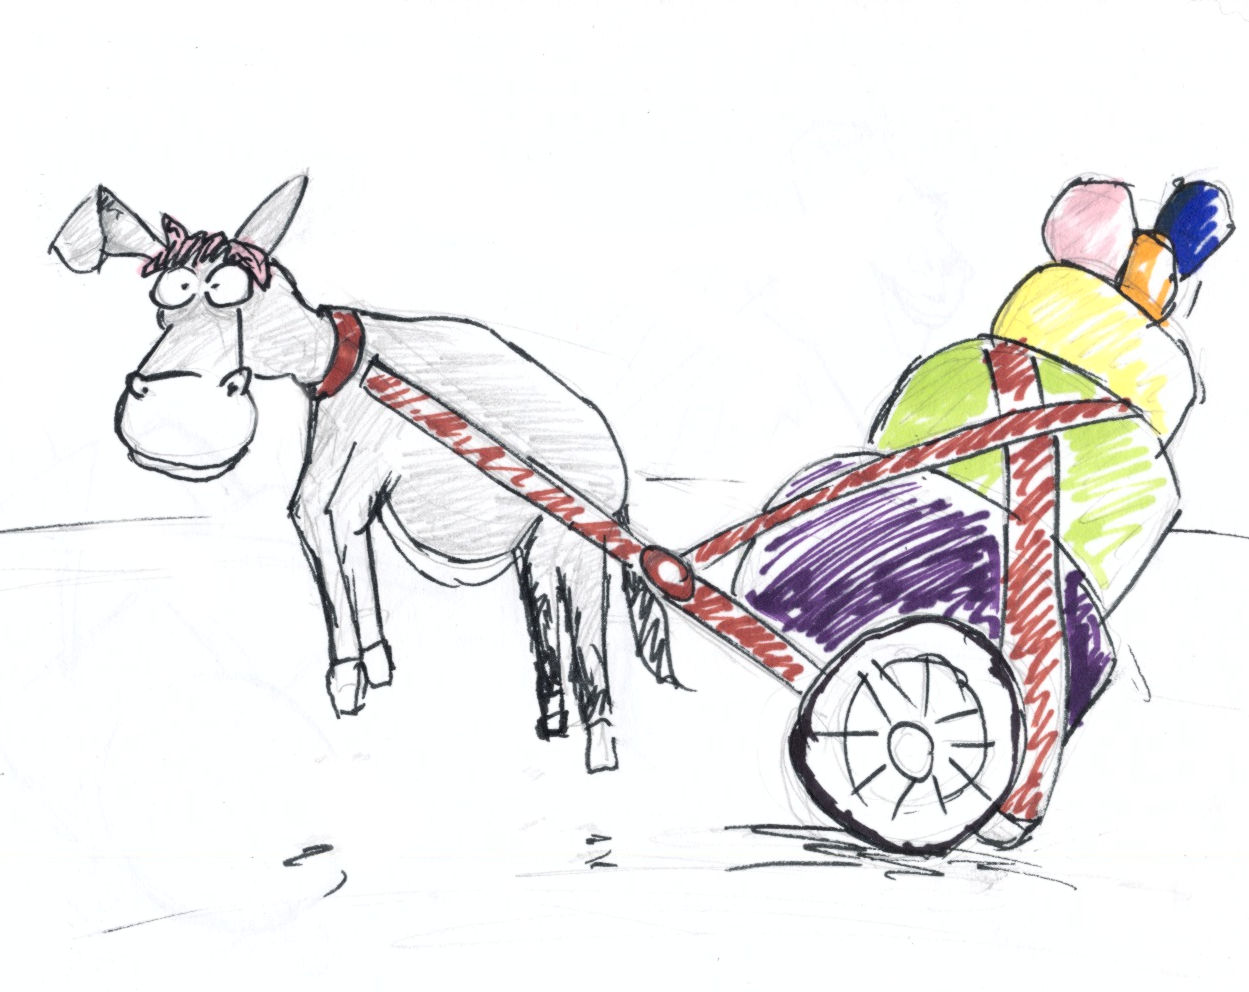
\includegraphics{./images/overload.jpg}

}

\caption{While the frontend is busy looking spiffy, the backend does the
computation work. (Source: own illustration.)}

\end{figure}

Under-the-hood-work that is traditionally implemented in languages like
Java, Python\index{Python} or\index{PHP} PHP\footnote{Yes, one could
  lists JavaScript\index{JavaScript} here, too, but let's keep things
  simple and think of JavaScript\index{JavaScript} as traditionally
  client-side here.} can now be done in R. This is not only convenient
for the R developer who does not need to learn Java, it's also
incredibly comfy if you got data work to do. Or put differently: who
would like to implement logistic regression, random forests or principal
component analysis in PHP?

Consider the following minimal backend \emph{server.R} file which
corresponds to the above \emph{ui.R} frontend file. The anonymous
(nameless) function which is passed on to the \emph{ShinyServer}
function takes two named lists, \emph{input} and \emph{output}, as
arguments. The named elements of the input list correspond to the
\emph{widgetId} parameter of the UI element. In the below example, our
well-known base R function \emph{rnorm} takes \emph{nobs} from the input
as its \emph{n} sample size argument. Mean and standard deviation are
set in the same fashion using the user interface (UI) inputs.

\begin{Shaded}
\begin{Highlighting}[]
\FunctionTok{library}\NormalTok{(shiny)}

\FunctionTok{shinyServer}\NormalTok{(}\ControlFlowTok{function}\NormalTok{(input,output)\{}
  
\NormalTok{  output}\SpecialCharTok{$}\NormalTok{dist }\OtherTok{\textless{}{-}} \FunctionTok{renderPlot}\NormalTok{(\{}
    \FunctionTok{hist}\NormalTok{(}
      \FunctionTok{rnorm}\NormalTok{(input}\SpecialCharTok{$}\NormalTok{nobs,}
            \AttributeTok{mean =}\NormalTok{ input}\SpecialCharTok{$}\NormalTok{mean\_in,}
            \AttributeTok{sd =}\NormalTok{ input}\SpecialCharTok{$}\NormalTok{sd\_in),}
      \AttributeTok{main =} \StringTok{""}\NormalTok{,}
      \AttributeTok{xlab =} \StringTok{""}
\NormalTok{      )}
\NormalTok{  \})}
  
\NormalTok{  output}\SpecialCharTok{$}\NormalTok{tab }\OtherTok{\textless{}{-}} \FunctionTok{renderDataTable}\NormalTok{(\{}
\NormalTok{    mtcars}
\NormalTok{  \})  }
\NormalTok{\})}
\end{Highlighting}
\end{Shaded}

The vector that is returned from \emph{rnorm} is passed on to the base R
\emph{hist} which returns a histogram plot. This plot is then rendered
and stored into an element of the \emph{output} list. The \emph{dist}
name is arbitrary, but again it matched to the UI. The \emph{plotOutput}
function of \emph{ui.R} puts the rendered plot onto the canvas, so it's
on display in people's browsers. \emph{renderDataTable} does so in
analog fashion to render and display the data table.

\hypertarget{put-things-together-and-run-your-app}{%
\subsection{Put Things Together and Run Your
App}\label{put-things-together-and-run-your-app}}

The basic app shown above consists of an \emph{ui.R} and a
\emph{server.R} file living in the same folder. The most straightforward
way to run such an app is to call the \emph{runApp()} function and
provide the location of the folder that contains both of the
aforementioned files.

\begin{Shaded}
\begin{Highlighting}[]
\FunctionTok{library}\NormalTok{(shiny)}
\FunctionTok{runApp}\NormalTok{(}\StringTok{"folder/that/holds/ui\_n\_server"}\NormalTok{)}
\end{Highlighting}
\end{Shaded}

This will use your machine's built-in web server and run
Shiny\index{Shiny} locally on your notebook or desktop computer. Even if
you never put your app on a web server and run a website with it, it is
already a legitimate way to distribute your app. If it was part of an R
package, everyone who downloads your package could use it locally, maybe
as a visual inspection tool or a way to derive inputs interactively and
feed them into your R calculation.

\hypertarget{serve-your-app}{%
\subsection{Serve Your App}\label{serve-your-app}}

Truth be told, the full hype and excitement of a Shiny\index{Shiny} app
only comes into play when you publish your app and make it available to
anyone with a browser, not just the R people. Though hosting is a
challenge in itself, let me provide you a quick Shiny specific
discussion here. The most popular options to host a Shiny app are

\begin{itemize}
\item
  \textbf{Software-as-a-service (SaaS)}\index{SaaS}. No maintenance,
  hassle-free, but least bang for the buck. The fastest way to hit the
  ground running is R Studio's service \emph{shinyapps.io}.
\item
  \textbf{On premise, aka in-house}. Either download the open source
  version of Shiny server, the alternative Shiny proxy or the Posit
  Connect premium solution and install them on your own Virtual Machine.
\item
  Use a \textbf{Shiny server Docker image}\index{Docker} and run a
  container in your preferred environment.
\end{itemize}

\hypertarget{shiny-resources}{%
\subsection{\texorpdfstring{Shiny
Resources\index{Shiny}}{Shiny Resources}}\label{shiny-resources}}

One of the cool things of learning shiny is how Shiny, and its
ecosystem, allow you to learn quickly. Here are some of my favorite
resources to hone your Shiny skills.

\begin{figure}

{\centering 
\includegraphics{./images/blank_dashboard.png}

}

\caption{The \{shinydashboard\} R package provides nice, customizable
skeletons for dashboards. (Source: screenshot of minimal, blank
dashboard created with shinydashboard.)}

\end{figure}

\begin{itemize}
\item
  R Studio Shiny's Widget Gallery:
  https://shiny.rstudio.com/gallery/widget-gallery.html
\item
  shinydashboard (Chang and Borges Ribeiro 2021):
  https://rstudio.github.io/shinydashboard
\item
  Mastering Shiny (Hadley Wickham 2021): (https://mastering-shiny.org/)
\item
  Engineering Production Grade Shiny Apps (Fay et al. 2021):
  https://engineering-shiny.org/
\item
  RInterface by David Granjon, John Coene, Victor Perrier and Isabelle
  Rudolf: https://rinterface.com/
\end{itemize}

\hypertarget{project-management-basics}{%
\section{\texorpdfstring{Project Management
Basics\index{Project Management}}{Project Management Basics}}\label{project-management-basics}}

The art of stress-free productivity, as I once called it in 2010 blog
post, has put a number of gurus on the map and a whole strand of
literature on our bookshelves. So, rather than adding to that, I would
like to extract a healthy, best-of-breed type of dose here. The
following few paragraphs do not intend to be comprehensive, not even for
the scope of software projects, but inspirational.

In the software development startup community, the \emph{waterfall}
approach became synonymous to conservative, traditional and ancient:
Over specification in advance of the project, premature optimization and
a lawsuit over expectations that weren't met. Though, waterfall projects
may be better than their reputation, specifications should not be too
detailed and rigid.

Many software projects are rather organized in \emph{agile} fashion,
with SCRUM\index{SCRUM} and KANBAN being the most popular derivatives.
Because empirical academic projects have a lot in common with software
projects inasmuch that there is a certain expectation and quality
control, but the outcome is not known in advance. Essentially, in agile
project management you roughly define an outcome similar to a minimum
viable product (MVP). That way, you do not end up with nothing after a
year of back and forth. During the implementation you'd meet regularly,
let's say every 10 days, to discuss development since the last meet and
the short-term plans for the steps ahead. The team splits work into
tasks on the issue tracker and assigns them. Solutions to problems will
only be sketched out and discussed bilaterally or in small groups. By
defining the work package for only a short timespan, the team stays
flexible. In professional setups, agile development is often strictly
implemented and makes use of sophisticated systems of roles that
developers and project managers can get certified for.

Major git platforms ship with a decent, carpentry-level project
management\index{Project Management} GUI. The issue tracker is at the
core of this. If you use it the minimal way, it's simply a colorful
to-do list. Yet, with a bit of inspiration and the use of tags, comments
and projects, an issue tracker can be a lot more.

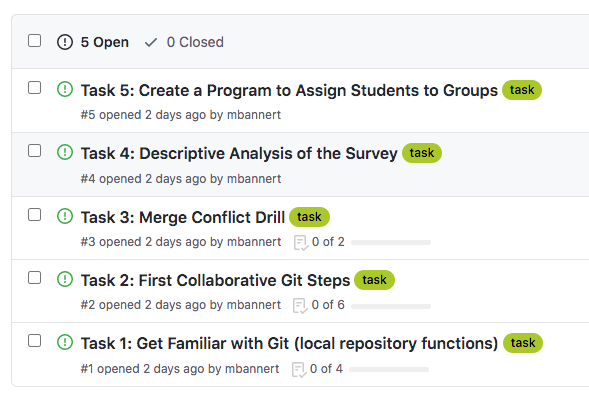
\includegraphics{./images/issue.png}

The GitHub\index{GitHub} issue tracker (example from one of the course's
repositories) can be a lot more than a to-do list.

Swim lanes (reminiscent of a bird's-eye view of an Olympic pool) can be
thought of columns that you have to walk through from left to right: To
Do, Doing, Under Review, done. (you can also customize the number and
label of lanes and event associate actions with them, but let's stick to
those basic lanes in this section.) The idea is to use to keep track of
the process and make the process transparent.

\begin{figure}

{\centering 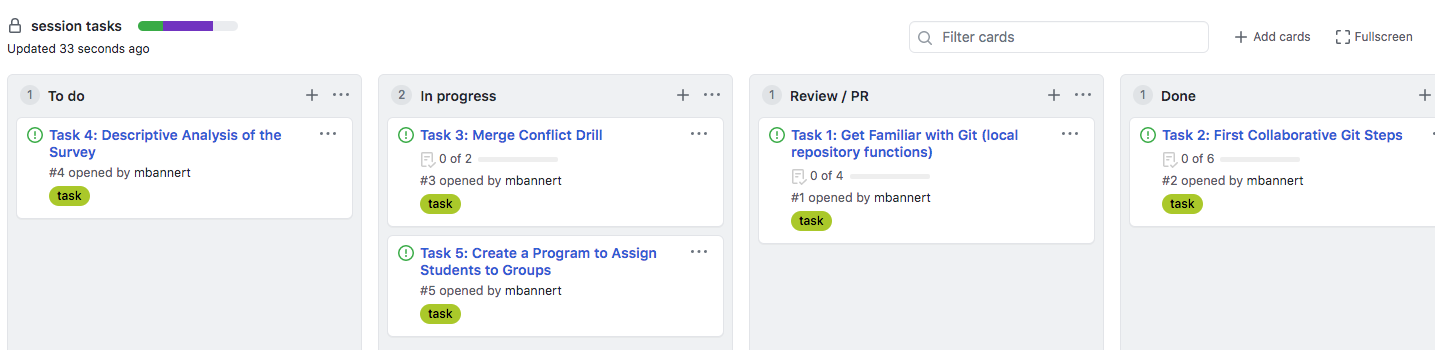
\includegraphics{./images/swim.png}

}

\caption{GitHub's web platform offers swim lanes to keep a better
overview of issues being worked on. (Source: own GitHub repository.)}

\end{figure}

\begin{tcolorbox}[enhanced jigsaw, left=2mm, arc=.35mm, colbacktitle=quarto-callout-tip-color!10!white, breakable, colframe=quarto-callout-tip-color-frame, bottomrule=.15mm, bottomtitle=1mm, colback=white, leftrule=.75mm, coltitle=black, toptitle=1mm, titlerule=0mm, title=\textcolor{quarto-callout-tip-color}{\faLightbulb}\hspace{0.5em}{Tip}, opacityback=0, rightrule=.15mm, toprule=.15mm, opacitybacktitle=0.6]

No lane except ``Done'' should contain more than 5--6 issues. Doing so
prevents clogging the lanes at a particular stage which could
potentially lead to negligent behavior, e.g., careless reviews.

\end{tcolorbox}

\hypertarget{parallel-computation}{%
\section{Parallel Computation}\label{parallel-computation}}

The idea of having multiple workers at your disposal to fix your math
problem even quicker than one smart worker seems equally appealing to
third graders and researchers. Very much like in school, the ability to
assess whether getting help in the first place is worth the overhead and
what type of help to get, is the most important skill. The classical
challenge where parallel computation using multiple cores really helps
is throughput problems, i.e., problems where your tasks are independent
of each other. Yet, it may not be clear up-front if the number and
computation time of your single tasks justifies the overhead of letting
your program know it should split computations across cores and manage
memory accordingly. Also, consider that processes can be turned parallel
at different levels: you could simply use your local machine's cores and
a parallelization implementation such as R's \{future\} (Bengtsson 2021)
or \{parallel\} packages to parrallelize locally. Or you could go
parallel at a machine or container level. While the former is easier as
it requires less infrastructure\index{infrastructure} knowledge, it is
limited by the resources of your local machine. Of course, if you have
access to a HPC cluster, this may not be a disadvantage at all
(depending on how your cluster balances load and manages access to
resources). In any case, you should make a clear decision at which level
you go parallel and avoid nested parallelization.

Let's consider the following example of a simple local parallelization,
including a performance benchmark. The following R example uses the
\{microbenchmark\} R package (Mersmann 2021) to check the effect of
parallel computing on running seasonal adjustment of multiple time
series\index{time series}. Before we start with the actual example,
let's create some demo data: We simply create a list with 1000 elements,
each of which is the same monthly time series\index{time series} about
airline passengers from 1949 to 1960.

\begin{Shaded}
\begin{Highlighting}[]
\FunctionTok{data}\NormalTok{(}\StringTok{"AirPassengers"}\NormalTok{)}
\NormalTok{tsl }\OtherTok{\textless{}{-}} \FunctionTok{list}\NormalTok{()}
\ControlFlowTok{for}\NormalTok{(i }\ControlFlowTok{in} \DecValTok{1}\SpecialCharTok{:}\DecValTok{1000}\NormalTok{)\{}
\NormalTok{  tsl[[i]] }\OtherTok{\textless{}{-}}\NormalTok{ AirPassengers}
\NormalTok{\}}
\end{Highlighting}
\end{Shaded}

Now, let's load the \{seasonal\} R package (Sax and Eddelbuettel 2018)
and perform a basic seasonal adjustment of each of these time
series\index{time series}. The first statement performs 100 adjustments
sequentially; the second statement uses parallel computing to spread
computations across the processors of the machine that ran this example.

\begin{Shaded}
\begin{Highlighting}[]
\FunctionTok{library}\NormalTok{(seasonal)}
\FunctionTok{library}\NormalTok{(parallel)}
\FunctionTok{library}\NormalTok{(microbenchmark)}


\NormalTok{no\_parallel }\OtherTok{\textless{}{-}} \ControlFlowTok{function}\NormalTok{(li, s)\{}
  \FunctionTok{lapply}\NormalTok{(li[s],seas)}
\NormalTok{\}}

\NormalTok{with\_parallel }\OtherTok{\textless{}{-}} \ControlFlowTok{function}\NormalTok{(li, s)\{}
\NormalTok{  out }\OtherTok{\textless{}{-}} \FunctionTok{list}\NormalTok{()}
\NormalTok{  cl }\OtherTok{\textless{}{-}} \FunctionTok{makeCluster}\NormalTok{(}\FunctionTok{detectCores}\NormalTok{())}
  \CommentTok{\# load \textquotesingle{}seasonal\textquotesingle{} for each node}
  \FunctionTok{clusterEvalQ}\NormalTok{(cl, }\FunctionTok{library}\NormalTok{(seasonal))}
  \FunctionTok{parLapply}\NormalTok{(cl, li[s], }\ControlFlowTok{function}\NormalTok{(e) }\FunctionTok{try}\NormalTok{(}\FunctionTok{seas}\NormalTok{(e)))}
  \FunctionTok{stopCluster}\NormalTok{(cl)}
\NormalTok{\}}


\NormalTok{out }\OtherTok{\textless{}{-}} \FunctionTok{microbenchmark}\NormalTok{(}
    \AttributeTok{noparallel10 =} \FunctionTok{no\_parallel}\NormalTok{(tsl, }\DecValTok{1}\SpecialCharTok{:}\DecValTok{10}\NormalTok{),}
    \AttributeTok{withparallel10 =} \FunctionTok{with\_parallel}\NormalTok{(tsl, }\DecValTok{1}\SpecialCharTok{:}\DecValTok{10}\NormalTok{),}
    \AttributeTok{noparallel100 =} \FunctionTok{no\_parallel}\NormalTok{(tsl, }\DecValTok{1}\SpecialCharTok{:}\DecValTok{100}\NormalTok{),}
    \AttributeTok{withparallel100 =} \FunctionTok{with\_parallel}\NormalTok{(tsl, }\DecValTok{1}\SpecialCharTok{:}\DecValTok{100}\NormalTok{),}
    \AttributeTok{times =} \DecValTok{5}\NormalTok{,}
    \AttributeTok{unit =} \StringTok{"seconds"}
\NormalTok{)}

\NormalTok{d }\OtherTok{\textless{}{-}} \FunctionTok{summary}\NormalTok{(out)}
\end{Highlighting}
\end{Shaded}

Obviously, the absolute computation time depends on the hardware used as
well as the operating system, depending on the task at hand.

As expected, given the perfect independence of the tasks from each
other, performance gains are quite substantial (\textasciitilde5.5 times
faster) for the above example, though not perfect (on my 8-core
machine). Advanced parallel implementations and deeper dives into the
way different processors work may further optimize efficiency here.

\begin{Shaded}
\begin{Highlighting}[]
\FunctionTok{library}\NormalTok{(kableExtra)}
\FunctionTok{kable}\NormalTok{(d[,}\FunctionTok{c}\NormalTok{(}\DecValTok{1}\SpecialCharTok{:}\DecValTok{4}\NormalTok{)],}\StringTok{"latex"}\NormalTok{,}
      \AttributeTok{booktabs =} \ConstantTok{TRUE}\NormalTok{,}
      \AttributeTok{escape=} \ConstantTok{FALSE}\NormalTok{) }\SpecialCharTok{|\textgreater{}}
      \FunctionTok{kable\_styling}\NormalTok{(}
        \AttributeTok{latex\_options =} \FunctionTok{c}\NormalTok{(}\StringTok{"repeat\_header"}\NormalTok{)}
\NormalTok{        ) }\SpecialCharTok{|\textgreater{}}
      \FunctionTok{column\_spec}\NormalTok{(}\DecValTok{1}\SpecialCharTok{:}\DecValTok{2}\NormalTok{, }\AttributeTok{width =} \StringTok{"2.5cm"}\NormalTok{)}
\FunctionTok{kable}\NormalTok{(d[,}\FunctionTok{c}\NormalTok{(}\DecValTok{1}\NormalTok{,}\DecValTok{5}\NormalTok{,}\DecValTok{6}\NormalTok{,}\DecValTok{7}\NormalTok{)],}\StringTok{"latex"}\NormalTok{,}
      \AttributeTok{booktabs =} \ConstantTok{TRUE}\NormalTok{,}
      \AttributeTok{escape=} \ConstantTok{FALSE}\NormalTok{) }\SpecialCharTok{|\textgreater{}}
      \FunctionTok{kable\_styling}\NormalTok{(}
        \AttributeTok{latex\_options =} \FunctionTok{c}\NormalTok{(}\StringTok{"repeat\_header"}\NormalTok{)}
\NormalTok{        ) }\SpecialCharTok{|\textgreater{}}
      \FunctionTok{column\_spec}\NormalTok{(}\DecValTok{1}\SpecialCharTok{:}\DecValTok{2}\NormalTok{, }\AttributeTok{width =} \StringTok{"2.5cm"}\NormalTok{)}
\end{Highlighting}
\end{Shaded}

\begin{table}

\caption{\label{tbl-benchmark}Runtimes with and without
parallelization.}\begin{minipage}[t]{\linewidth}
\subcaption{\label{tbl-benchmark-1}}

{\centering 

\centering
\begin{tabular}{>{\raggedright\arraybackslash}p{2.5cm}>{\raggedleft\arraybackslash}p{2.5cm}rr}
\toprule
expr & min & lq & mean\\
\midrule
noparallel10 & 1.9800640 & 1.984759 & 1.9974641\\
withparallel10 & 0.6584706 & 0.670383 & 0.6801107\\
noparallel100 & 20.0615293 & 20.093228 & 20.2760411\\
withparallel100 & 3.5213346 & 3.560120 & 3.6941739\\
\bottomrule
\end{tabular}

}

\end{minipage}%
\newline
\begin{minipage}[t]{\linewidth}
\subcaption{\label{tbl-benchmark-2}}

{\centering 

\centering
\begin{tabular}{>{\raggedright\arraybackslash}p{2.5cm}>{\raggedleft\arraybackslash}p{2.5cm}rr}
\toprule
expr & median & uq & max\\
\midrule
noparallel10 & 1.9995083 & 2.0057684 & 2.0172208\\
withparallel10 & 0.6773499 & 0.6882694 & 0.7060808\\
noparallel100 & 20.1384522 & 20.3897492 & 20.6972465\\
withparallel100 & 3.6266411 & 3.8025281 & 3.9602453\\
\bottomrule
\end{tabular}

}

\end{minipage}%

\end{table}

Yet, the key takeaway from the above exercise is not the parallel
computation itself, but the ability to evaluate the need to go parallel
and how. Benchmarking does not only help to get a ballpark estimate of
the costs should you go outside for more computational power, it gives
you an idea whether the gains from a parallel approach are worth the
hassle. In other words, of course a computation running four to five
times faster than before sounds spectacular, but what if the total
runtime is less than a few minutes either way? Development time,
particularly for newcomers, is very likely longer than a few minutes.
Plus, going parallel jeopardizes your cross-platform compatibility
depending on the parallel implementation you use.

Another good use of benchmarking is to run a few smaller case
experiments to get an idea of how performance gains evolves when we
throw more work at our system. Unlike the below example, performance
gains do not necessarily have to be linear. Visualization can give us a
better idea.

\begin{Shaded}
\begin{Highlighting}[]
\FunctionTok{library}\NormalTok{(ggplot2)}
\FunctionTok{library}\NormalTok{(viridis)}
\NormalTok{vizframe }\OtherTok{\textless{}{-}}\NormalTok{ d[,}\FunctionTok{c}\NormalTok{(}\DecValTok{1}\NormalTok{,}\DecValTok{5}\NormalTok{)]}
\NormalTok{vizframe}\SpecialCharTok{$}\NormalTok{iterations }\OtherTok{\textless{}{-}} \FunctionTok{as.character}\NormalTok{(}\FunctionTok{c}\NormalTok{(}\DecValTok{10}\NormalTok{,}\DecValTok{10}\NormalTok{,}\DecValTok{100}\NormalTok{,}\DecValTok{100}\NormalTok{))}
\NormalTok{vizframe}\SpecialCharTok{$}\NormalTok{parallel }\OtherTok{\textless{}{-}} \FunctionTok{c}\NormalTok{(}\StringTok{"no"}\NormalTok{,}\StringTok{"yes"}\NormalTok{,}\StringTok{"no"}\NormalTok{,}\StringTok{"yes"}\NormalTok{)}
\FunctionTok{names}\NormalTok{(vizframe)[}\DecValTok{2}\NormalTok{] }\OtherTok{\textless{}{-}} \StringTok{"seconds"}

\NormalTok{gg }\OtherTok{\textless{}{-}} \FunctionTok{ggplot}\NormalTok{(}
\NormalTok{  vizframe[,}\SpecialCharTok{{-}}\DecValTok{1}\NormalTok{],}
 \FunctionTok{aes}\NormalTok{(}\AttributeTok{fill =}\NormalTok{ parallel, }
     \AttributeTok{y =}\NormalTok{ seconds,}
     \AttributeTok{x =}\NormalTok{ iterations))}
\NormalTok{gg }\SpecialCharTok{+} 
  \FunctionTok{geom\_bar}\NormalTok{(}\AttributeTok{position =} \StringTok{"dodge"}\NormalTok{,}
           \AttributeTok{stat =} \StringTok{"identity"}\NormalTok{) }\SpecialCharTok{+} 
  \FunctionTok{coord\_flip}\NormalTok{() }\SpecialCharTok{+} 
  \FunctionTok{scale\_fill\_viridis}\NormalTok{(}\AttributeTok{discrete =}\NormalTok{ T) }\SpecialCharTok{+}
  \FunctionTok{theme\_minimal}\NormalTok{()}
\end{Highlighting}
\end{Shaded}

\begin{figure}[H]

{\centering 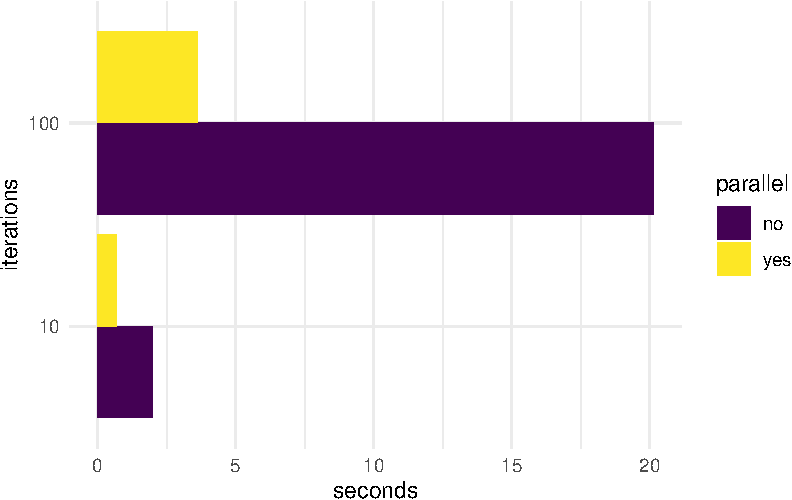
\includegraphics{./case-studies_files/figure-pdf/fig-benchmark-1.pdf}

}

\caption{\label{fig-benchmark}Comparison of computation time (shorter
bar is faster).}

\end{figure}

\hypertarget{good-practice}{%
\section{\texorpdfstring{Good
Practice\index{Good Practice}}{Good Practice}}\label{good-practice}}

Even though I cannot really aim for a comprehensive section on the
\emph{Do's and Dont's}, I would like to share a few common-sense
practices here. If you are interested in a more thorough but rather R
specific collection, take a look at the wonderful online book \emph{What
They Forgot to Tell Us About R}: https://rstats.wtf/.

\textbf{Do NOT Set Static Working Directories in Your Code}

Like
\texttt{C:\textbackslash{}Users\textbackslash{}MatthiasBannert\textbackslash{}My\ Documents\textbackslash{}R\ Course\textbackslash{}}.
Locations that only exist in your own environment have you set up for
trouble before you even started.

Please,

\begin{itemize}
\item
  resist that visceral urge to define the project root folder somewhere
  at the beginning of your code because your collaborators usually do
  not have a directory on their machine that bears your name. That might
  not even use the same operating system. And before you ask, simply
  putting the neutrally named folder on a shared NAS storage or service
  such as Dropbox is not really better.
\item
  avoid spaces in folder and file names. Though modern operating systems
  and most languages can handle spaces, you might need to escape certain
  characters and make a beginner's life much harder. The same holds for
  umlauts and other hieroglyphic characters. Simply use lower-case and
  either kebab-case or snake\_case.
\item
  work with projects of your favorite IDE. The idea of projects is to
  make a folder the document root of your project. That way, your code
  can reference to other files inside this project root in relative
  fashion, no matter where the project itself is located.
\end{itemize}

\textbf{Take Time To Learn How To Play the ``Piano''}

There is no need to become a \emph{vim} virtuoso (that's essentially
Lang Lang status on a computer keyboard), but make sure to learn some
basic shortcuts of your environment that help you avoid touching the
mouse or trackpad. Like \texttt{ctrl+L} to clear the screen,
\texttt{cmd+tab} to switch between applications, \texttt{cmd+w} to close
windows, \texttt{ctrl+number} to switch between tabs and, most
importantly, some shortcut to execute the selected line of code (often
\texttt{cmd+enter}, \texttt{ctrl+enter} or \texttt{shift+enter}
depending on your operating system). Note that this is really not so
much about a specific programming language, but more about the
environment you work in.

\textbf{Manage Dependencies at the Project Level}

JavaScript\index{JavaScript} projects manage dependencies in their lock
files, Python projects have their requirements.txt files, and R has the
\{renv\} package (Ushey and Wickham 2023). All these scripting languages
\emph{can} keep track of the exact library versions used in a project.

\begin{Shaded}
\begin{Highlighting}[]
\ExtensionTok{pip}\NormalTok{ freeze }\KeywordTok{|}
 \FunctionTok{grep} \AttributeTok{{-}v} \StringTok{"pkg{-}resources"} \OperatorTok{\textgreater{}}\NormalTok{ requirements.txt}
\end{Highlighting}
\end{Shaded}

The above pip command extracts dependencies from a Python project's
folder and writes it to a requirements file. Nevertheless, because there
is no build process, scripting languages do not enforce keeping track of
library versions necessarily. And even though it is common sense in
engineering, it took data science, R in particular, quite a while to
really establish going the extra mile and keep track of a project's
dependencies. For many, an R \emph{project A} simply loads a few
libraries, does its job, while another \emph{R project B} loads its
libraries and does another job -- all on the same local machine. After a
few more projects, we decided to upgrade R to the next minor release,
e.g., go from 4.1. to 4.2. which cause reinstalling all the extensions
packages. It is a very safe bet that at least one of the packages we use
gets its own update (or two) between two R minor releases. When all
projects share the same library, your project that has just started
after the latest package release may benefit from the latest feature of
a package, while another project might break because its code is
affected by a breaking change. Given that most packages are not large in
size, I encourage everyone starting a programming with data project to
embrace project-based library version management early on.

\bookmarksetup{startatroot}

\hypertarget{glossary}{%
\chapter*{Glossary}\label{glossary}}

\markboth{Glossary}{Glossary}

\begin{longtable}{l>{\raggedright\arraybackslash}p{6.8cm}}
\toprule
Term & Description\\
\midrule
\endfirsthead
\multicolumn{2}{@{}l}{\textit{(continued)}}\\
\toprule
Term & Description\\
\midrule
\endhead

\endfoot
\bottomrule
\endlastfoot
API & Application Programming Interface\\
CamelCase & Convention to spell file, variable or function names reminiscent of a camel, e.g., doSomething().\\
CMS & Content Management System.\\
Console & Also known as terminal, the console is an interface which takes written user commands. Bash is one of the most popular terminals on OS level, but scripting languages like Python and R have consoles to communicate with their interpreter,too.\\
Deployment & The art of delivering a piece of software to production.\\
\addlinespace
Endpoint & Part of an API, a generic URL that follows a logic that can be exploited to automate machine-to-machine data exchange.\\
Fork & A clone of a repository that you (usually) do not own.\\
GUI & Graphical User Interface.\\
IDE & Integrated Development Environment.\\
Kebab Case & Spelling convention less known than snake case and camel case, kebap case looks like this: my-super-folder.\\
\addlinespace
Lexical Scoping & Look-up of variables in parent environments when they can't be found in the current environment. Be aware that this is the default behavior of R.\\
Merge Request & See Pull Request.\\
OS & Operating System.\\
OSS & Open Source Software.\\
Pull Request (PR) & Request to join a feature branch into another branch, e.g., main branch. Sometimes it's also called merge request.\\
\addlinespace
Regular Expression & Pattern to extract specific parts from a text, find stuff in a text.\\
REPL & read-eval-print-loop.\\
Reproducible Example & A self-contained code example, including the data it needs to run.\\
Reverse Dependency & Inverted dependency, another library or piece of code that depends on the code at hand.\\
Snake\_case & Convention to spell file, variable or function names reminiscant of a snake, e.g., do\_something().\\
\addlinespace
Stack & selection of software used in a project.\\
SQL & Structured Query Language.\\
Swimlanes & (Online) Board of columns (lanes). Lanes progress from from left to right and carry issues.\\
Throughput Problem & A bottleneck which can be mitigated by parallelization, e.g., multiple containers running in parallel.\\
Transactional database & database optimized for production systems. Such a database is good at reading and writing individual rows without affecting the other and while taking care of data integrity.\\
\addlinespace
Virtual Machine (VM) & A virtual computer hosted on your computer. Often used to run another OS inside your main OS for testing purposes.\\*
\end{longtable}

\bookmarksetup{startatroot}

\hypertarget{references}{%
\chapter*{References}\label{references}}

\markboth{References}{References}

\hypertarget{refs}{}
\begin{CSLReferences}{1}{0}
\leavevmode\vadjust pre{\hypertarget{ref-Quarto}{}}%
Allaire, J. J., Charles Teague, Carlos Scheidegger, Yihui Xie, and
Christophe Dervieux. 2022. \emph{{Quarto}} (version 1.2).
\url{https://doi.org/10.5281/zenodo.5960048}.

\leavevmode\vadjust pre{\hypertarget{ref-rmarkdown}{}}%
Allaire, JJ, Yihui Xie, Jonathan McPherson, Javier Luraschi, Kevin
Ushey, Aron Atkins, Hadley Wickham, Joe Cheng, Winston Chang, and
Richard Iannone. 2022. \emph{Rmarkdown: Dynamic Documents for r}.
\url{https://github.com/rstudio/rmarkdown}.

\leavevmode\vadjust pre{\hypertarget{ref-kofdata}{}}%
Bannert, Matthias, and Severin Thoeni. 2022. \emph{Kofdata: Get Data
from the 'KOF Datenservice' API}.
\url{https://CRAN.R-project.org/package=kofdata}.

\leavevmode\vadjust pre{\hypertarget{ref-tstools}{}}%
Bannert, Matthias, Severin Thoeni, and Stéphane Bisinger. 2023.
\emph{Tstools: A Time Series Toolbox for Official Statistics}.
\url{https://CRAN.R-project.org/package=tstools}.

\leavevmode\vadjust pre{\hypertarget{ref-jupyter}{}}%
Beg, Marijan, Juliette Taka, Thomas Kluyver, Olexandr Konovalov, Min
Ragan-Kelly, Nicolas M. Thiéry, and Hans Fangohr. 2021. {``Using Jupyter
for Reproducible Scientific Workflows.''} \emph{CoRR} abs/2102.09562.
\url{https://arxiv.org/abs/2102.09562}.

\leavevmode\vadjust pre{\hypertarget{ref-future}{}}%
Bengtsson, Henrik. 2021. {``A Unifying Framework for Parallel and
Distributed Processing in r Using Futures.''} \emph{The R Journal} 13
(2): 208--27. \url{https://doi.org/10.32614/RJ-2021-048}.

\leavevmode\vadjust pre{\hypertarget{ref-julia}{}}%
Bezanson, Jeff, Alan Edelman, Stefan Karpinski, and Viral B Shah. 2017.
{``Julia: A Fresh Approach to Numerical Computing.''} \emph{SIAM Review}
59 (1): 65--98. \url{https://doi.org/10.1137/141000671}.

\leavevmode\vadjust pre{\hypertarget{ref-d3}{}}%
Bostock, Michael, Vadim Ogievetsky, and Jeffrey Heer. 2011. {``D³
Data-Driven Documents.''} \emph{IEEE Transactions on Visualization and
Computer Graphics} 17 (12): 2301--9.
\url{https://doi.org/10.1109/TVCG.2011.185}.

\leavevmode\vadjust pre{\hypertarget{ref-r6}{}}%
Chang, Winston. 2021. \emph{R6: Encapsulated Classes with Reference
Semantics}. \url{https://CRAN.R-project.org/package=R6}.

\leavevmode\vadjust pre{\hypertarget{ref-shinydashboard}{}}%
Chang, Winston, and Barbara Borges Ribeiro. 2021. \emph{Shinydashboard:
Create Dashboards with 'Shiny'}.
\url{https://CRAN.R-project.org/package=shinydashboard}.

\leavevmode\vadjust pre{\hypertarget{ref-shiny}{}}%
Chang, Winston, Joe Cheng, JJ Allaire, Carson Sievert, Barret Schloerke,
Yihui Xie, Jeff Allen, Jonathan McPherson, Alan Dipert, and Barbara
Borges. 2022. \emph{Shiny: Web Application Framework for r}.
\url{https://CRAN.R-project.org/package=shiny}.

\leavevmode\vadjust pre{\hypertarget{ref-distill}{}}%
Dervieux, Christophe, JJ Allaire, Rich Iannone, Alison Presmanes Hill,
and Yihui Xie. 2022. \emph{Distill: 'R Markdown' Format for Scientific
and Technical Writing}.
\url{https://CRAN.R-project.org/package=distill}.

\leavevmode\vadjust pre{\hypertarget{ref-fay2021engineering}{}}%
Fay, C., S. Rochette, V. Guyader, and C. Girard. 2021. \emph{Engineering
Production-Grade Shiny Apps}. Chapman \& Hall/CRC the r Series. CRC
Press. \url{https://books.google.ch/books?id=qExDEAAAQBAJ}.

\leavevmode\vadjust pre{\hypertarget{ref-cffr}{}}%
Hernangómez, Diego. 2021. {``Cffr: Generate Citation File Format
Metadata for r Packages.''} \emph{Journal of Open Source Software} 6
(67): 3900. \url{https://doi.org/10.21105/joss.03900}.

\leavevmode\vadjust pre{\hypertarget{ref-matplotlib}{}}%
Hunter, J. D. 2007. {``Matplotlib: A 2D Graphics Environment.''}
\emph{Computing In Science \& Engineering} 9 (3): 90--95.

\leavevmode\vadjust pre{\hypertarget{ref-inclusivecon}{}}%
Joo, Rocío et al. 2022. {``Ten Simple Rules to Host an Inclusive
Conference.''} \emph{PLOS Computational Biology} 18 (7): 1--13.
\url{https://doi.org/10.1371/journal.pcbi.1010164}.

\leavevmode\vadjust pre{\hypertarget{ref-targets}{}}%
Landau, William Michael. 2021. {``The Targets r Package: A Dynamic
Make-Like Function-Oriented Pipeline Toolkit for Reproducibility and
High-Performance Computing.''} \emph{Journal of Open Source Software} 6
(57): 2959. \url{https://doi.org/10.21105/joss.02959}.

\leavevmode\vadjust pre{\hypertarget{ref-echarts}{}}%
Li, Deqing, Honghui Mei, Yi Shen, Shuang Su, Wenli Zhang, Junting Wang,
Ming Zu, and Wei Chen. 2018. {``ECharts: A Declarative Framework for
Rapid Construction of Web-Based Visualization.''} \emph{Visual
Informatics} 2 (2): 136--46.
https://doi.org/\url{https://doi.org/10.1016/j.visinf.2018.04.011}.

\leavevmode\vadjust pre{\hypertarget{ref-microbenchmark}{}}%
Mersmann, Olaf. 2021. \emph{Microbenchmark: Accurate Timing Functions}.
\url{https://CRAN.R-project.org/package=microbenchmark}.

\leavevmode\vadjust pre{\hypertarget{ref-gganimate}{}}%
Pedersen, Thomas Lin, and David Robinson. 2022. \emph{Gganimate: A
Grammar of Animated Graphics}.
\url{https://CRAN.R-project.org/package=gganimate}.

\leavevmode\vadjust pre{\hypertarget{ref-polite}{}}%
Perepolkin, Dmytro. 2023. \emph{Polite: Be Nice on the Web}.
\url{https://CRAN.R-project.org/package=polite}.

\leavevmode\vadjust pre{\hypertarget{ref-arrow}{}}%
Richardson, Neal, Ian Cook, Nic Crane, Dewey Dunnington, Romain
François, Jonathan Keane, Dragoș Moldovan-Grünfeld, Jeroen Ooms, and
Apache Arrow. 2022. \emph{Arrow: Integration to 'Apache' 'Arrow'}.
\url{https://CRAN.R-project.org/package=arrow}.

\leavevmode\vadjust pre{\hypertarget{ref-seasonal}{}}%
Sax, Christoph, and Dirk Eddelbuettel. 2018. {``Seasonal Adjustment by
{X-13ARIMA-SEATS} in {R}.''} \emph{Journal of Statistical Software} 87
(11): 1--17. \url{https://doi.org/10.18637/jss.v087.i11}.

\leavevmode\vadjust pre{\hypertarget{ref-plumbr}{}}%
Schloerke, Barret, and Jeff Allen. 2022. \emph{Plumber: An API Generator
for r}. \url{https://CRAN.R-project.org/package=plumber}.

\leavevmode\vadjust pre{\hypertarget{ref-sink}{}}%
Sink, Eric. 2011. \emph{Version Control by Example}. 1st ed. PYOW Sports
Marketing.

\leavevmode\vadjust pre{\hypertarget{ref-renv}{}}%
Ushey, Kevin, and Hadley Wickham. 2023. \emph{Renv: Project
Environments}. \url{https://CRAN.R-project.org/package=renv}.

\leavevmode\vadjust pre{\hypertarget{ref-tinytest}{}}%
van der Loo, MPJ. 2020. {``A Method for Deriving Information from
Running r Code.''} \emph{The R Journal}, Accepted for publication.
\url{https://arxiv.org/abs/2002.07472}.

\leavevmode\vadjust pre{\hypertarget{ref-soscieds}{}}%
Vilhuber, Lars, Marie Connolly, Miklós Koren, Joan Llull, and Peter
Morrow. 2022. \emph{{A template README for social science replication
packages}}. \url{https://doi.org/10.5281/zenodo.7293838}.

\leavevmode\vadjust pre{\hypertarget{ref-rpkgs}{}}%
Wickham, H. 2015. \emph{R Packages: Organize, Test, Document, and Share
Your Code}. O'Reilly Media. \url{https://r-pkgs.org/}.

\leavevmode\vadjust pre{\hypertarget{ref-testthat}{}}%
Wickham, Hadley. 2011. {``Testthat: Get Started with Testing.''}
\emph{The R Journal} 3: 5--10.
\url{https://journal.r-project.org/archive/2011-1/RJournal_2011-1_Wickham.pdf}.

\leavevmode\vadjust pre{\hypertarget{ref-ggplot}{}}%
---------. 2016. \emph{Ggplot2: Elegant Graphics for Data Analysis}.
Springer-Verlag New York. \url{https://ggplot2.tidyverse.org}.

\leavevmode\vadjust pre{\hypertarget{ref-advancedR}{}}%
---------. 2019. \emph{Advanced r}. 2nd ed. Chapman \& Hall/CRC the r
Series. Taylor \& Francis.

\leavevmode\vadjust pre{\hypertarget{ref-masteringshiny}{}}%
---------. 2021. \emph{Mastering Shiny}. O'Reilly Media, Incorporated.
\url{https://books.google.ch/books?id=ha1CzgEACAAJ}.

\leavevmode\vadjust pre{\hypertarget{ref-rvest}{}}%
---------. 2022a. \emph{Rvest: Easily Harvest (Scrape) Web Pages}.
\url{https://CRAN.R-project.org/package=rvest}.

\leavevmode\vadjust pre{\hypertarget{ref-stringr}{}}%
---------. 2022b. \emph{Stringr: Simple, Consistent Wrappers for Common
String Operations}. \url{https://CRAN.R-project.org/package=stringr}.

\leavevmode\vadjust pre{\hypertarget{ref-usethis}{}}%
Wickham, Hadley, Jennifer Bryan, Malcolm Barrett, and Andy Teucher.
2023. \emph{Usethis: Automate Package and Project Setup}.
\url{https://CRAN.R-project.org/package=usethis}.

\leavevmode\vadjust pre{\hypertarget{ref-roxygen}{}}%
Wickham, Hadley, Peter Danenberg, Gábor Csárdi, and Manuel Eugster.
2022. \emph{Roxygen2: In-Line Documentation for r}.
\url{https://CRAN.R-project.org/package=roxygen2}.

\leavevmode\vadjust pre{\hypertarget{ref-r4ds}{}}%
Wickham, Hadley, and Garrett Grolemund. 2017. \emph{R for Data Science:
Import, Tidy, Transform, Visualize, and Model Data}. 1st ed. O'Reilly
Media, Inc.

\leavevmode\vadjust pre{\hypertarget{ref-pkgdown}{}}%
Wickham, Hadley, Jay Hesselberth, and Maëlle Salmon. 2022.
\emph{Pkgdown: Make Static HTML Documentation for a Package}.
\url{https://CRAN.R-project.org/package=pkgdown}.

\leavevmode\vadjust pre{\hypertarget{ref-blogdown}{}}%
Xie, Yihui, Alison Presmanes Hill, and Amber Thomas. 2017.
\emph{Blogdown: Creating Websites with {R} Markdown}. Boca Raton,
Florida: Chapman; Hall/CRC. \url{https://bookdown.org/yihui/blogdown/}.

\leavevmode\vadjust pre{\hypertarget{ref-soup}{}}%
Zheng, Chunmei, Guomei He, and Zuojie Peng. 2015. {``A Study of Web
Information Extraction Technology Based on Beautiful Soup.''} \emph{J.
Comput.} 10: 381--87.

\end{CSLReferences}



\printindex

\end{document}
